%You can delete all the comments after you have finished your document
%this sets up the defaults for the documents, 12pt font and A4 size. The article type sets this up as such as opposed to letter or memo.

%for the finer points LaTeX see https://en.wikibooks.org/wiki/LaTeX or http://tex.stackexchange.com/

\documentclass[12pt,a4paper]{article}
\usepackage{titlesec} %these are how we import packages, one helps set up footers and title layout
\usepackage{fancyhdr}

% !TEX TS-program = pdflatex
% !TEX encoding = UTF-8 Unicode
\usepackage[utf8]{inputenc} % set input encoding (not needed with XeLaTeX)

\usepackage{graphicx} % support the \includegraphics command and options
\graphicspath{{./images/}}

\usepackage[parfill]{parskip} % Activate to begin paragraphs with an empty line rather than an indent

%%% PACKAGES
\usepackage{booktabs} % for much better looking tables
\usepackage{array} % for better arrays (eg matrices) in maths
\usepackage{paralist} % very flexible & customisable lists (eg. enumerate/itemize, etc.)
\usepackage{verbatim} % adds environment for commenting out blocks of text & for better verbatim
\usepackage{subfig} % make it possible to include more than one captioned figure/table in a single float
\usepackage[toc,page]{appendix}
\usepackage{xcolor}
% break links on hyphens!
\usepackage[hyphens]{url}
% make citations clickable links, and change link colours to black
\usepackage[hidelinks,breaklinks,colorlinks,linkcolor={black},citecolor={black},urlcolor={black}]{hyperref}
\usepackage{apalike}
\usepackage[labelfont=bf]{caption}
\usepackage[capitalise]{cleveref}
\usepackage[numbered]{matlab-prettifier}
\usepackage{listings}

% configure listings
\lstset{
    style=Matlab-editor,
    language=Python,
    frame=leftline,
    numbers=left,
    showspaces=false,
    showstringspaces=false,
    basicstyle=\mlttfamily,
    numberstyle=\scriptsize,
    captionpos=b,
    keywordstyle=\ttfamily \color{blue},
    keywordstyle=[2]\ttfamily \color{blue},
    stringstyle=\color{green}\ttfamily,
    commentstyle=\color{red}\ttfamily
}

\crefname{lstlisting}{Listing}{listings}
\Crefname{lstlisting}{Listing}{Listings}

% set ref numbers to use bold font
\crefdefaultlabelformat{\textbf{#2#1#3}}

%put paragraph headings on their own line!
\newcommand{\myparagraph}[1]{\paragraph{#1}\mbox{}\\} 

%header and footer settings
\pagestyle{fancyplain}
\fancyhf{}
\renewcommand{\headrulewidth}{0.5pt}
\renewcommand{\footrulewidth}{0.5pt}
\setlength{\headheight}{15pt}
\fancyhead[L]{Svetlozar Georgiev - 40203970}
\fancyhead[R]{SOC10101 Honours Project}
\fancyfoot[L]{}
\fancyfoot[C]{\thepage}

%set better section layout
\makeatletter
\renewcommand\subsection{\@startsection {subsection}{1}{2mm} % name, level, indent
                                        {3pt plus 2pt minus 1pt} % before skip
                                        {3pt plus 0pt} % after skip
                                        {\normalfont\bfseries}}
\makeatother
\makeatletter
\renewcommand\section{\@startsection {section}{1}{0mm} % name, level, indent
                                     {4pt plus 2pt minus 1pt} % before skip
                                     {4pt plus 0pt} % after skip
                                     {\bfseries}}
\makeatother

% macro for adding figures more easily
\newcommand{\figuremacro}[5]{
    \begin{figure}[#1]
        \centering
        \includegraphics[width=#5\columnwidth]{#2}
        \caption[#3]{\textbf{#3}#4}
        \label{fig:#2}
    \end{figure}
}

% macro for label font
\newcommand{\captionstyle}[1] {
    \small{\textit{#1}}
}

%this starts the document
\begin{document}

%you can import other documents into your main one, these layout the Title and Declarations on its own page.
%you might need to change these to \ if your on Microsoft Windows.
\newcommand{\HRule}{\rule{\linewidth}{0.5mm}}

\begin{titlepage}
	\begin{center}

	\HRule \\[0.4cm]
    	{\Large \bfseries The Title of Your Dissertation\par}
	\vspace{0.2cm}
	\HRule \\[1.5cm]

	
    	\vspace{3cm}
	\begin{minipage}{0.4\textwidth}
	\begin{center} \large
        \emph{}\\
        	Svetlozar Georgiev - 40203970
				
   	 \end{center}
    	\end{minipage}
	
	\vspace{2cm}
    	\begin{minipage}{1\textwidth}
    	\begin{center} \large
        
		Submitted in partial fulfilment of \\
		the requirements of Edinburgh Napier University \\
		for the Degree of \\
        	BEng (Hons) Software Engineering
    	\end{center}
    	\end{minipage}

    	\vfill

    	% Bottom of the page
	\begin{minipage}{1\textwidth}
    	\begin{center} \large
		School of Computing
    	\end{center}
    	\end{minipage}
	
	\vspace{1cm}
    	{\large \today}


	\end{center}
\end{titlepage}
%{\large Submitted in partial fulfilment of the requirements of Edinburgh Napier University for the Degree of }

\section*{Authorship Declaration}
\vspace{0.5cm}
\begin{flushleft}
I, Svetlozar Georgiev Georgiev, confirm that this dissertation and the work presented in it are my own achievement.\newline

Where I have consulted the published work of others this is always clearly attributed;\newline

Where I have quoted from the work of others the source is always given. With the exception of such quotations this dissertation is entirely my own work;\newline

I have acknowledged all main sources of help; \newline

If my research follows on from previous work or is part of a larger collaborative research project I have made clear exactly what was done by others and what I have contributed myself;\newline

I have read and understand the penalties associated with Academic Misconduct.\newline

I also confirm that I have obtained informed consent from all people I have involved in the work in this dissertation following the School's ethical guidelines.\newline
\end{flushleft}

\begin{flushleft} \large
\emph{Signed:} \\
\end{flushleft}

\vspace{.5cm}

\begin{flushleft} \large
\emph{Date:} \\
\end{flushleft}

\vspace{.5cm}

\begin{flushleft} \large
\emph{Matriculation no: 40203970}  \\
\end{flushleft}
\pagebreak

\section*{General Data Protection Regulation Declaration}
\vspace{0.5cm}
\begin{flushleft}
Under the General Data Protection Regulation (GDPR) (EU) 2016/679, the University cannot disclose your grade to an unauthorised person. However, other students benefit from studying dissertations that have their grades attached. \newline

\vspace{0.5cm}

Please sign your name below one of the options below to state your preference.\newline
\vspace{0.5cm}

The University may make this dissertation, with indicative grade, available to others.\newline
\vspace{3cm}


The University may make this dissertation available to others, but the grade may not be disclosed.\newline
\vspace{3cm}


The University may not make this dissertation available to others.\newline
\end{flushleft}



\pagebreak

%LaTeX let you define the abstract separately so it wont get sucked into the main document.
\begin{abstract}
\end{abstract}
\pagebreak

\tableofcontents % is generated for you
\newpage

\listoftables
% generated in same way as figures
\newpage

\listoffigures
%you may have captions such as equations, listings etc they should all appear as required
%these are done for you as long as you use \begin{figure}[placement settings] .. bla bla ... \end{figure}
\newpage

\section*{Acknowledgements}
% Insert acknowledgements here
\subsection*{}
	I would like to thank...
\newpage

\section{Introduction}
The aim of this report is to describe the research, implementation and evaluation of a \textit{Smart Assistant} (sometimes also referred to as a \textit{chatbot}) utilising \textit{Artificial Intelligence}.

Smart Assistants have gained popularity in the recent years with the introduction of smartphones. After the creation of \textit{Siri} by Apple, Google, Amazon and Microsoft followed with their own assistants. These assistants are constantly developed and improved, gaining new features to make people's lives easier...

The main features of the software will be:
\begin{itemize}
    \item The ability to communicate with users via social media.
    \item The ability to answer fact-based question by searching the Internet.
    \item The ability to set reminders.
    \item The ability to chat with the user.
    \item The ability to learn from past conversations by utilising Machine Learning techniques.
\end{itemize}

\newpage
\section{Literature review}
This chapter discusses the underlying techniques and methodologies...

\subsection{Chatbots}
The term \textit{ChatterBot} was coined by Michael Mauldin in 1994 \cite{Mauldin1994}. It can be defined as: \textit{a computer program which conducts a textual conversation with its user}. The aim of most such programs is to simulate a human-like ability to communicate intelligently. Chatbots are mainly used in dialog systems, e.g. customer service, sales and marketing.

\myparagraph{Malicious use}
Chatbots can be used for malicious purposes. Generally,

\subsubsection{The Turing test}
The idea of intelligent computers was first introduced by Alan Turing in his paper \textit{Computing Machinery and Intelligence} \cite{Turing1950}. Among other ideas, he describes a method of judging whether a machine is able to exhibit intelligent behaviour similar to that of a human: \textit{the Turing test}. For a machine to pass the Turing test, it is required to generate human-like responses, so that a human evaluator would not be able to tell that they were generated by a machine. The evaluator would interrogate a human respondent and a computer respondent within a specific subject area. It is required that all participants are separated from one another. Additionally, the means of communication should be text-based, so that the machine is not judged on its ability to generate human-like speech. Based on both respondents' answers, the evaluator would then guess which one of the two is the machine. The test would be repeated several times. If the evaluator makes the correct assumption half of the times or less, the computer can be considered to have exhibited intelligence.

Therefore, it can be said that Turing's ideas were a significant influence on the development of AI and Chatbots specifically.

\myparagraph{The Chinese room argument}
In the 1980 paper \textit{Minds, Brains and Programs} \cite{Searle1980}, John Searle argues that the Turing test cannot be used to determine whether a machine is truly intelligent. He proposes the following thought experiment: suppose that a computer which understands Chinese has successfully been constructed. Its input are Chinese characters, and by following a computer program instructions, it can output other Chinese characters. The computer can pass the Turing test and even convince a Chinese speaker that it is a human Chinese speaker itself. The questions Searle asks are: \textit{"Does the machine \textbf{really} understand Chinese?"} and \textit{"Is the machine \textbf{simulating} the ability to understand Chinese?"} \cite[p.~2]{Searle1980}. Searle describes the former as \textit{weak AI} and the latter as \textit{strong AI}. Searle then claims that if he were in a closed room and had a book with the English version of the computer program, he could receive Chinese characters through a slot in the door, process them according to the instructions the program follows, and output Chinese characters. If the program passes the Turing test doing the same, he should be able to pass it as well. However, he, similar to the computer, would not be able to understand the conversation as he doesn't speak Chinese. He argues that without \textit{understanding}, what the machine is doing cannot be described as \textit{thinking}. Since it does not think, it does not have a \textit{mind}. Therefore, he concludes that \textit{strong AI} is false.

\myparagraph{The Loebner Prize}
\textit{The Loebner Prize} is an annual competition where computer programs are judged on their ability to behave like a human. The format is a standard Turing test. The competition started in 1990 and was created by Hugh Loebner. Since 2014, it has been organised by the AISB (or SSAISB, Society for the Study of Artificial Intelligence and the Simulation of Behaviour).

However, the competition has been widely criticised. For example, \cite{Floridi2009} describes the 2008 competition where judges were asking unsuitable questions ("yes" or "no" questions) which couldn't effectively show whether a machine can "think". Additionally, conversations between the chatbots and the judges were too short - only 2.5 minutes. The format of the competition encouraged contestants create bots which paraphrase and repeat the question when they couldn't answer.

\subsubsection{Evolution of chatbots}
\myparagraph{ELIZA}
In 1966, Joseph Weizenbaum created the first public chatbot, \textit{ELIZA}, at MIT. It was the first widely recognised program able to pass the Turing test. The program allows its users to chat with a Rogerian psychologist. ELIZA employed a pattern-matching method to simulate a conversation. The input is paraphrased, matched to a list of known phrases, and an answer is selected from a list of known answers to these phrases. ELIZA had no understanding of context and could only answer separate questions, making her unable to conduct a meaningful conversation. Additionally, ELIZA was programmed to answer with generic responses when there is no known answer to a specific phrase.
The reason ELIZA was created was to show how superficial a conversation between a computer and human is, however it became widely popular because it managed to convince a lot of people that they were talking to a real person.

\myparagraph{PARRY}
\textit{PARRY} was written in 1972 by psychiatrist Kenneth Colby at Stanford University. Its aim is to simulate a paranoid schizophrenic. It used the same rule-based system as ELIZA. In the early 1970s PARRY was tested by a group of 33 psychologists using a variation of the Turing test. It managed to convince them that they were talking to a real person 52\% of the time.

\myparagraph{Jabberwacky}
\textit{Jabberwacky} was initially created by the British programmer Rollo Carpenter in 1981 and publicly launched in 1997. The main purpose for the creation of the program was to pass the Turing test. It was one of the first chatbots which utilised AI to learn from conversations with its users. It is able to learn facts, concepts and even new languages. It is not based on any artificial life model, instead it uses heuristic technology. It does not have any rules and it relies on feedback and context. In 2004, it was awarded a second place in the \textit{Loebner prize}.

\myparagraph{Dr. Sbaitso}
...

\myparagraph{A.L.I.C.E.}
A.L.I.C.E. (\textit{Artificial Linguistic Internet Computer Entity}) was developed by Dr. Richard Wallace in 1995. It was inspired by ELIZA and won the Loebner Prize in 2000, 2001 and 2004 \cite[p.~182]{Wallace2009}. It utilises AIML (\textit{Artificial Intelligence Markup Language}) which is based on XML. The model of learning of A.L.I.C.E. is called supervised learning as a person monitors the conversations of the chatbot and creates new AIML content to make the responses more appropriate, accurate and believable \cite[p.~182]{Wallace2009}. The "brain" of A.L.I.C.E. consists of elements called categories. Each category combines a question and an answer, or stimulus and response, called the "pattern" and "template" respectively \cite[p.~182]{Wallace2009}.  The AIML software stores the patterns in a
tree structure managed by an object called the \textit{graphmaster}, implementing a pattern storage and matching algorithm \cite[p.~182]{Wallace2009}. The graphmaster is well-optimised and allows for efficient speed of pattern matching.

\myparagraph{SmarterChild}
\textit{SmarterChild} was initially launched in 2001. It can answer fact-based question such as \textit{What is the population of Indonesia?} or more personalised questions such as \textit{What movies are playing near me tonight?} \cite{SmarterChild:online}

\myparagraph{IBM Watson}
\textit{IBM Watson} was developed in 2006 specifically to compete with the champions of the game \textit{Jeopardy!} \cite{futurism:online}. It won the competition in 2011. After that, IBM Watson became a public service for building chatbots for various domains which can process large amounts of data. This is called \textit{Cognitive computing}, claiming to use the same techniques as humans for understanding data and reasoning.

\myparagraph{Smart assistants}
Apple launched \textit{Siri} in 2010 as an intelligent virtual assistant. It paved the way for other similar assistant: \textit{Google Now}(2012), \textit{Microsoft Cortana} (2015), and \textit{Amazon Alexa} (2015). All of these assistant are able to answer fact-based questions by performing an online search, set reminder and alarms, make calls, send text messages, etc.
No implementation details are known about these assistants, since they are closed-source and commercial.

\myparagraph{Tay}
\textit{Microsoft Tay} was launched in 2016 \cite{Taytweet55:online} on Twitter as a chatbot Twitter users could send direct messages to or tweet. It was designed to mimic the language patterns of a 19-year-old American girl, and to learn from interacting with human users of Twitter and get progressively smarter \cite{Microsof8:online}. However, twitter users began tweeting Tay inappropriate messages and the chatbot began mimicking the behaviour and answering with politically incorrect phrases itself \cite{Microsof8:online}. Soon after, Microsoft were forced to take the bot offline and delete some of its inappropriate tweets.

\subsection{Artificial intelligence}
The Oxford dictionary [citation maybe?] defines \textit{intelligence} as "the ability to acquire and apply knowledge and skills"...

\textit{Artificial Intelligence} (AI) is a multidisciplinary field whose goal is to automate activities that presently require human intelligence \cite{williams1983brief}. \cite{Poole:1997:CIL:275594} define AI as the study of the design of \textit{intelligent agents} (or \textit{rational agents}). Such agents receive percepts from the environment and perform actions, i.e. they implement a function that maps percept sequences to actions \cite{RusselStuart}. The term \textit{Artificial Intelligence} is also used to describe a property of machines or programs: the intelligence that the system demonstrates.

The term \textit{artificial}, however, may introduce confusion as it suggests that it is not \textit{real} intelligence. For this reason, different terms may be used in literature - \textit{computational intelligence, synthetic intelligence,} etc.

\cite{williams1983brief} summarises the main concerns of AI as:
\begin{itemize}
    \item Perception - building models of the physical world from sensory input.
    \item Manipulation - articulating appendages to affect desired state in the real world.
    \item Reasoning - understanding higher-level cognitive functions such as planning, drawing conclusions, diagnosing, etc.
    \item Communication - understanding and conveying information through the use of language.
    \item Learning - automatically improving a system's performance based on its experience.
\end{itemize}

The ultimate goal of AI is to understand the principles that make intelligent behaviour possible, in natural or artificial systems \cite{Poole:1997:CIL:275594}.

Several subfields of AI exist. The focus in this chapter will be on \textit{Natural Language Processing (NLP)} and \textit{Machine Learning} as they are relevant to the project.

\subsection{Natural language processing}
\textit{Natural language processing} is an area where AI, linguistics and Computer Science intersect. NLP focuses on making computers understand statements and words written in human language \cite{Khurana2017}. An NLP system should be able to determine the structure of text in order to answer questions about meaning or semantics of the written language \cite{Martinez2010}.

NLP is a collective term referring to automatic computational processing of human languages. This includes both algorithms that take human-produced text as input, and algorithms that produce natural looking text as outputs. The need for such algorithms
is ever increasing: humans produce ever increasing amounts of text each year, and expect computer interfaces to communicate with them in their own language. Natural language processing is also very challenging, as human language is inherently ambiguous, ever changing, and not well-defined.

NLP is used to analyse text, allowing machines to understand how humans speak. This human-computer interaction enables real-world applications like automatic text summarisation, sentiment analysis, topic extraction, named entity recognition, parts-of-speech tagging, relationship extraction, stemming, and more. NLP is commonly used for text mining, machine translation, and automated question answering.

Natural language is symbolic in nature, and the first attempts at processing language were symbolic: based on logic, rules, and ontologies. However, natural language is also highly ambiguous and highly variable, calling for a more statistical algorithmic approach. The current dominant approaches to language processing are all based on statistical machine learning. For
over a decade, core NLP techniques were dominated by linear modelling approaches to \textit{supervised learning}, centred around algorithms such as \textit{Perceptrons, linear Support Vector Machines}, and \textit{Logistic Regression}, trained over very high dimensional yet very sparse feature vectors.

NLP is characterised as a hard problem in computer science. Human language is rarely precise, or plainly spoken. To understand human language is to understand not only the words, but the concepts and how they’re linked together to create meaning. Despite language being one of the easiest things for humans to learn, the ambiguity of language is what makes natural language processing a difficult problem for computers to master.

NLP consists of the following areas:
\begin{itemize}
    \item \textit{Speech recognition} - taking acoustic signal as input and determining what words were spoken.
    \item \textit{Natural language understanding} - teaching computers how to understand natural (human language) instead of programming languages.
    \item \textit{Natural language generation} - the process of producing phrases, sentences and paragraphs that are meaningful form an internal representation \cite{Khurana2017}
\end{itemize}

The main techniques of understanding natural language are \textit{Syntactic Analysis} and \textit{Semantic Analysis}. The term \textit{syntax} refers to refers to the grammatical structure of the text whereas the term \textit{semantics} refers to the meaning that is conveyed by it. However, problems arise due to the fact that a sentence that is syntactically correct is not always semantically correct.

\subsubsection{Syntactic analysis}
\textit{Syntactic Analysis}, also named Syntax Analysis or Parsing is the process of analysing natural language conforming to the rules of a formal grammar. Grammatical rules are applied to categories and groups of words, not individual words. Syntactic Analysis assigns a semantic structure to text.

\subsubsection{Semantic Analysis}
The word \textit{semantic} is a linguistic term and means something related to meaning or logic.
For humans, understanding what someone has said is an unconscious process that relies on intuition and knowledge about language itself. Therefore, understanding language is heavily based on meaning and context. Since computers can not rely on these techniques, they need a different approach.

Semantic Analysis can be defined as \textit{the process of understanding the meaning and interpretation of words, signs, and sentence structure}. This enables computers partly to understand natural language the way humans do, involving meaning and context.

\subsubsection{Techniques to understand text}
The first step to implementing NLP is to parse the sentences into grammatical structures. However, parsing and understanding a natural language from an unbounded domain has proven extremely difficult as because of the complexity of natural languages, word ambiguity, and rules of grammar \cite{Martinez2010}.

\myparagraph{Stemming}
\textit{Stemming} refers to the task of mapping words to their base form. It is achieved by removing \textit{affixes} from a word, converting the word to its \textit{stem}. For example, the stem of \texttt{walking} is \texttt{walk}. The main methods are \textit{linguistic (dictionary-based)} stemming, and \textit{Porter-style} stemming \cite{Porter1980}. The former has higher stemming accuracy but higher implementation and processing costs. The latter has lower accuracy but lower implementation and processing costs.

Stemming can greatly improve the performance of a system as only the stems of words can be stored, instead of all forms. The result is an increase in retrieval accuracy and reduced index.

Stemming is mostly beneficial, but there are ambiguous cases in which stemming is questionable. For example, a user is probably not likely to be looking for “Window” when entering the query term “Windows” (house part vs. operating system). Other examples
of poor inflectional stemming are Doors/Door (music band vs. house part), and Utilities/Utility (energy supply vs. usefulness).

\myparagraph{Part-of-speech tagging}
\textit{Part-of-speech tagging} (also called \textit{grammatical tagging} or \textit{word-category disambiguation}) refers to assigning parts of speech to each word in a piece of text. Parts of speech include \textit{nouns, verbs, adverbs, adjectives, pronouns, conjunction} and their sub-categories. A variety of techniques exist: statistical, memory-based, rule-based, etc.

\myparagraph{Word-sense disambiguation}
Problems arise because words can have different meanings or senses based on the context, domain of discourse, etc. This is know as \textit{polysemy}. The goal of \textit{disambiguation} is to decide which of the meanings of a word should be attached to a specific use of the word. The methods to achieve can be categorised as \textit{supervised}, \textit{unsupervised} and \textit{dictionary-based}.

\subsection{Machine learning}
\textit{Machine Learning} is the science of getting computers to learn and act like humans do, and improve their learning over time in autonomous fashion, by feeding them data and information in the form of observations and real-world interactions [ reference here]. Traditionally, algorithms are sets of explicitly programmed instructions used by computers to solve a specific problem. Machine learning algorithms, however, allow computers to be trained on data inputs and use statistical data analysis in order to output values which fall within a specific range. Because of this, machine learning facilitates computers in building models from sample data in order to automate decision-making processes based on data inputs.

The most widely adopted Machine Learning methods are:
\begin{itemize}
    \item \textit{Supervised learning} - trains algorithms based on example input and output data that is manually labelled by humans.
    \item \textit{Unsupervised learning} - provides the algorithm with no labelled data in order to allow it to find structure within its input data.
    \item \textit{Semi-supervised learning} -
    \item \textit{Reinforcement learning} - the system attempts to maximize a reward based on its input data.
\end{itemize}

\subsubsection{Supervised learning}
In supervised learning, the computer is provided with example inputs that are labelled with their desired outputs. The purpose of this method is for the algorithm to be able to “learn” by comparing its actual output with the “taught” outputs to find errors, and modify the model accordingly. Supervised learning therefore uses patterns to predict label values on additional unlabelled data. A common use case of supervised learning is to use historical data to predict statistically likely future events.

\myparagraph{\textit{Classification}}
The classification based tasks are a sub-field under supervised Machine Learning, where the key objective
is to predict output labels or responses that are categorical in nature for input data based on what the model
has learned in the training phase. Output labels here are also known as classes or class labels are these are
categorical in nature meaning they are unordered and discrete values. Thus, each output response belongs
to a specific discrete class or category \cite{Kononenko2007}.
Popular classification algorithms include \textit{logistic regression, support vector machines, neural networks},
\textit{ensembles} such as \textit{random forests} and \textit{gradient boosting, K-nearest neighbours, decision trees}, etc.

\myparagraph{\textit{Regression}}
Machine Learning tasks where the main objective is value estimation can be termed as regression tasks.
Regression based methods are trained on input data samples having output responses that are continuous
numeric values unlike classification, where we have discrete categories or classes. Regression models
make use of input data attributes or features (also called explanatory or independent variables) and their
corresponding continuous numeric output values (also called as response, dependent, or outcome variable)
to learn specific relationships and associations between the inputs and their corresponding outputs. With
this knowledge, it can predict output responses for new, unseen data instances similar to classification but
with continuous numeric outputs \cite{Kononenko2007}.

\begin{itemize}
    \item \textit{Simple linear regression}
    \item \textit{Multiple regression}
    \item \textit{Polynomial regression}
    \item \textit{Non-linear regression}
    \item \textit{Lasso regression}
    \item \textit{Ridge regression}
    \item \textit{Generalised linear models}
\end{itemize}

\subsubsection{Unsupervised learning}
In unsupervised learning, data is unlabelled, so the learning algorithm is left to find commonalities among its input data. As unlabelled data are more abundant than labelled data, machine learning methods that facilitate unsupervised learning are particularly useful.

Without being given a specific “correct” answer, unsupervised learning methods can analyse complex data that is more expansive and seemingly unrelated in order to organise it in potentially meaningful ways. Unsupervised learning is often used for anomaly detection including for fraudulent credit card purchases, and systems that recommend what products to buy next.

The aim of supervised is extracting meaningful insights from data, rather than trying to predict an outcome based on training data \cite{Kononenko2007}. More uncertainty exists with unsupervised training, however....

Unsupervised learning methods can be categorised as:
\begin{itemize}
    \item \textit{Clustering} - cluster analysis is the assignment of a set of observations into subsets (called clusters) so that observations within the same cluster are similar according to some predesignated criterion or criteria, while observations drawn from different clusters are dissimilar. Different clustering techniques make different assumptions on the structure of the data, often defined by some similarity metric and evaluated for example by internal compactness (similarity between members of the same cluster) and separation between different clusters. Other methods are based on estimated density and graph connectivity. Clustering is a common technique for statistical data analysis.
    \item \textit{Dimensionality reduction} - the process of reducing the number of random variables under consideration, by obtaining a set of principal variables. When the training data set is too large, the training process becomes slower and it is prone to \textit{overfitting}. This problem is commonly known as \textit{the curse of dimensionality}. Because of the issues associated with the curse of dimensionality, it is necessary to reduce the number of features/dimensions considerably to help increase the model’s performance to enables the creation of an optimal solution. In most real life problems it is often possible to reduce the dimensions of the training set, without losing too much of the variance within the data.
    For instance, some data points may be completely meaningless in explaining the desired target variable. As such, we it may be preferred to drop them from the analysis. Moreover, it is often that two data points may be highly correlated with each other; therefore by merging them into a single data point, too much information won't be lost.
    \item \textit{Anomaly detection} - Anomaly detection is a technique used to identify unusual patterns that do not conform to expected behaviour, called \textit{outliers}. Anomalies can be broadly categorized as:

    \textbf{Point anomalies:} A single instance of data is anomalous if it's too far off from the rest. Use case: Detecting credit card fraud based on "amount spent."

    \textbf{Contextual anomalies:} The abnormality is context specific. This type of anomaly is common in time-series data. Use case: Spending \$100 on food every day during the holiday season is normal, but may be odd otherwise.

    \textbf{Collective anomalies:} A set of data instances collectively helps in detecting anomalies. Use case: Someone is trying to copy data form a remote machine to a local host unexpectedly, an anomaly that would be flagged as a potential cyber attack.

    Anomaly detection is similar to — but not entirely the same as — noise removal and novelty detection. Novelty detection is concerned with identifying an unobserved pattern in new observations not included in training data — like a sudden interest in a new channel on YouTube during Christmas, for instance. Noise removal (NR) is the process of immunizing analysis from the occurrence of unwanted observations; in other words, removing noise from an otherwise meaningful signal.

    It has many applications in business, from intrusion detection (identifying strange patterns in network traffic that could signal a hack) to system health monitoring (spotting a malignant tumour in an MRI scan), and from fraud detection in credit card transactions to fault detection in operating environments.
    \item \textit{Association rule-mining} - Association rule mining is primarily focussed on finding frequent co-occurring associations among a collection of items. It is sometimes referred to as \textit{Market Basket Analysis}, since that was the original application area of association mining. The goal is to find associations of items that occur together more often than it would be expected from a random sampling of all possibilities.
\end{itemize}

\subsubsection{Semi-supervised learning}
\textit{Semi-supervised learning} methods combine a lot of unlabelled data and a small amount of labelled and pre-annotated data. The possible techniques that can be used are \textit{graph-based methods}, \textit{generative methods}, and \textit{heuristic-based methods}.
A simple approach would be building a supervised model based on labelled data, which is limited, and
then applying the same to large amounts of unlabelled data to get more labelled samples, train the model on them and repeat the process. Another approach would be to use unsupervised algorithms to cluster similar data samples, use human-in-the-loop efforts to manually annotate or label these groups, and then use a combination of this information in the future. This approach is used in many image tagging systems.

\subsubsection{Reinforcement learning}
\textit{Reinforcement Learning} is a type of machine learning technique that enables an agent to learn in an interactive environment by trial and error using feedback from its own actions and experiences.

Typically the agent starts with a set of strategies or policies for interacting with the environment. On observing the environment, it takes a particular action based on a rule or policy and by observing the current state of the environment. Based on the action, the agent gets a reward, which could be beneficial or detrimental in the form of a penalty. It updates its current policies and strategies if needed. This iterative process continues until it learns enough about its environment to get the desired rewards.

As compared to unsupervised learning, reinforcement learning is different in terms of goals. While the goal in unsupervised learning is to find similarities and differences between data points, in reinforcement learning the goal is to find a suitable action model that would maximize the total cumulative reward of the agent.

\newpage
\section{Methodology}

\subsection{Technology review}
\subsubsection{Programming language}
According to [ref needed] the most used languages in the field of AI are:
\begin{itemize}
    \item Python
    \item Java
    \item C++
\end{itemize}

[Maybe a short comparison of the languages here?]

While each of these languages could be a viable option, there seems to be an agreement that \textit{Python} is the most popular choice.  The reason for this is that Python has a very large number of libraries. Furthermore, it is one of the most popular languages for AI-related programming. Libraries like \textit{nltk, numpy, pytorch, tensorflow}, etc. are widely adopted and actively developed to provide programmers with the latest discoveries in AI research. Additionally, Python is known to greatly reduce development time as it provides a lot of "syntactic sugar" and automatic garbage collection. In traditional programming languages such as \textit{C++}, etc. manual memory management is an issue for new programmers and security and performance issues might occur when it is not implemented correctly. Python is a weakly-typed language, which means that variable types are deduced by the python interpreter. For this reason, developers do not have to specify the type of variable they are declaring. However, this could lead to problems as the programmer has to remember what type of data each variable is storing and has to be careful not to assign a different type of value to it as that would cause errors. Furthermore, Python is a high-level language, meaning that it provides more layers of abstraction. This results in the writing of less code to solve a specific problems. This is even more true when libraries (also referred to as \textit{modules}) are taken into account. Python has an enormous selection of modules - 169515 according to the official python package repository \cite{PyPI:online}. Additionally, Python is a multi paradigm language, i.e. it supports object-oriented programming, functional programming, imperative programming and procedural programming. Lastly, it is a cross platform language, being able to run on most major operating systems.

Similarly to other programming languages, Python does have disadvantages. The main one is that it is an \textit{interpreted} language. This means that rather than converting the code written by a programmer to an executable file (bytecode, CPU instructions), the python interpreter reads it line by line and executes the instructions. Another problem caused by this is that errors can only be found during the execution of a program. If some part of the program never gets executed, potential errors might not be found as the interpreter never reads those lines of code. This issue can be solved relatively easily. For example, unit tests can be written which execute all functions of a program. Even though this problem doesn't exist with languages such as C++, where errors are reported during compilation, programs still have to be tested for logical errors.

[Maybe a comparison of other chatbot libraries here?]
[There aren't many so it might not be worth it?]

\subsubsection{Chatterbot}
The main technology used for the development of the project will be a python module called \textit{Chatterbot}. It provides a simple way to generate a response to user input \cite{Chatterbot:online}. It was specifically created in order to help programmers develop chatbots. While this approach might be limiting compared to developing the whole system from scratch,.... What is more, Chatterbot is designed with extensibility in mind. Almost all aspects of the module can be modified to suit the needs of the developer.

\cref{fig:chatterbot-process-flow} is a process flow diagram of how Chatterbot works on a high level.

\begin{figure}[!htb]%
    \centering
    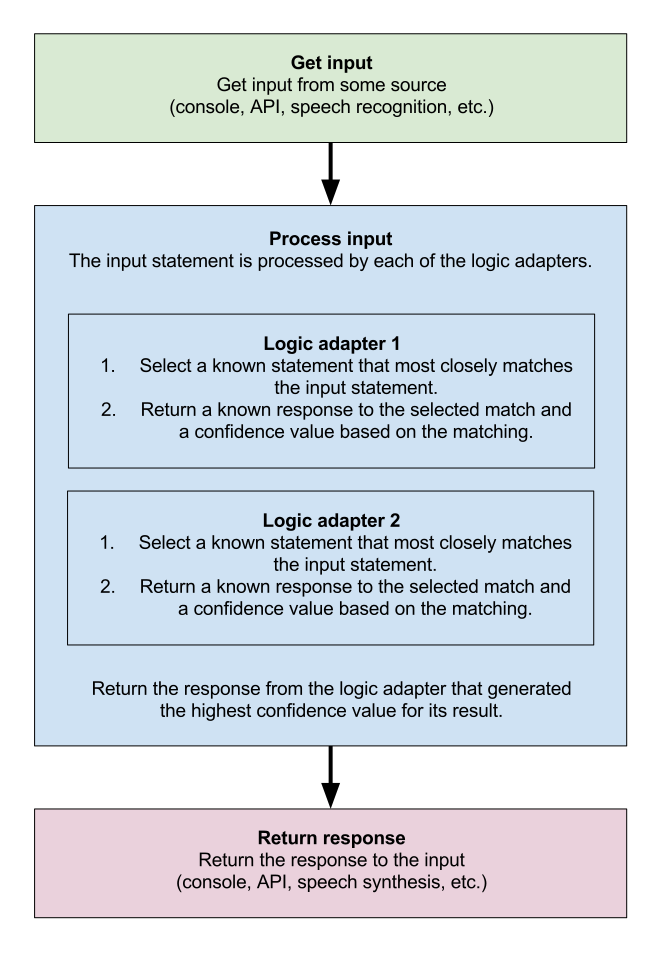
\includegraphics[width=0.8\columnwidth]{chatterbot-process-flow}%
    \caption{\captionstyle{Process flow diagram of how Chatterbot works on a higher level \cite{Chatterbot:online}}}%
    \label{fig:chatterbot-process-flow}%
\end{figure}

Firstly, the user inputs a statement. The statement is then processed by \textit{logic adapters}. A logic adapter is a function which takes text as input, determines whether it can process the input, and generates suitable output.

The main advantage of Chatterbot is its extensibility. While it provides a lot of built-in functionality, it might not be suitable for all projects.

[Add a figure showing how it works in more detail here...]

\myparagraph{Configuration}
Chatterbot provides a \textit{ChatBot} class. A ChatBot object takes several parameters in its constructor which define its behaviour:
\begin{itemize}
    \item \texttt{preprocessors}
    \item \texttt{logic\_adapters}
    \item \texttt{storage\_adapters}
\end{itemize}

\myparagraph{Preprocessors}
The ChatBot instance can take a list of functions in its constructor to be used as preprocessors. Preprocessors can modify the input sent by the user before it is passed to the logic adapters. This is necessary due to the fact that the logic adapters are more likely to perform better if they are given "clean" input. For example, if the input contains a lot of whitespaces or non-alphanumerical characters, it might be beneficial to remove them. Chatterbot has several preprocessors, however, custom functions can be created and used as preprocessors.

\myparagraph{Logic Adapters}
\textit{Logic adapters} are used to select an appropriate response to a question entered by the user. More than one logic adapter may be used as different types of input may require different processing. For example, Chatterbot by default uses the \textit{BestMatch} logic adapter. However, this adapter is only useful when the question asked has a specific response. If the user asked for the current time, the BestMatch adapter would be unable to answer as there is no specific answer to this question, i.e. the answer changes depending on when the user asks the question. For this reason, a \textit{Time} logic adapter can be created and added to the list of adapters used (Chatterbot has this adapter implemented by default). To help decide which adapter to use if more than one are provided, a custom logic adapter must inherit from the base class \texttt{LogicAdapter} and must implement the method \texttt{can\_process()}. This method is called before the logic adapters generate a response and the user input is passed to it. It must then return True or False based on whether the adapter should process this input or not. \cref{lst:canprocess} shows an example implementation of the \texttt{can\_process} method.

\begin{lstlisting}[caption={\small{\textit{Example implementation of the can\_process method. Adapted from \cite{Chatterbot:online}}}}, label={lst:canprocess}]
    def can_process(self, statement):
        # If the statements starts with
        # the string 'Hey John',
        if statement.text.startswith('Hey John')
            # it can be processed with this adapter
            return True
        # If not,
        else:
            # it can't
            return False
\end{lstlisting}

This tells the adapter to only process user input which contains the string "Hey John" (John could be the name of the chatbot) in its beginning.

Another requirement is that custom logic adapters implement the \texttt{process()} method. It takes the input statement as a parameter. Additional response selection parameters can be added if required by the application. An example implementation can be seen in \cref{lst:process}.

\begin{lstlisting}[caption={\small{\textit{Example implementation of the process() method. Adapted from \cite{Chatterbot:online}}}}, label={lst:process}]
    def process(self, input_statement, additional_response_selection_parameters):
        import random

        # Randomly select a confidence
        # value between 0 and 1
        confidence = random.uniform(0, 1)

        # For this example,
        # the input will just be returned
        # as output
        selected_statement = input_statement
        selected_statement.confidence = confidence

        return selected_statement
\end{lstlisting}

The \texttt{process()} method must return a \textit{Statement} object. The \textit{text} property of the object should contain the actual response to the input. Additionally, the \textit{confidence} property should be a value between 0 and 1 which indicates how confident the adapter is that this response is correct. In the example above, the text of the output statement is set to the same text that was entered by the user. The confidence value is chosen randomly and the response is returned.

In the event that more than one logic adapters are used, and more than one of them returns a response, the response with the highest value of confidence is selected. If two or more responses have the same value of confidence, then the response of the adapter which is first in the list of adapters is used. \cref{fig:dialog-processing-flow} shows a diagram of response selection with multiple adapters.

\begin{figure}[!htb]%
    \centering
    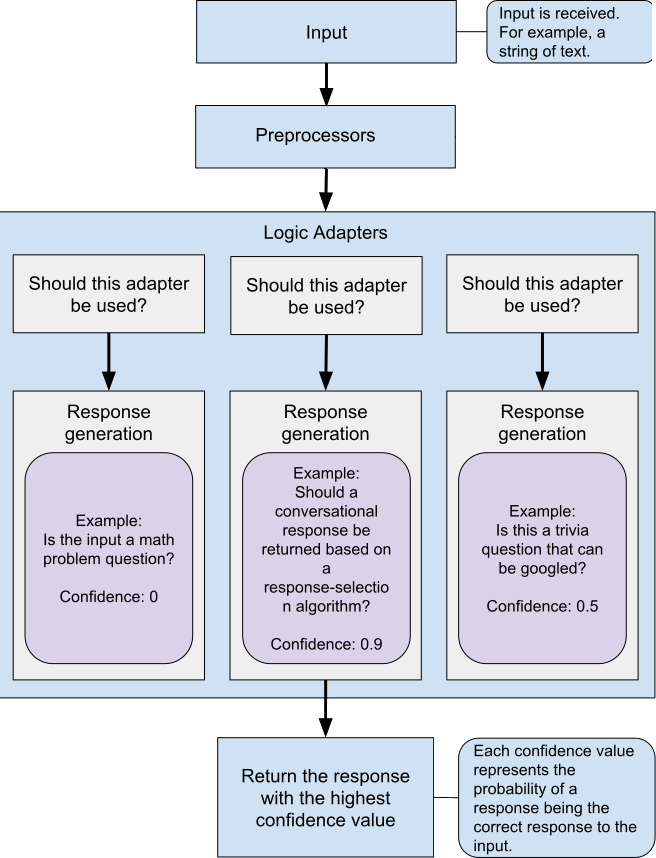
\includegraphics[width=0.7\columnwidth]{dialog-processing-flow}%
    \caption{\captionstyle{Process flow diagram of how responses are selected. Adapted from \cite{Chatterbot:online}}}%
    \label{fig:dialog-processing-flow}%
\end{figure}


By default, Chatterbot has the following adapters included:
\begin{itemize}
    \item Best Match Adapter - used when question that have a specific response are asked. This requires training data and the quality of the response depends on the quality of the training data. The adapter uses a specific \textit{similarity} function to search through the known questions. When it finds the most similar one, it then returns the known response to this question. The similarity functions available by default are:
        \begin{itemize}
            \item Levenshtein Distance - this method is used by default...
            \item Jaccard Similarity - ...
            \item Sentiment Comparison - ...
            \item Synset Distance - ...
            \item Custom similarity functions may be implemented if needed.
        \end{itemize}
    \item Time Logic Adapter - allows the user to ask about the current time.
    \item Mathematical Evaluation Adapter - calculates mathematical expression the user has entered.
    \item Specific Response Adapter - returns a specific predefined answer to a specific statement configured in the adapter.
\end{itemize}

\myparagraph{Storage Adapters}
\textit{Storage Adapters} are an interface for Chatterbot to connect to different storage technologies \cite{Chatterbot:online}. The storage adapter used by default is the \textit{SQL Storage Adapter}. It allows the chatbot to store its data in a local \textit{sqlite} relational database. The structure of the database can be seen in \cref{fig:db-schema}.

\begin{figure}[!htb]%
    \centering
    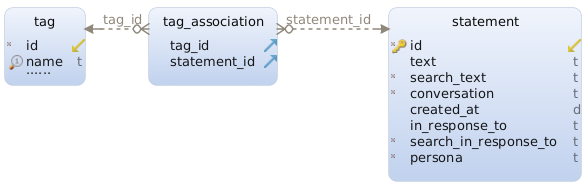
\includegraphics[width=0.9\columnwidth]{db-schema}%
    \caption{\captionstyle{Diagram of the database schema.}}%
    \label{fig:db-schema}%
\end{figure}

[Explain the structure here....]

\myparagraph{Training}
ChatterBot includes tools that help simplify the process of training a chatbot instance. ChatterBot’s training process involves loading example dialogue into the chatbot’s database. This either creates or builds upon the graph data structure that represents the sets of known statements and responses. When a chat bot trainer is provided with a data set, it creates the necessary entries in the chatbot’s knowledge graph so that the statement inputs and responses are correctly represented. An example of this can be seen in \cref{fig:training-graph}.

\begin{figure}[!htb]%
    \centering
    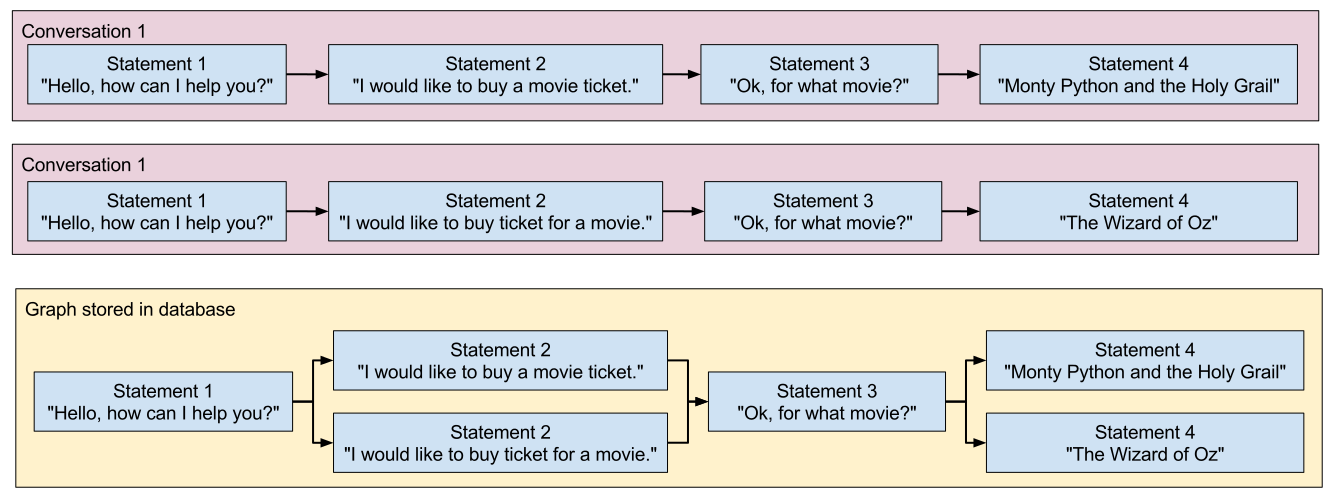
\includegraphics[width=1.0\columnwidth]{training-graph}%
    \caption{\captionstyle{Example of a training graph \cite{Chatterbot:online}.}}%
    \label{fig:training-graph}%
\end{figure}

[talk about how words are tagged with nltk here]

Chatterbot includes the following training clasess by default:
\begin{itemize}
    \item List Trainer - allows a chat bot to be trained using a list of strings where the list represents a conversation.
    \item Corpus Trainer - allows the chat bot to be trained using corpus data stored in an external file.
    \item Ubuntu Corpus Trainer - allows chatbots to be trained with the data from the Ubuntu Dialogue Corpus.
\end{itemize}

New training classes may be created and used to train a chatbot. The custom trainer must inherit from the \textit{Trainer} class and must implement the methods \texttt{train()} which can accept any arguments.

\myparagraph{Statements}
ChatterBot’s statement objects represent either an input statement that the chat bot has received from a user, or an output statement that the chat bot has returned based on some input.

ChatterBot stores knowledge of conversations as statements. Each statement can have any number of possible responses.

\begin{figure}[!htb]%
    \centering
    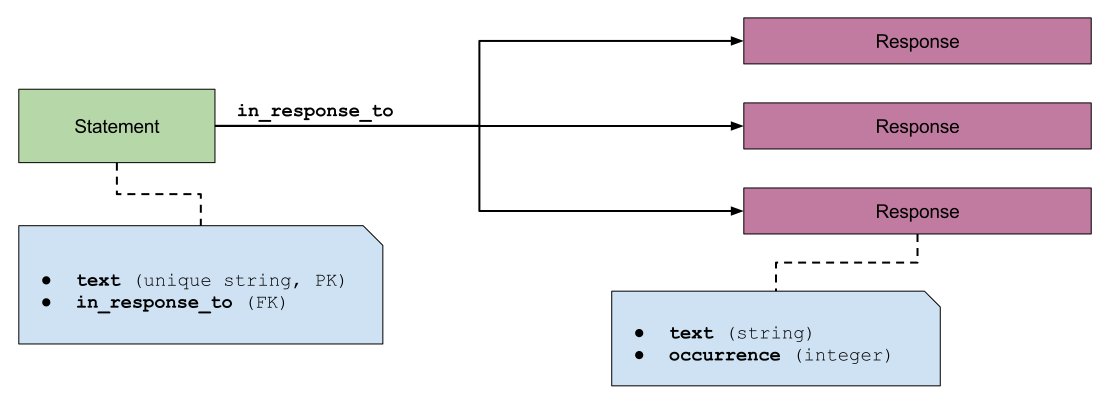
\includegraphics[width=1.0\columnwidth]{statement-response-relationship}%
    \caption{\captionstyle{Statement-response relationship \cite{Chatterbot:online}.}}%
    \label{fig:statement-response-relationship}%
\end{figure}

Each Statement object has an in\_response\_to reference which links the statement to a number of other statements that it has been learned to be in response to. The in\_response\_to attribute is essentially a reference to all parent statements of the current statement.

\begin{figure}[!htb]%
    \centering
    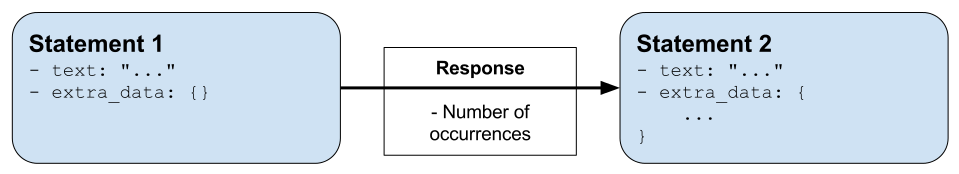
\includegraphics[width=1.0\columnwidth]{statement-relationship}%
    \caption{\captionstyle{Statement relationship \cite{Chatterbot:online}.}}%
    \label{fig:statement-relationship}%
\end{figure}

The count of recorded statements with matching, or similar text indicates the number of times that the statement has been given as a response. This makes it possible for the chat bot to determine if a particular response is more commonly used than another.

\subsubsection{Flask}
Flask is a microframework for Python used for website development. It is called a "microframework" as it aims to only include the core functionality required to create a website. This means developers are not forced to use a specific technology chosen for them by the Flask developers. Instead, many extensions exist which provide specific functionality. For instance, by default, Flask does not include any database....

Flask uses several python libraries to achieve its functionality. A description of each one is provided below:

\myparagraph{Werkzeug}
Werkzeug is a Python module used for creating \textit{WSGI} (Web Server Gateway Interface) applications. 

\myparagraph{Jinja}
Jinja is Python template engine. 

\subsubsection{Pytest}
Pytest is a unit test framework for Python...

\subsection{Implementation}
\subsubsection{Version control}
The first decision made when starting to implement the application was to use \textit{Version Control}. The version control system used was \textit{Git} and the code was hosted in a \textit{GitHub} repository. The reason for this was personal preference and previous experience with these technologies. 

Using Git and Github meant that the source code of the application could be easily shared between computers. Additionally, changes between versions of the program could be tracked. In the event that issues arose, the application could be reverted to a previous working version. 

Another feature of Git and Github used was \textit{branches}. Branches allow for having several versions of the code at the same time:
\begin{itemize}
    \item Master branch - stable version of the application which can be deployed.
    \item Dev branch - the most recent updates to the application which might not be fit for deployment. It can be updated until it is considered stable enough. It can then be merged into the master branch and deployed.
    \item Feature branches - a branch where a specific feature is implemented. It can then be merged into the development branch.
\end{itemize}

Using branching proved to be beneficial as... 

\subsubsection{Application}
Early in the development process it became clear that the application should consist of two main parts: the back-end and the front-end. The back-end program processes the user input and generates suitable output. The front-end is the program the user interacts with. It allows them to send a message to the chatbot and receive an answer.

\subsubsection{Back-end}
The back-end program consists of a web crawler and the chatbot program.

\myparagraph{Web crawler}
Firstly, before creating the back-end program, it was necessary to collect training data for the chatbot. This could be achieved in many different ways, however the decision to scrape \footnote{Web scraping - a technique for extracting data from a website.} the website Stack Overflow was ultimately made. Stack Overflow is one of the most popular websites where programmers can ask questions about numerous programming languages and technologies. Furthermore, there is a voting system which sorts the answers by number of votes. Additionally, the person who asks a question is able to mark a specific answer as the "accepted answer". This meant that when collecting data, the answers to each question could be sorted by number of votes, and the "accepted answer" could be used as the default answer. Unfortunately, some questions have no accepted answer or no answers at all. Despite that, Stack Overflow has a wealth of information and proved to be a good source.

Another option for data collection was the numerous websites which provide beginner information about a specific language. However, as described below, supporting web crawling of different websites could be a difficult task due to the different structure of each website. Furthermore, these websites had a limited amount of information and some of them had outdated or low-quality information.

The last consideration for data collection was using books as training data. There exist numerous books about programming and they contain detailed information about technologies. However, it was decided that using books was infeasible as the Chatterbot library required training data in the format question - answer. Converting a book to this format would require creating a another program which would possibly utilise NLP and other advanced machine learning techniques. This would be a difficult task and it would be outside of the scope of this project.

It was decided that data about the C++ programming language would be collected. C++ is widely used for programs where performance is most important such as games. However, it is known to have a steep learning curve....

A python program was written to collect data from Stack Overflow. The Python module \textit{BeautifulSoup} was utilised to achieve data extraction from the pages. The program expects the following variables to work:
\begin{itemize}
    \item Starting page - the first page to be crawled.
    \item Number of pages to be crawled
\end{itemize}

Initially, they were implemented as constants, however it was planned for them to be set with command line arguments later.

Another variable, \texttt{current\_page} (indicating the currently scraped page,) is initially set to the value of the starting page variable. Then a \texttt{while} loop is executed until the value of \texttt{current\_page} becomes the same as the value of \texttt{start + num\_pages}, where \texttt{start} is the starting page and \texttt{num\_pages} is the number of pages to be crawled. The value of \texttt{current\_page} is incremented by one at the end of each loop iteration. In the beginning of each loop iteration, a URL of the page to be scraped is generated. This is achieved by appending several \textit{GET} parameters to the base Stack Overflow URL. The structure of a Stack Overflow URL can be seen in \cref{fig:so-url}.

\begin{figure}[!htb]%
    \centering
    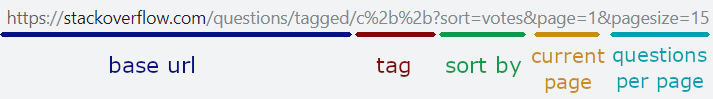
\includegraphics[width=1.0\columnwidth]{so-url}%
    \caption{\captionstyle{The structure of a Stack Overflow URL.}}%
    \label{fig:so-url}%
\end{figure}

The \textbf{base URL} is a constant value. The \textbf{tag}, \texttt{c\%2b\%2b}, is used to show only questions categorised under this tag. In this case, \textbf{C++} questions are requested as \texttt{\%2b} expands to the symbol \texttt{+}. However, the tag can be changed to any language or technology. For instance, to collect data about Java, the tag can be changed to \texttt{java} and this would result in only extracting data from Java-related questions. The \textbf{sort} parameter indicates the order in which the questions are shown. In this case sorting by \texttt{votes} results in the most upvoted questions being shown first. The \textbf{page} parameter indicates the current page. Since there is a large number of questions on the website, it is impossible to display them all in one page. For this reason, questions are split into pages. The last parameter used is \textbf{pagesize}. It indicates how many questions should be shown per page. To generate a URL, all the parameters are appended to the base URL, and the \textbf{page} parameter is dynamically generated based on the \texttt{current\_page} variable. 

With the generated URL, a \textit{request} can be sent to Stack Overflow. Using the Python library \textbf{requests}, a GET request can be sent. The returned result is the source code of the page that the request was sent to. Data can now be extracted from the source code using the \textit{Beautiful Soup} Python library. Firstly, an instance of the \texttt{BeautifulSoup} class is created. The source code retrieved earlier is passed to it. The library can then parse the code and create a \textit{parse tree} from which data can be extracted. The data needed from each page of questions is the hyperlink to each question's page. To extract this data, the method \texttt{find\_all()} of the \texttt{BeautifulSoup} object can be used. It returns a list of all the occurrences of a specified HTML tag as a parameter. In this case, the HTML \texttt{<a>} tag is needed as it is used to create hyperlinks. However, there are numerous hyperlinks on each Stack Overflow page. Only the hyperlinks which lead to a question page are needed. Using the Chrome browser developer tools, it was discovered that each link to a question was assigned a class of "question-hyperlink". \cref{lst:hyperlink} shows the code of an example hyperlink to a question.

\begin{lstlisting}[language=html, caption={\captionstyle{An example hyperlink to a Stack Overflow question.}}, label={lst:hyperlink}]
    <a href="/questions/121162/what-does-the-explicit-keyword-mean" class="question-hyperlink">What does the explicit keyword mean?</a>
\end{lstlisting}

With this information, only the URLs of the questions could be extracted. \cref{lst:extract-questions} shows the source code for extracting the hyperlinks to each question.

\begin{lstlisting}[caption={\captionstyle{Extracting the URL of each question on a Stack Overflow page.}}, label={lst:extract-questions}]
    # get a link to each question
    for ques_link in soup.find_all('a', {'class': 'question-hyperlink'}):
        # make sure no extra links are crawled
        if q_no == PAGE_SIZE:
            break
        # generate the link
        url = SO_URL + ques_link.get('href')
        # print question title for debugging purposes
        title = ques_link.get_text()
        if VERBOSE_OUTPUT is True:
            print(title)
        # parse this question
        parse_question(url, title, data)
        # keep track of current question number
        q_no += 1
\end{lstlisting}

The \texttt{find\_all()} method on line 3 returns a list of all \texttt{<a>} tags with a class parameter set to "question-hyperlink". A for-each loop iterates through this list. Each hyperlink's destination is extracted from the \texttt{href} parameter using the \texttt{get()} method. Each link's text is also extracted using the \texttt{get\_text()} method. The destination URl, however, is incomplete and it needs to be appended to the base Stack Overflow URL. The final question URL and the question title are passed to the \texttt{parse\_question()} method. The if-statement on line 4 is needed as there is a "Hot Network Questions" section on each Stack Overflow page which contains hyperlinks to popular questions. The if statement ensures that only the required number of question links are scraped.

The \texttt{parse\_question()} method can be seen in \cref{lst:extract-answers}.
\begin{lstlisting}[caption={\captionstyle{Extracting answers for a specific Stack Overflow question.}}, label={lst:extract-answers}]
    def parse_question(url, title, data):
    # page to be scraped
    page = requests.get(url, headers=headers, timeout=(3, 30))
    # initialise bs4
    soup = BeautifulSoup(page.content, 'lxml')
    # get the question data, contained in a <div> with class "postcell"
    question = soup.find('div', class_='postcell')
    if question is not None:
        answers = soup.find_all('div', class_='answercell')
        # limit to max 3 answers per question
        end = len(answers)
        if end > CRAWLER_NUM_ANSWERS:
            end = CRAWLER_NUM_ANSWERS
        # for each answer found
        for i in range(0, end):
            # get the answer text
            answer = answers[i].find('div', class_='post-text').extract()
            # store the question and the answer in their own list
            answer = str(answer)
            entry = [title, answer]
            # add to the main list
            data.append(entry)
\end{lstlisting}

The \textit{requests} library is used again to send a GET request to each of the question pages. The returned source code is then passed to an instance of \texttt{BeautifulSoup}. Using the Chrome browser's development tools it was discovered that the data about a question is stored in a HTML \texttt{<div>} with a class value "postcell". However this includes all data including the date the question was asked, the author, etc. The actual text of the post is stored in a \texttt{div} with class value "post-text". Each answer is stored in a \texttt{<div>} with class value "answercell". The actual text of the answer is stored in a \texttt{<div>} with class value "post-text". With this information, the answers to each question can be extracted by first finding them with the \texttt{find\_all() method}. The resulting list is then iterated through and each answer's text is extracted. The maximum number of answers scraped is currently set to three. However, the if statement on line 12 ensures that in the event that less than three answers exist, no errors occur. Lastly, the question title and the top three answers are stored in a Python \textit{dict}.

The last step is to save the data stored in the dict to a file. The ChatterBot library supports training from external files by default. Custom trainers can be created to support different file formats, however the \textit{YAML} format which is supported by default can be used. The structure of a training file can be seen in \cref{fig:yaml-train}. 

\begin{figure}[!htb]%
    \centering
    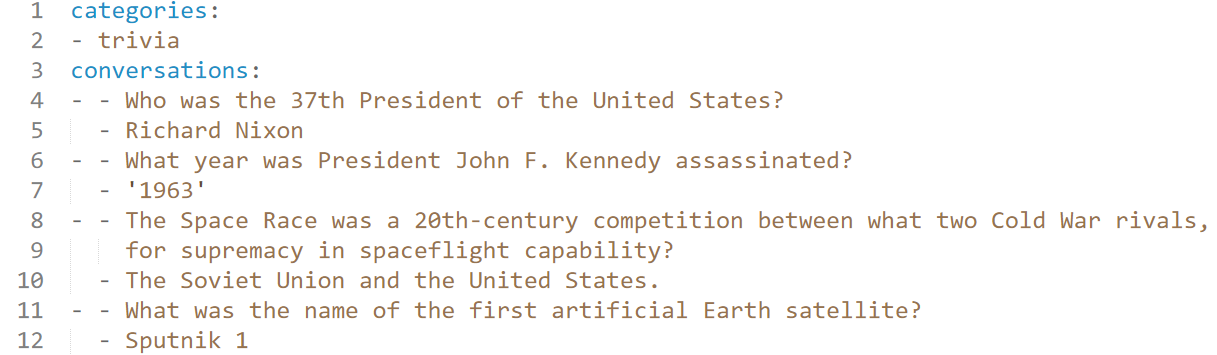
\includegraphics[width=1.0\columnwidth]{yaml-train}%
    \caption{\captionstyle{Example training file in the YAML format.}}%
    \label{fig:yaml-train}%
\end{figure}

The "\verb|- -|" tag is used to signify a statement, while the "\verb|-|" tag signifies an answer to a statement. To save the data collected from Stack Overflow in this format, the \textit{Ruamel.YAML} Python library was used. To ensure the data was saved in this required format, however, it had to first be stored in an appropriate data structure. Each question - answer pair was stored in a Python list. Each list was appended to a Python dict. Using the Ruamel.YAML library's \texttt{yaml} class, the data could be simply written to a file using the \texttt{yaml.dump()} method. The code used to achieve this can be seen in \cref{lst:write-file}.

\begin{lstlisting}[caption={\captionstyle{Writing scraped data to a file in the YAML format.}}, label={lst:write-file}]
    # initialise yaml library
    yaml = YAML()
    yaml.default_flow_style = False
    # create output file
    out_file = os.path.join(DATA_DIR_PATH, "training_data.yaml")
    # open out file
    with open(out_file, 'w+', encoding="utf-8") as outfile:
        # write data
        yaml.dump(final_data, outfile)    
\end{lstlisting}

Even though the resulting program worked well, it was slow as only one question was processed at a time. To improve its performance, multithreading was implemented.

\begin{lstlisting}[caption={\captionstyle{Multithreaded optimisation of the web crawler.}}, label={lst:threads}]
    func = partial(crawl_pages, num_pages)
    try:
        with ThreadPoolExecutor(max_workers=workers) as executor:
            for i in range(workers):
                executor.submit(func, (i * num_pages + 1))
    except (KeyboardInterrupt, EOFError, SystemExit):
        print("Interrupted...")
\end{lstlisting}

\myparagraph{Chatbot}
The other main part of the back-end program is the Chatbot object instance. The initialisation of the chatbot can be seen in \cref{lst:chatbot}.

\begin{lstlisting}[caption={\captionstyle{Initialisation of the Chatbot object.}}, label={lst:chatbot}]
bot = ChatBot(
    "C++ bot",
    storage_adapter="chatterbot.storage.SQLStorageAdapter",
    preprocessors=[
        'chatterbot.preprocessors.unescape_html'
    ],
    logic_adapters=[
        {
            'import_path': 'chatbot.logic.BestMatch',
            'default_response': 'I am sorry, but I do not understand.',
            'maximum_similarity_threshold':  0.90
        }
    ]
)
\end{lstlisting}

The first argument passed to the constructor, the string "C++ bot", is the name of the chatbot. It can be useful when there are multiple chatbots created, however in this case there is only one chatbot instance. The second argument, \texttt{preprocessors} is a list of the preprocessors the chatbot should use when it receives user input. The \texttt{unescape\_html} preprocessor is included in chatterbot. It converts escaped HTML characters into unescaped HTMl characters. For instance, "\texttt{\&lt;b\&gt;}" is converted to the \texttt{<b>} tag. This preprocessor has to be used as the data collected from Stack Overflow includes HTML tags and some of them are escaped.

The next argument passed is a list \texttt{logic\_adapters}. The adapters used in this case are a BestMatch adapter and a SpecificResponse adapter.

The last argument is the \texttt{database\_uri}. An SQLite database is used and the value of the parameter is the name of the file where the database is stored.


\subsubsection{Front-end}
The front-end was implemented in Python with the Flask module.

\myparagraph{Project structure}
As suggested in the Flask documentation \cite{Flask:online}, the project was structured in the following way: 
\begin{verbatim}
Chatbot/
|---requirements.txt
|   
|---chatbot/
|   |---__init__.py
|   |---constants.py
|   |---crawler.py
|   |---bot.py
|   |   
|   |---static/
|   |   |---css/
|   |   |   |---style.css
|   |   |       
|   |   |---js/
|   |       |---chatbot.js
|   |           
|   |---templates/
|           |---base.html
|           |---chatbot.html
|           
|---tests/
|---venv/    
\end{verbatim}

The root folder of the project is the \texttt{Chatbot/} directory. It contains the \texttt{chatbot/} directory in which the Python code for the back-end program is stored. The \texttt{static/} directory contains the static files used in the website - the CSS styles and the javascript code as well as any images that might be used. The \texttt{tests/} directory contains the unit tests for the application. Lastly, \texttt{venv} contains the Python \textit{virtual environment} used for the project. Structuring the project this way ensures that the different .... are separated and organised.

\myparagraph{Application setup}
The Flask documentation recommends organising the code in modules. For this reason, the \texttt{\_\_init\_\_.py} file is placed in the \texttt{chatbot/} directory. This tells the Python interpreter that chatbot is a module which can be imported in Python files. Additionally, the \texttt{\_\_init\_\_.py} file defines a method which initialises an instance of the \texttt{Flask} class. This method is known as the \textit{Application Factory} \cite{Flask:online}. The initialisation of the Flask app is ahieved in the following way:

\begin{enumerate}
    \item An instance of the Flask class is created.
    \item The Flask instance is configured. A \texttt{SECRET\_KEY} variable is required by Flask. It is used to hash sensitive information in the website. During development, its value is set to the string "dev" so that debuggers can be used.
    \item The pages of the Flask application are initialised. For this project, the code for creating the home page can be seen in \cref{lst:homepage}. On line 1, the address of the page is specified. The "/" indicates that this is the home page. If a Contact page were to be added, its location would be "/contact". Line 2 defines a Python function which will be called when this address is accesed. Line 3 uses the Flask method \texttt{render\_template()}. It requires the name of an HTML file which will be shown when this page is accessed. The HTML file is stored in the \texttt{templates/} directory. This method takes any number of other optional arguments. Every other variable passed to it will be passed to the template specified and its value can be used via the Jinja templating language. In this case, a 'title' variable is passed which specifies the title that will be shown in the page.
    \item The last thing Flask requries is that the Application Factory returns the initialised and configured Flask object.
    \item The website can be run using the default server that comes with Flask. To do this, the command \texttt{flask run} can be executed from a terminal. Flask uses environment variables to locate a project. The variable \texttt{FLASK\_APP} must be set before running the server. To run the server in debug mode, the variable \texttt{FLASK\_ENV} may be set to "development". 
\end{enumerate}

\begin{lstlisting}[caption={\captionstyle{Initialisation of the home page of the Flask application.}}, label={lst:homepage}]
@app.route("/")
def home():
    return render_template("chatbot.html", title="Chatbot")
\end{lstlisting}

\myparagraph{Website design}
The website consists of a single page which resembles a text messaging application. The main goal was to create a clean and simple interface which is easy to use and feels familiar. Messaging apps such as Facebook Messenger and WhatsApp were used as reference. The website interface is shown in \cref{fig:site-interface}.

\begin{figure}[!htb]%
    \centering
    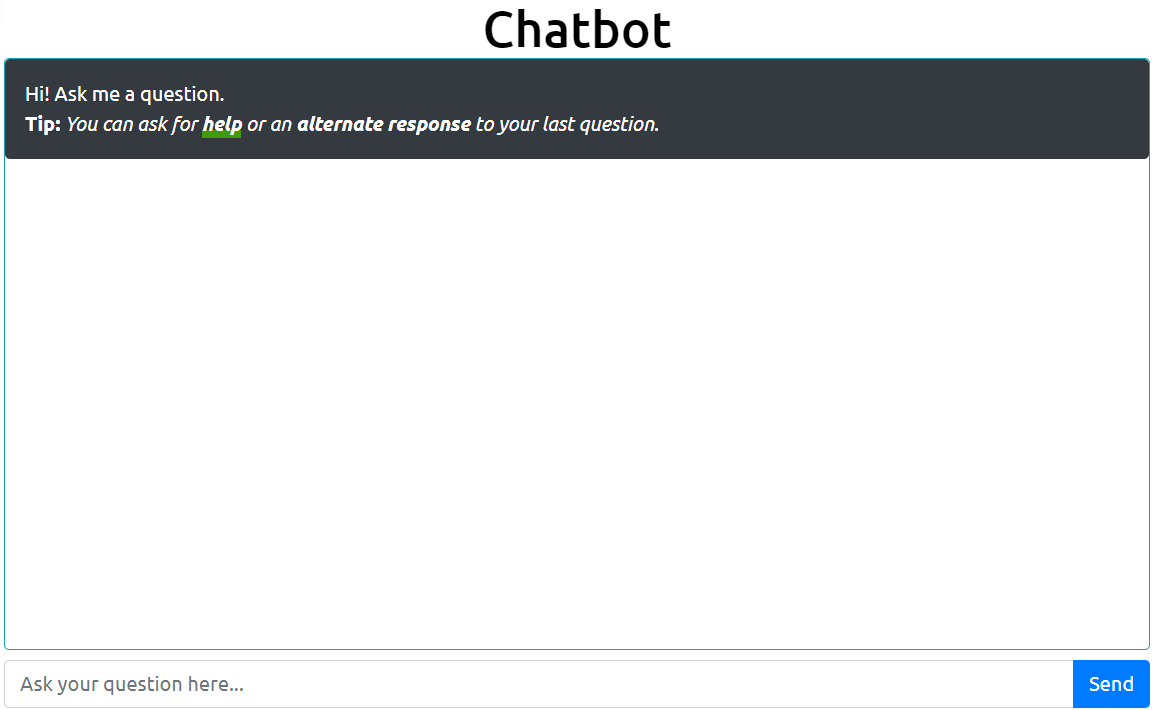
\includegraphics[width=1.0\columnwidth]{app-interface}%
    \caption{\captionstyle{The interface of the website.}}%
    \label{fig:site-interface}%
\end{figure}

The elements that can be seen on the figure were created using HTML and Jinja templates. A main template (\texttt{base.html}) contains the elements that exist on every page of the website - the page title and the window title. All the HTML code used to create a page is stored in - the <html>, <head>, and <body> tags. In its <head> tag all the css styles and javascript scripts are loaded. Additionally, the <title> tag is used with a value passed from Application Factory. The <body> tag only contains an HTML <h1> tag which has the value of the variable title passed from the Python code. The code used to achieve this can be seen in \cref{lst:jinjavar}. The code on line 1 checks if the variable \texttt{title} has a value. If it does, it is used on line 2 as a heading. There is no other content in the <body> tag, except for a Jinja block. It defines a place in the page where content can be inserted. This can be achieved by creating another template which extends the base template and implementing the block content in it.

\begin{lstlisting}[caption={\captionstyle{Using a variable passed from Python in a Jinja template.}}, label={lst:jinjavar}]

    <h1>{{ title }}</h1>

\end{lstlisting}

A specific template for the home page, \texttt{chatbot.html}, implements the elements specific to the chatbot page: the chatbox, the text field and the Submit button. It extends the \texttt{base.html} template. This means that all the code in the base template will be copied in the chatbot template. By defining a block with the same name as the block in the base template, the content of the chatbot page can be implemented.

The styling of the website was achieved using CSS. The CSS framework \textit{Bootstrap 4} by Twitter was used to style the website and to ensure that it can be viewed on devices with different screen sizes with no issues. Bootstrap's responsive design allows for positioning elements in a grid of rows and columns. Each row can contain up to twelve columns. When the page is resized, the columns are re-ordered and their size is changed dynamically to fit the page. The font size and can also change dynamically so that it. Although Bootstrap does not require any specific setup or configuration, the Flask extension Bootstrap-Flask can be used to simplify... It creates Jinja macros such as \texttt{bootstrap.load\_css()}, \texttt{bootstrap.load\_js()}, etc.

The chatbot page consists of three rows with one column per row. Custom CSS was written so that the different elements have appropriate size. The title is positioned at the top of the page and the text input box and the button are positioned at the bottom. The chatbox is in the center of the page and it occupies all the remaining free space. By default, Bootstrap uses rows with the same height. However, custom css was created to position the elements more precisely and to change their height. To ensure the responsive design still worked, the appropriate CSS units were used. Instead of giving elements a specific height, e.g. "20 pixels", relative units such as \texttt{\%} and \texttt{vh} were used.

\subsubsection{Communication between the front-end and the back-end}
The communication between the front-end and the back-end is required as the user input has to be sent to the back-end program for processing. When the input is processed, the resulting output has to be sent back to the front-end. This was achieved with \textit{Javascript}. 

Javascript is a client-side programming language which runs inside web browsers. It can be used to dynamically change a website's content, store information and handle requests and responses. The \textit{JQuery} library was used as it provides a simple and portable way of modifying content dynamically. Event handling, 

\subsubsection{Testing}
To ensure that after changing the back-end the other parts of the application worked correctly, a testing strategy was created. Unit tests were implemented with the Pytest python module. 

\myparagraph{Code Coverage}


\subsubsection{Continuous Integration \& Deployment}

\newpage
\section{Results and discussions}

\newpage
\section{Evaluation}

\newpage
\section{Conclusions}

\newpage
\section{Future work}

\newpage
\bibliographystyle{apalike}
\bibliography{./references}

%you can crate this on a extra tex document just like the title or any other part of the document.
\newpage
\begin{appendices}
\section{Project Overview}
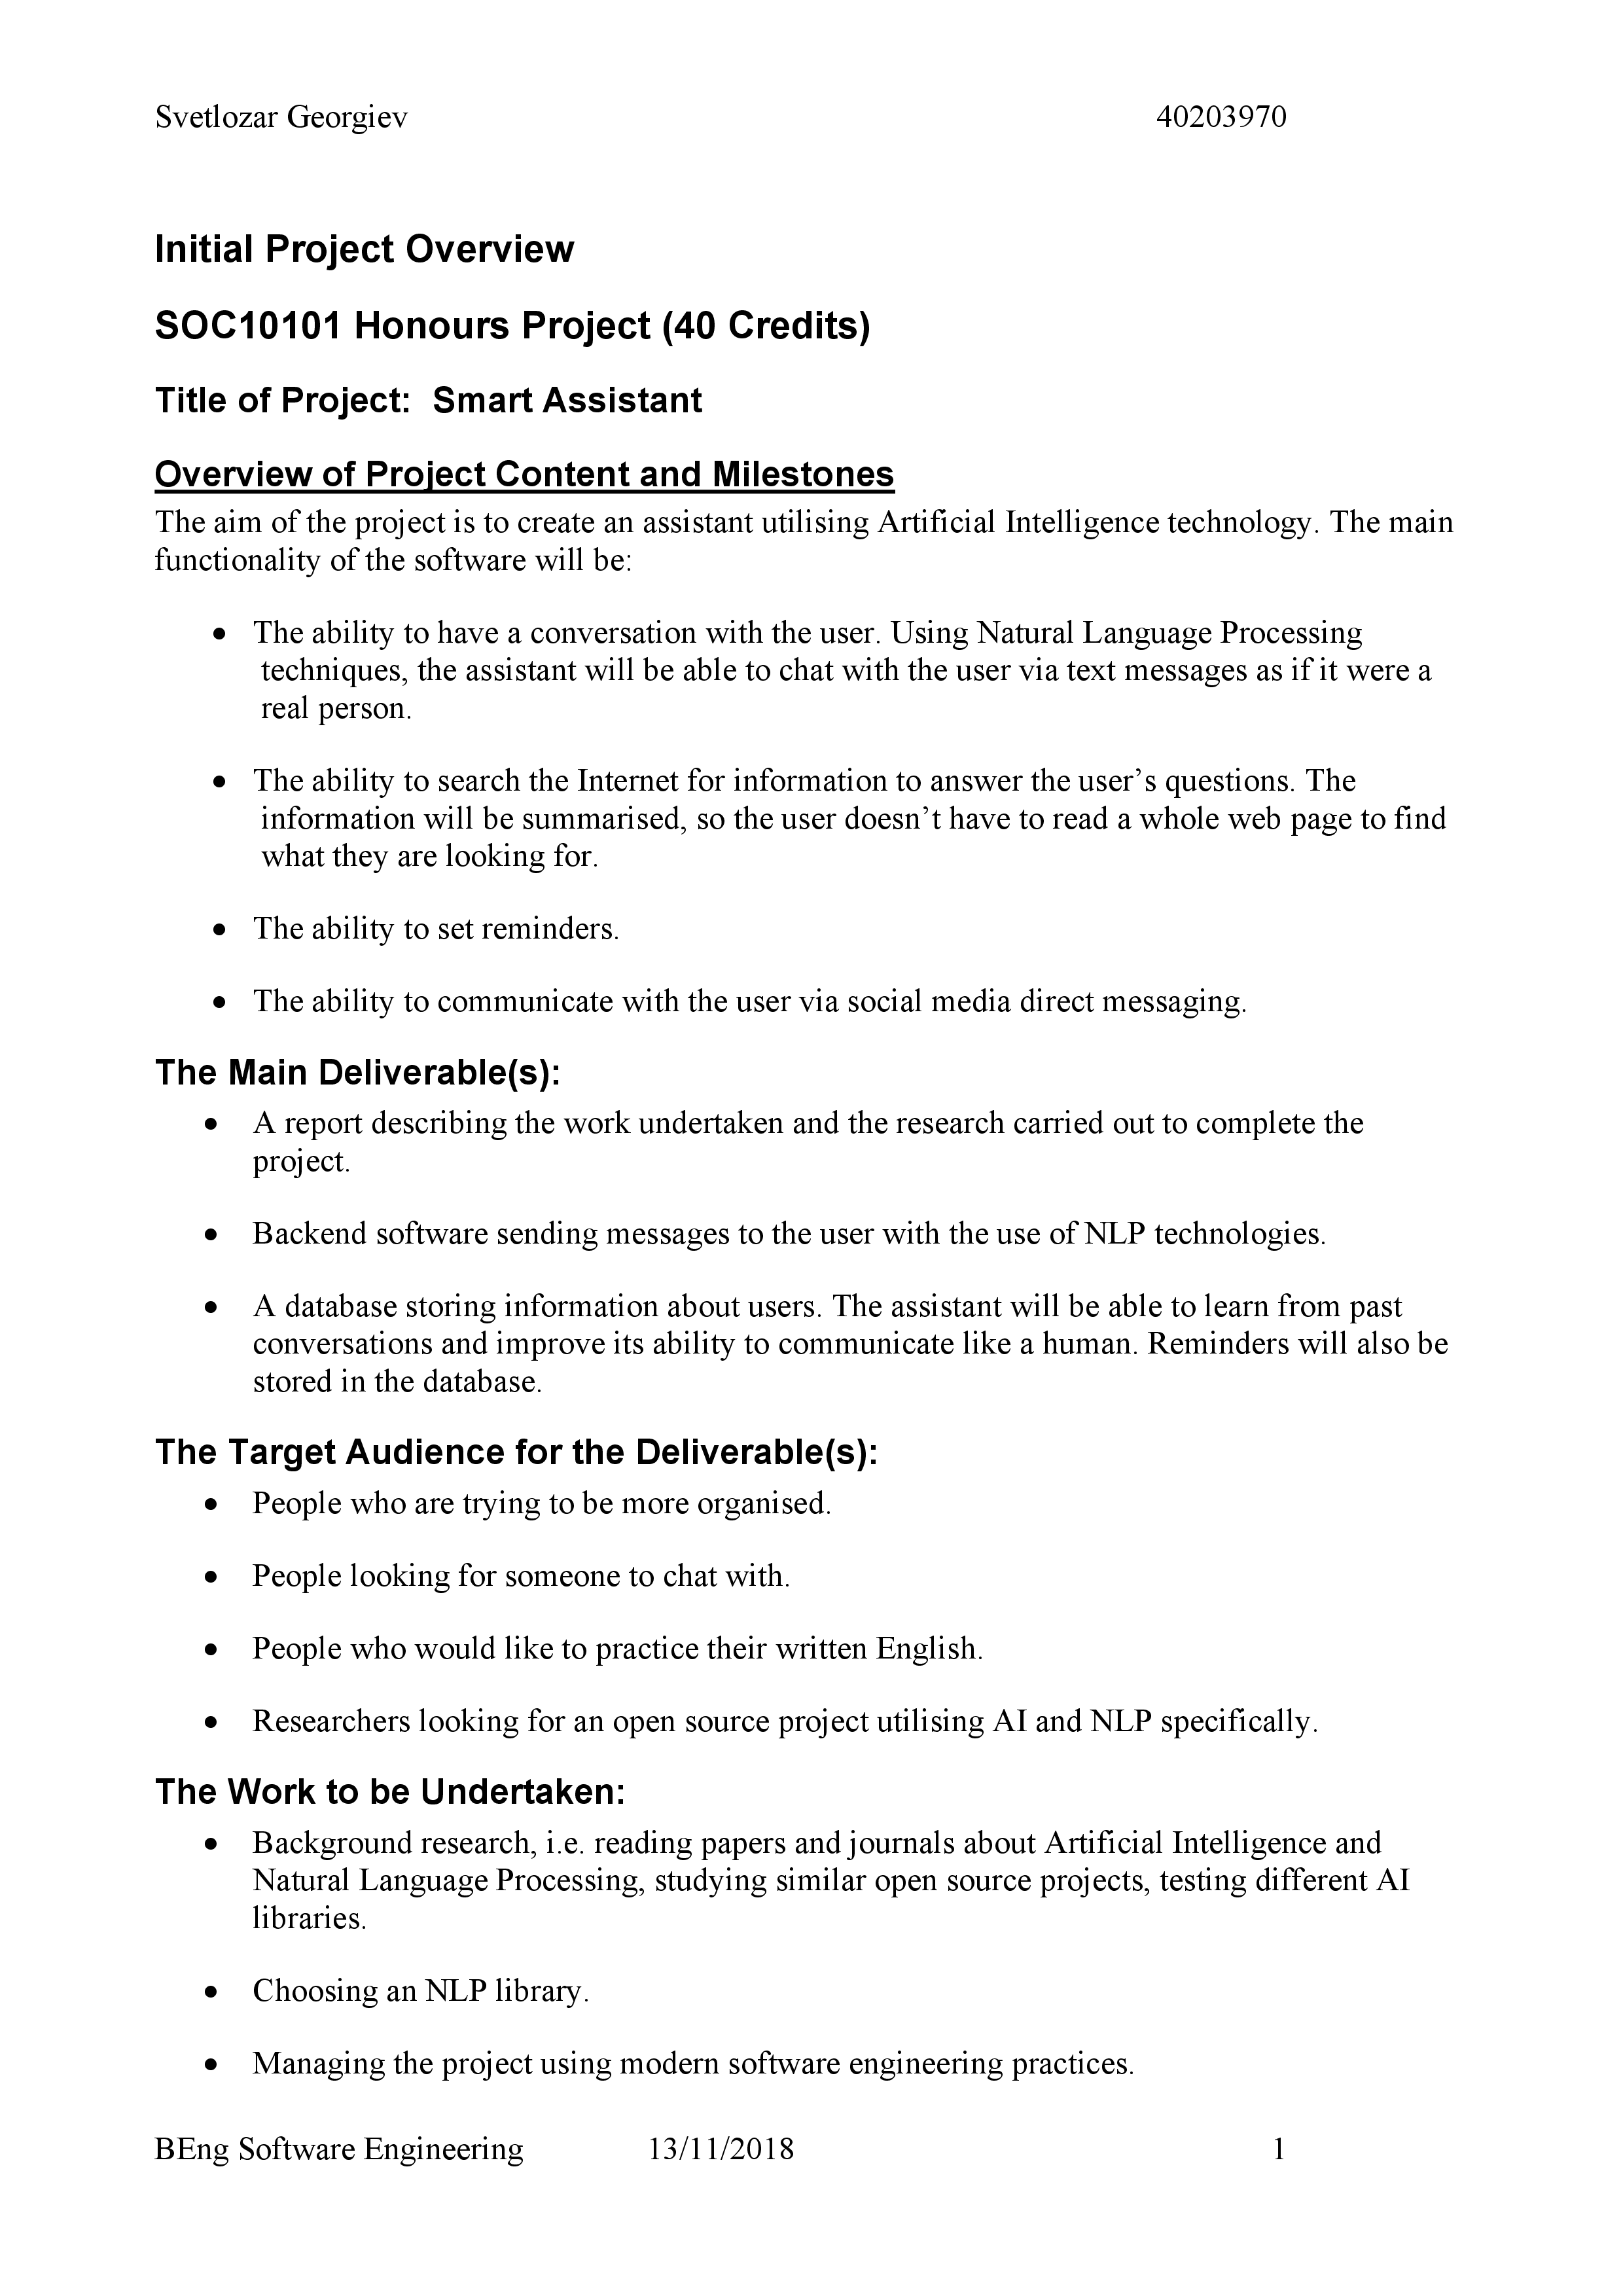
\includegraphics[width=\textwidth,height=\textheight,keepaspectratio]{IPO-0.png} % fit images to page
\newpage
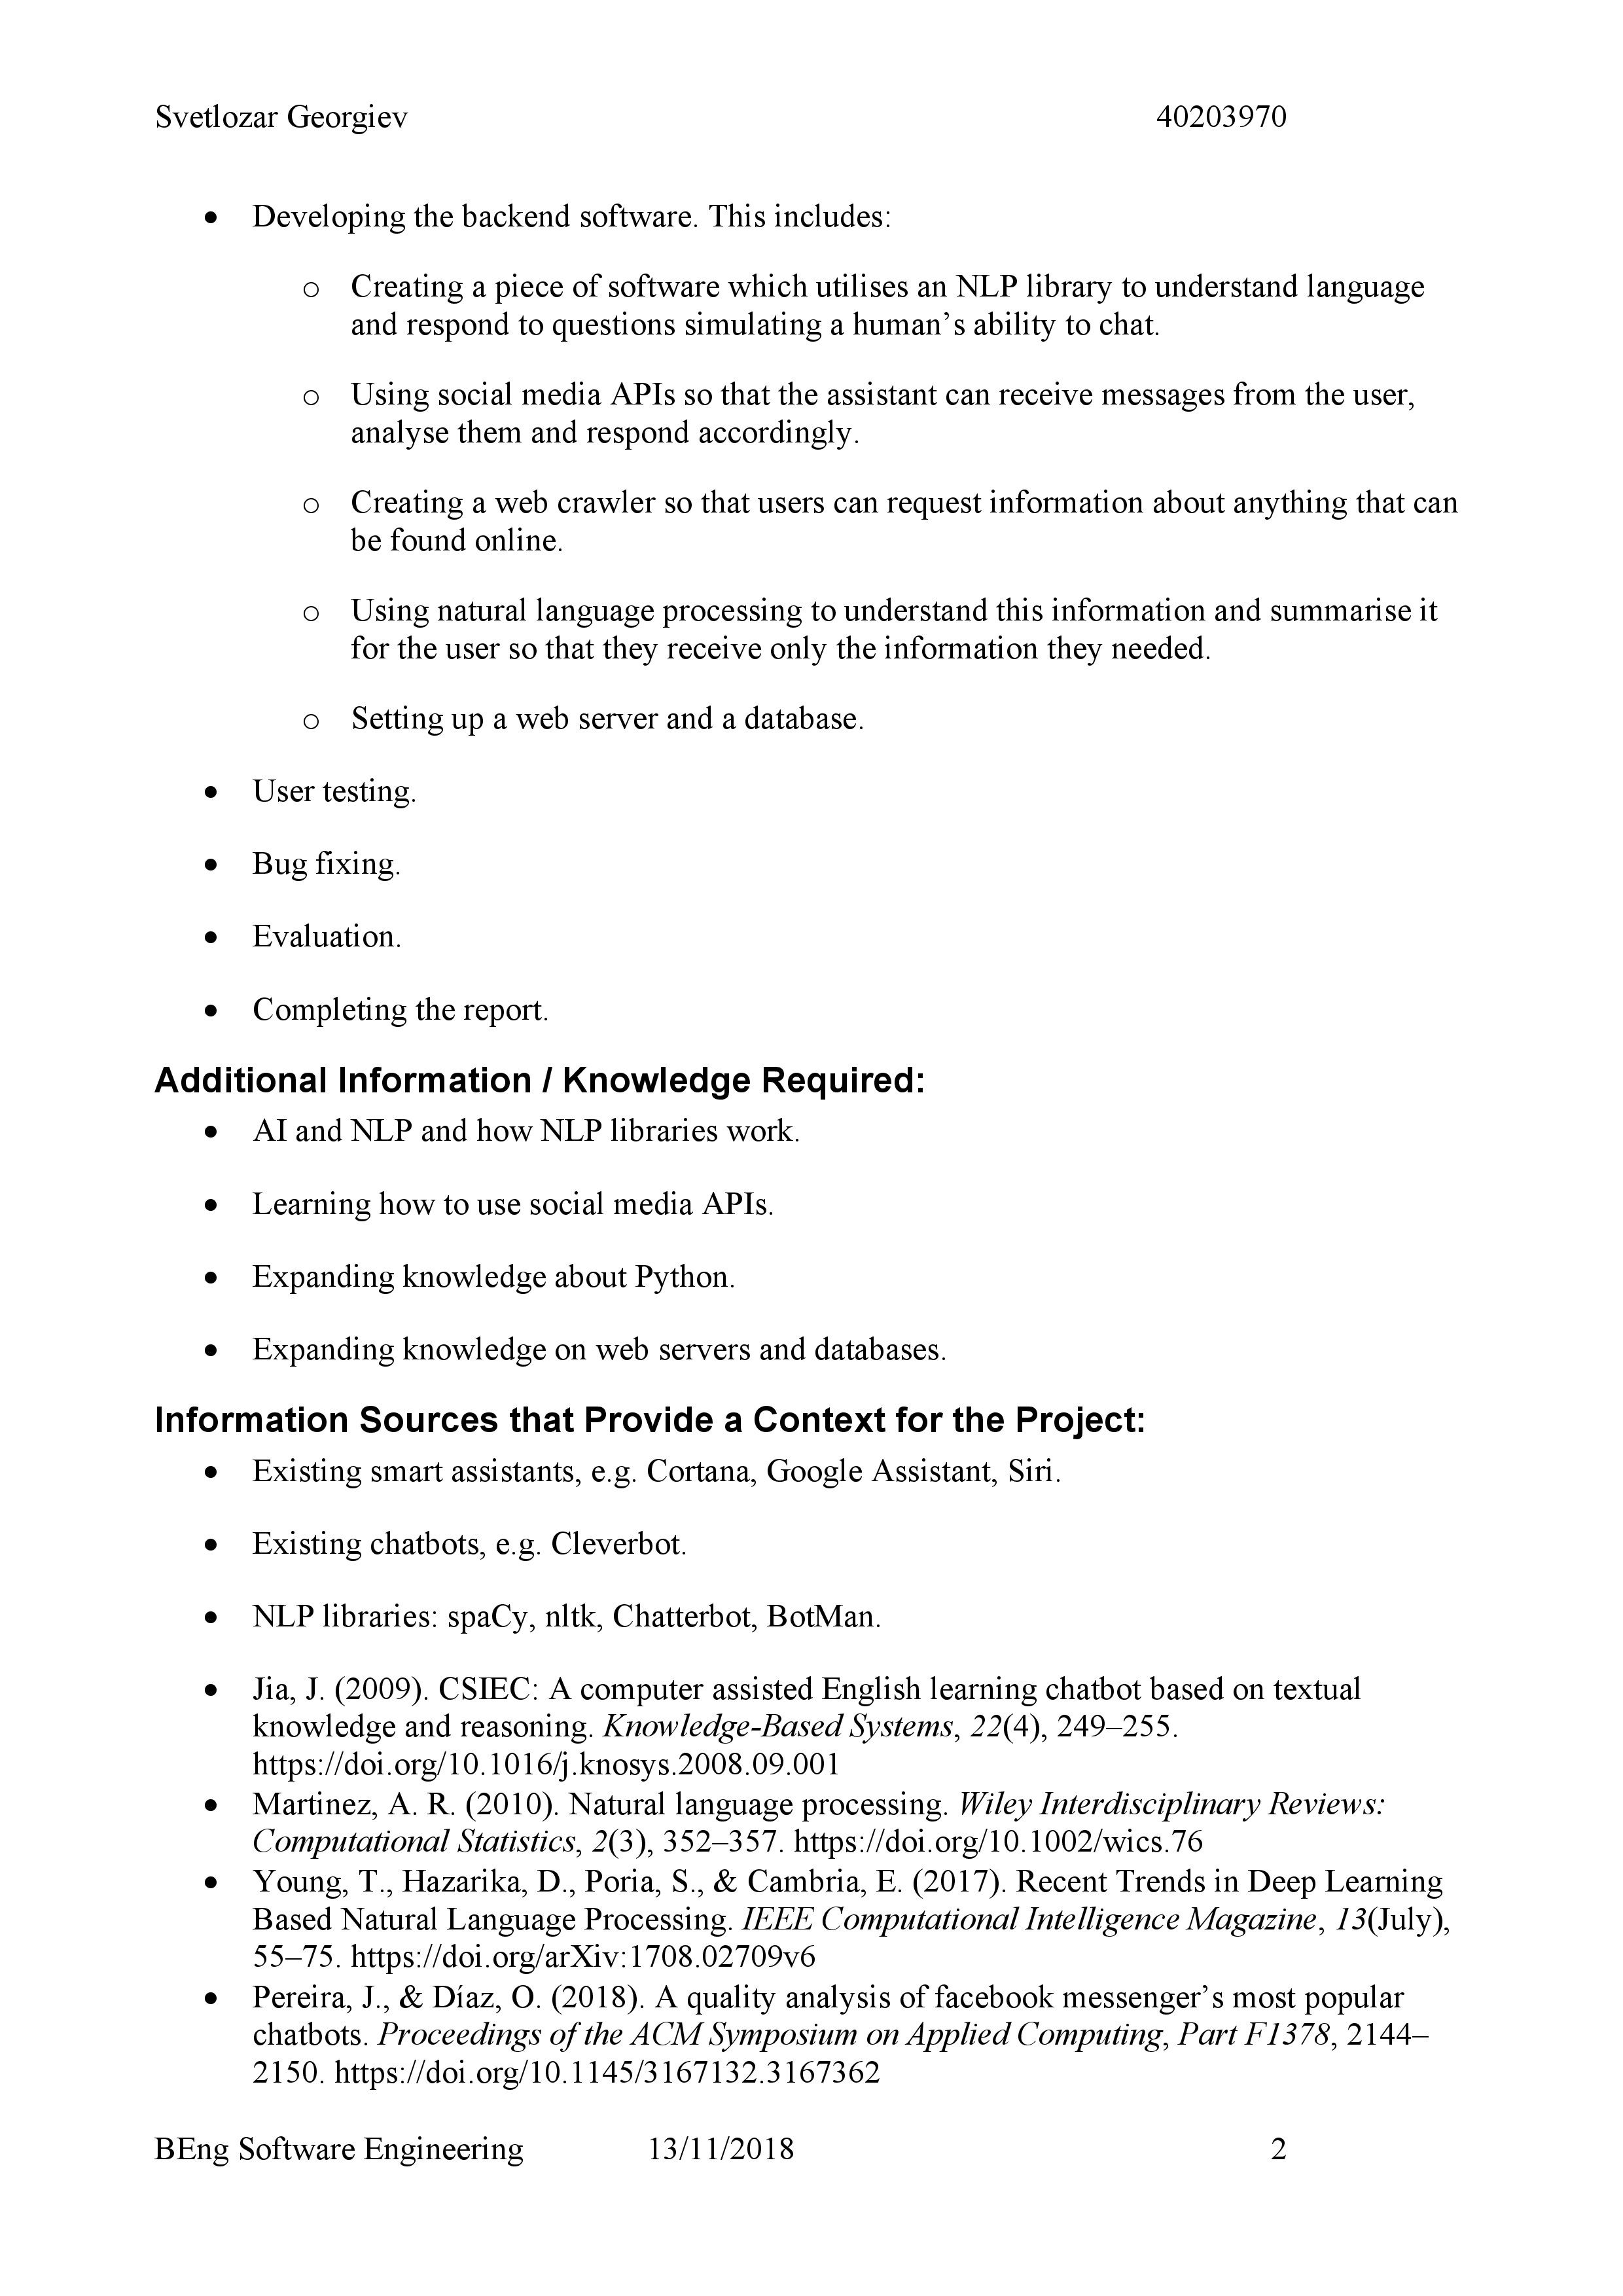
\includegraphics[width=\textwidth,height=\textheight,keepaspectratio]{IPO-1.png}
\newpage
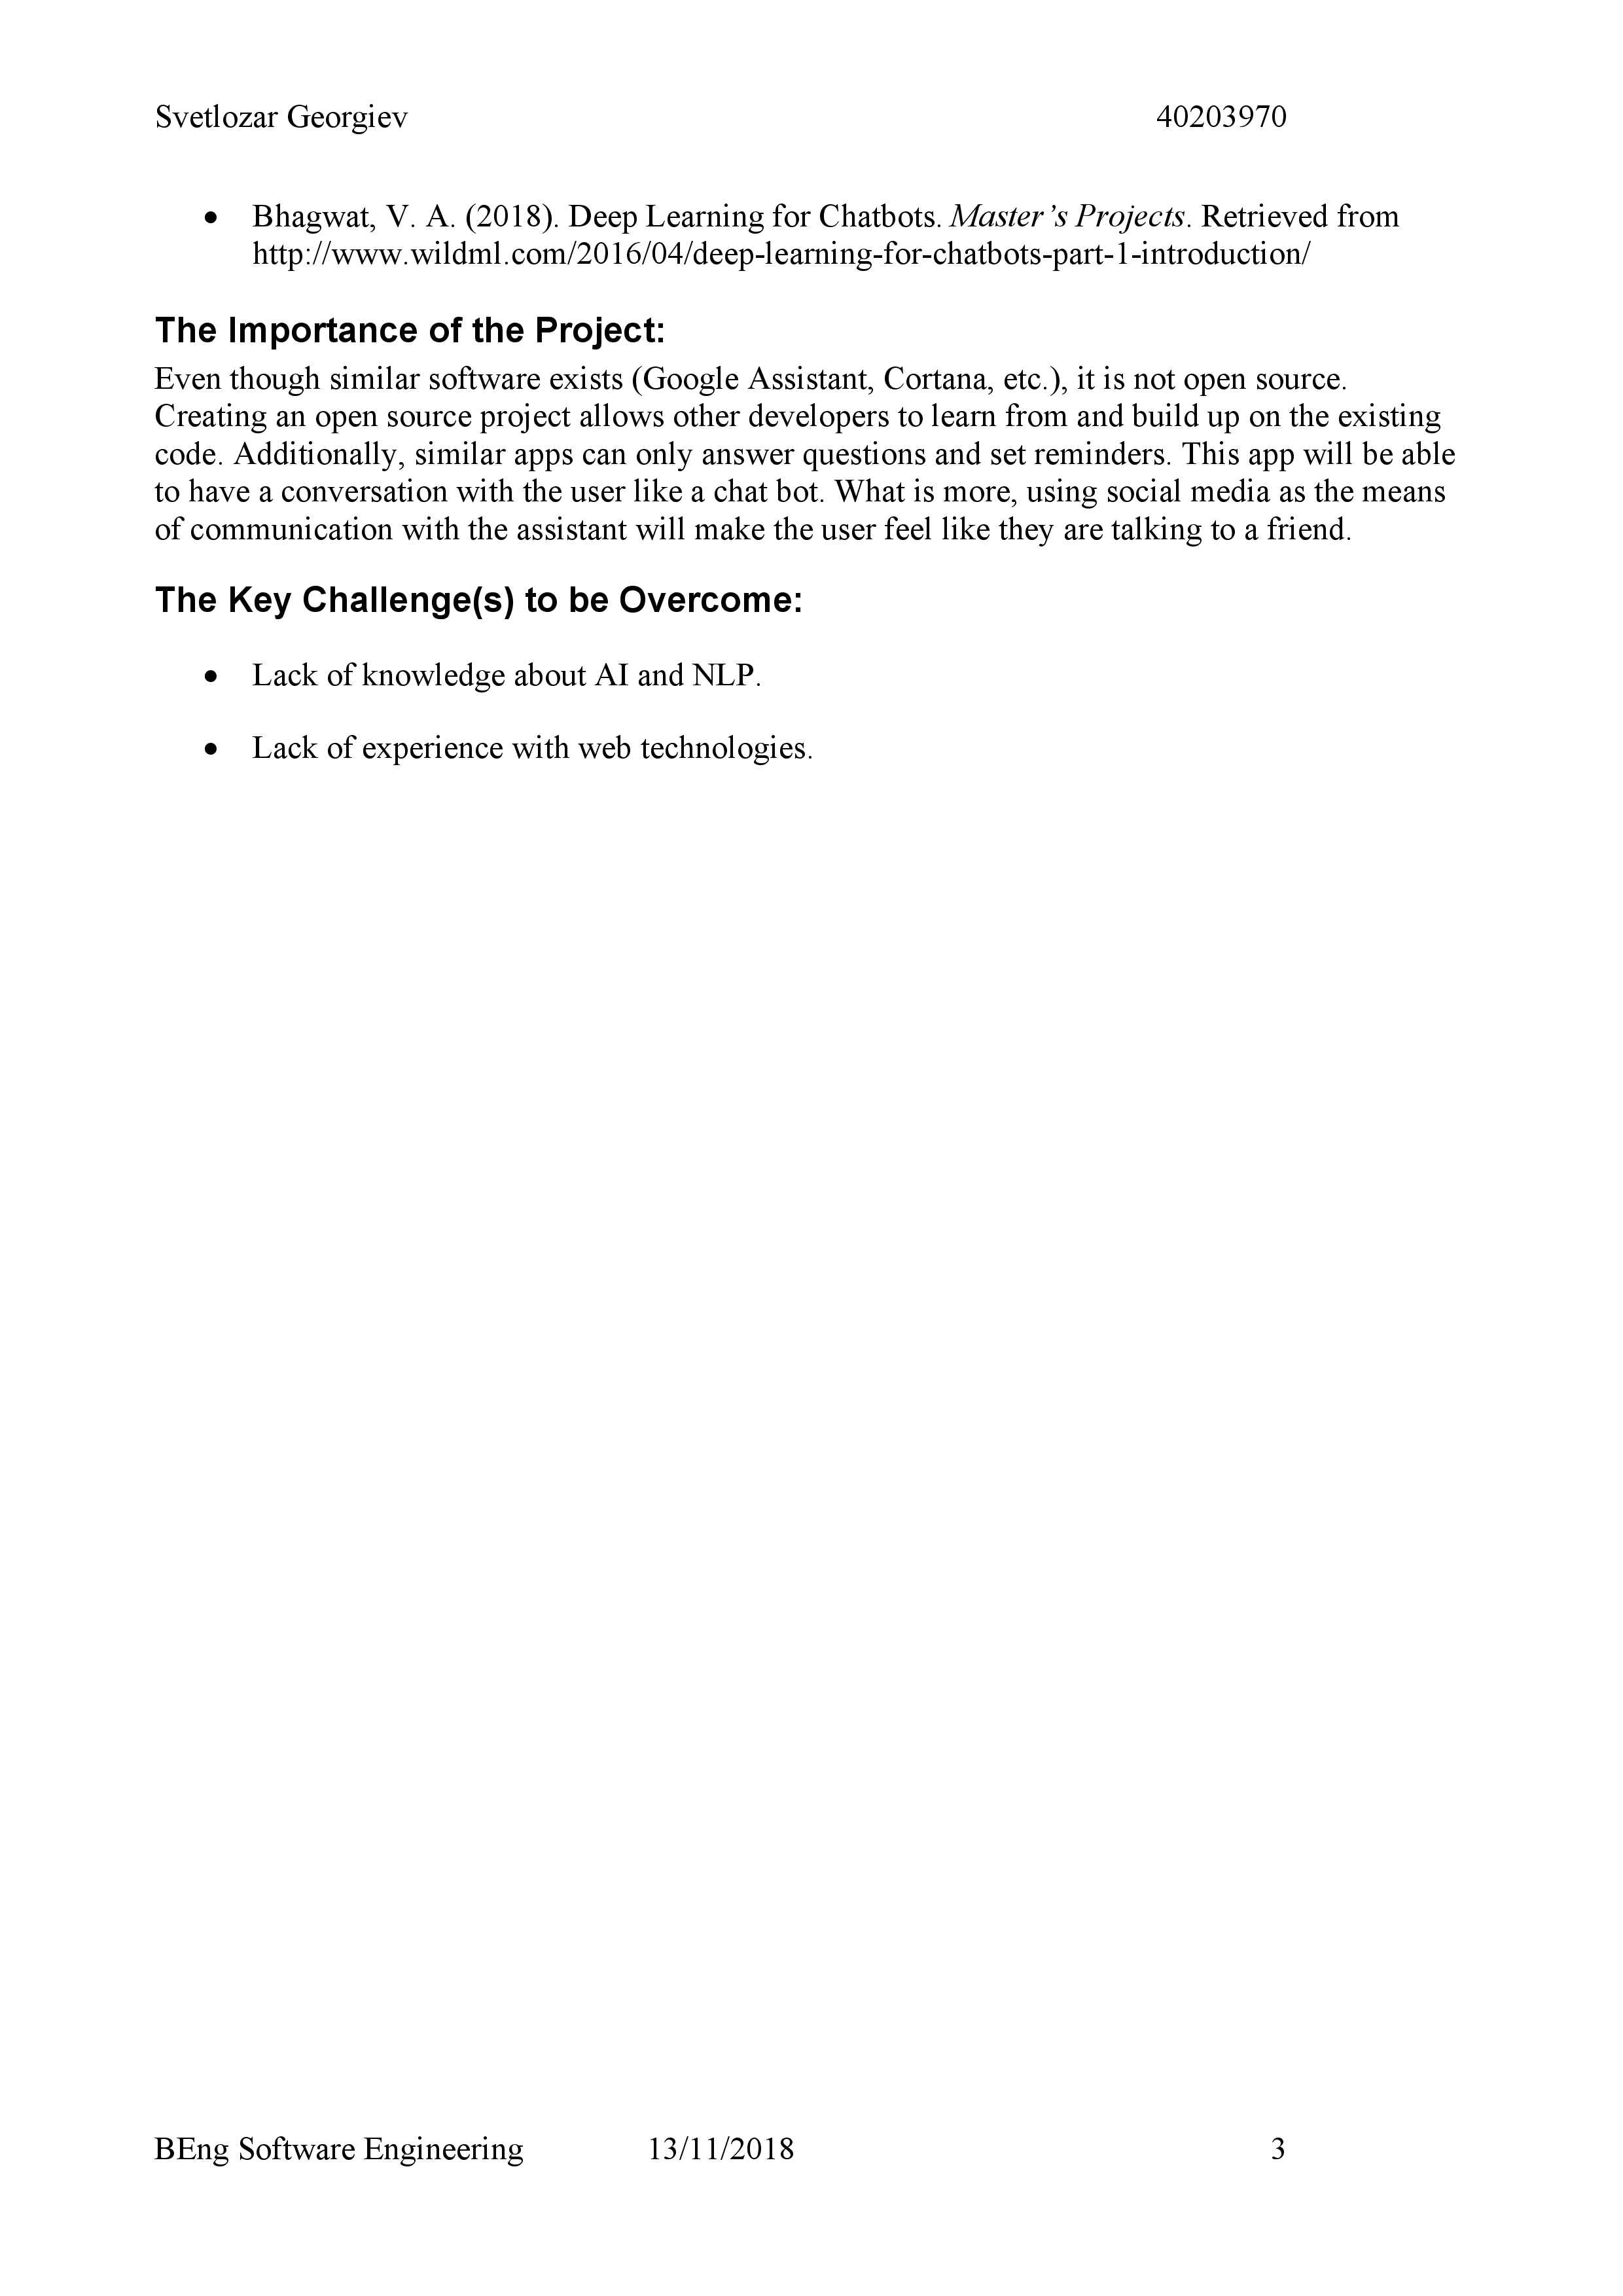
\includegraphics[width=\textwidth,height=\textheight,keepaspectratio]{IPO-2.png}

\newpage
\section{Diary Sheets}
% first semester
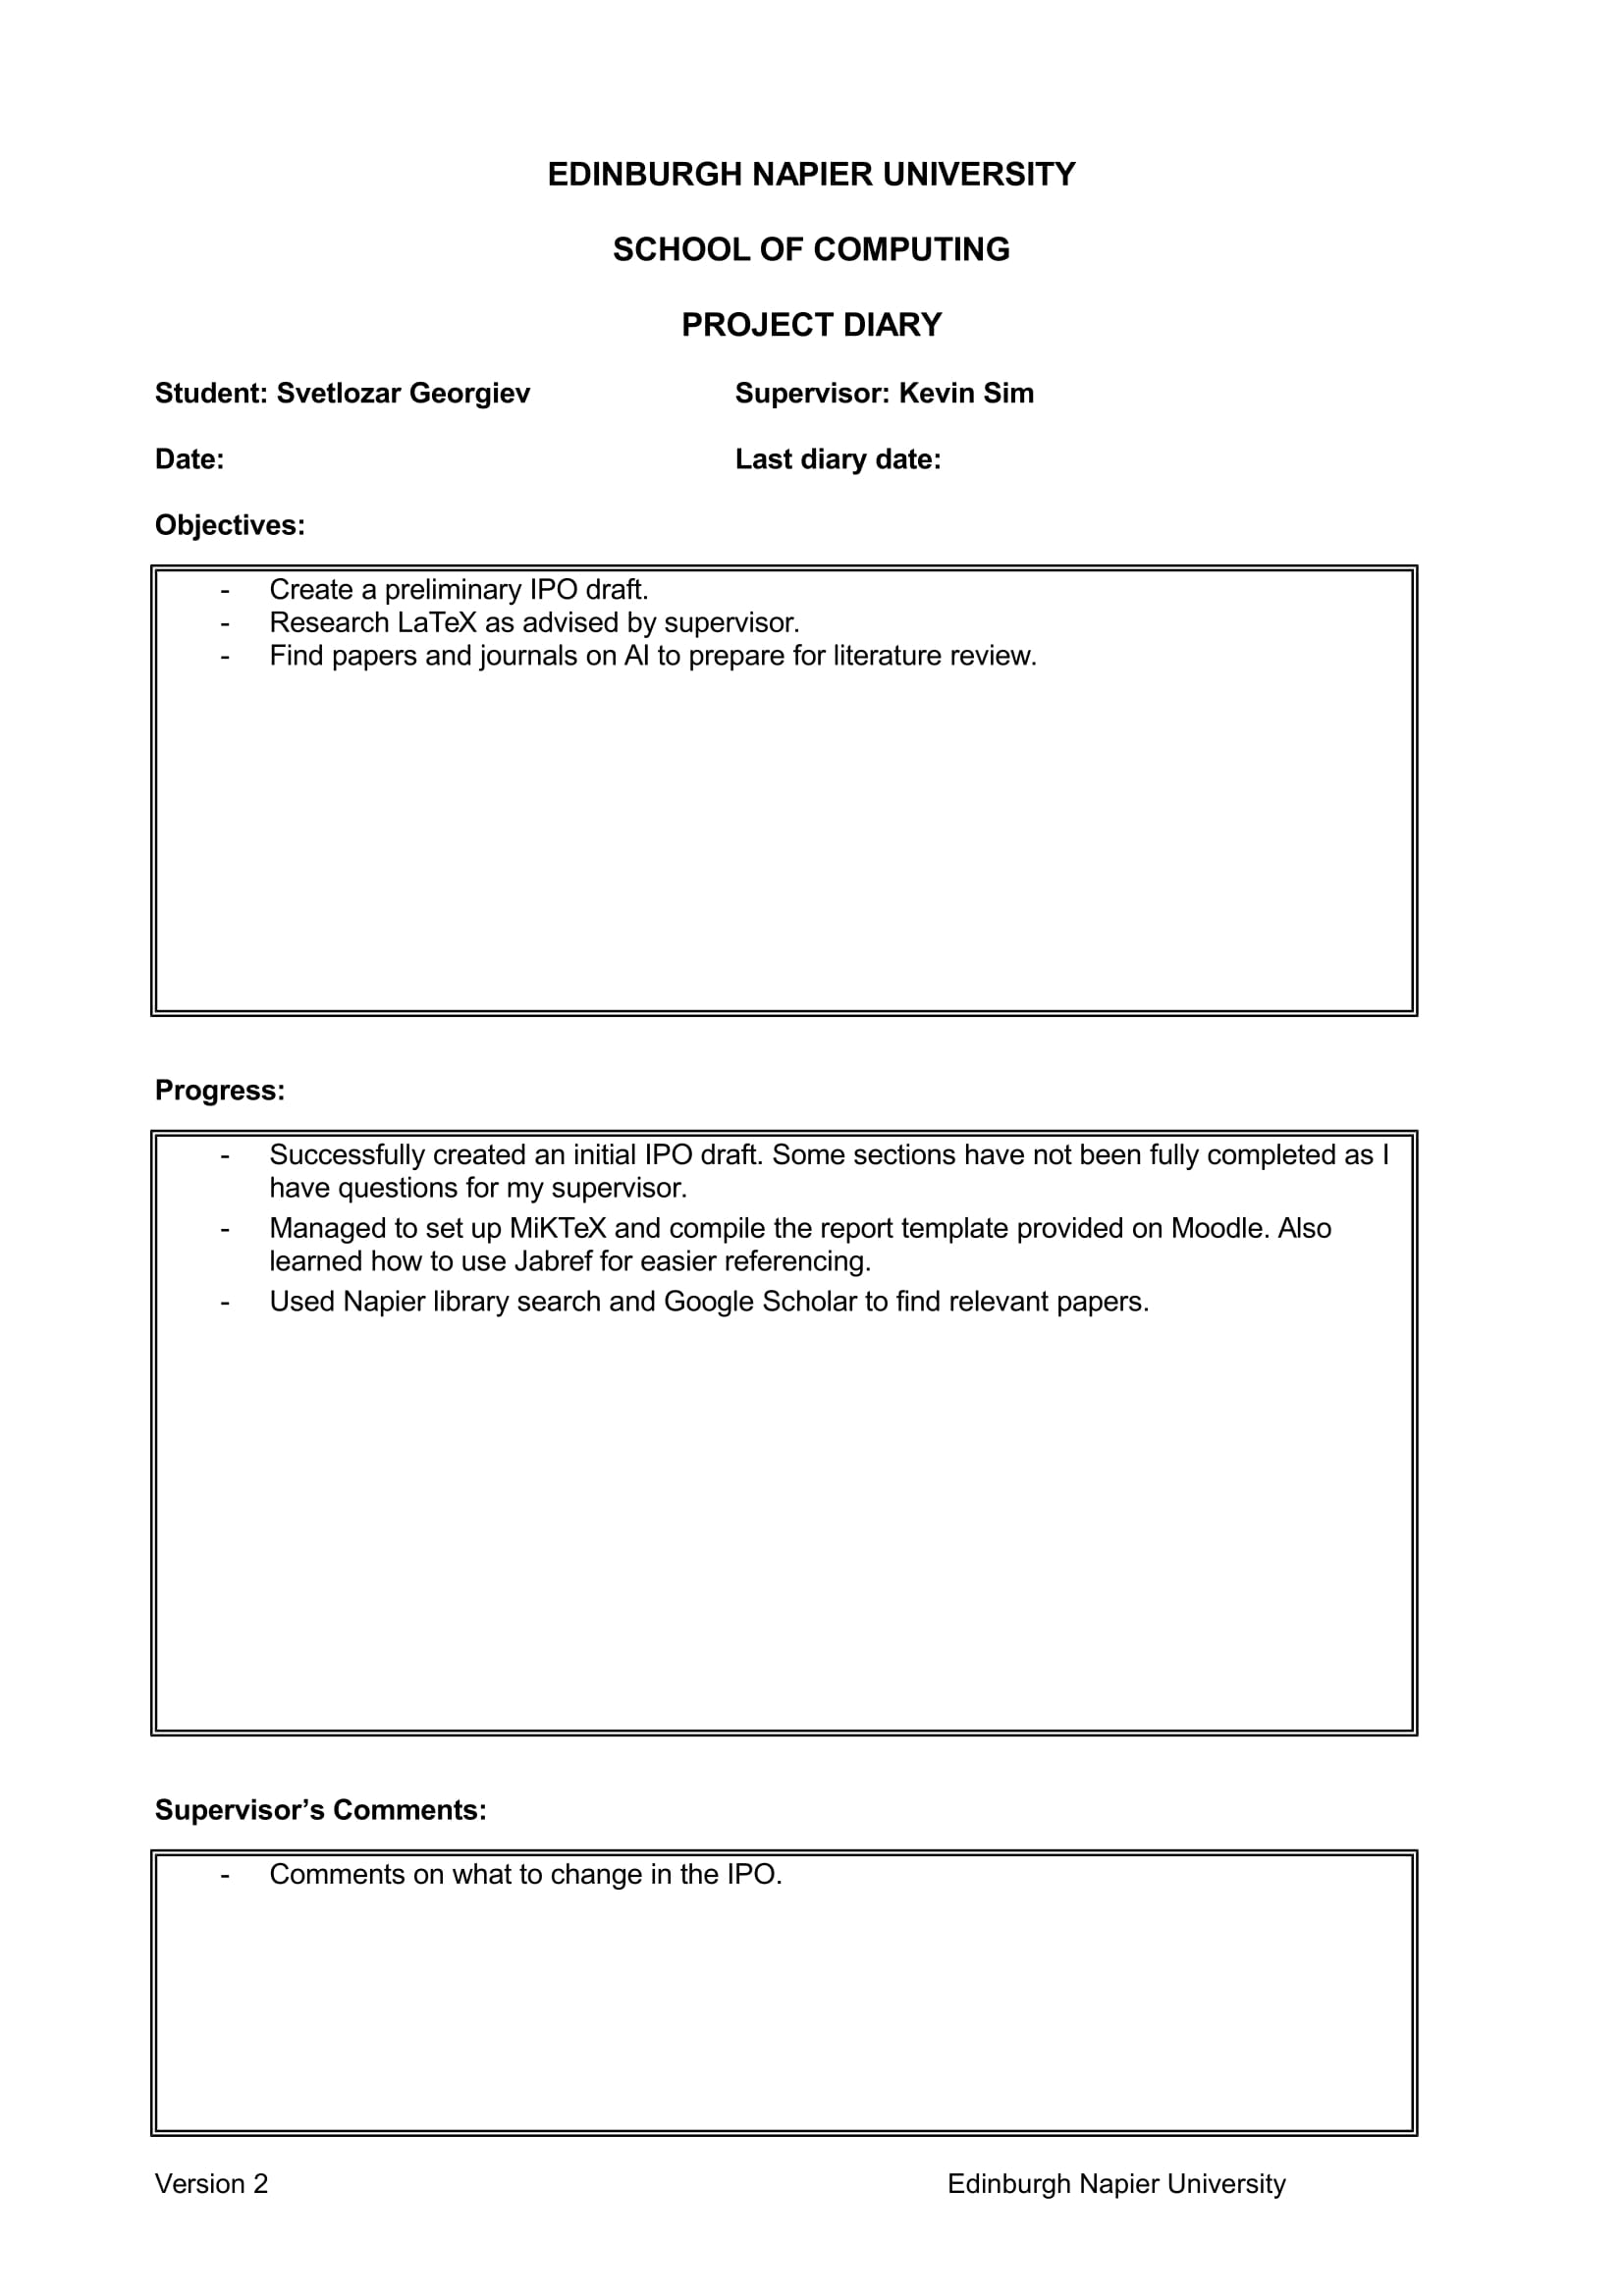
\includegraphics[width=\textwidth,height=\textheight,keepaspectratio]{week2.jpg} % fit images to page
\newpage
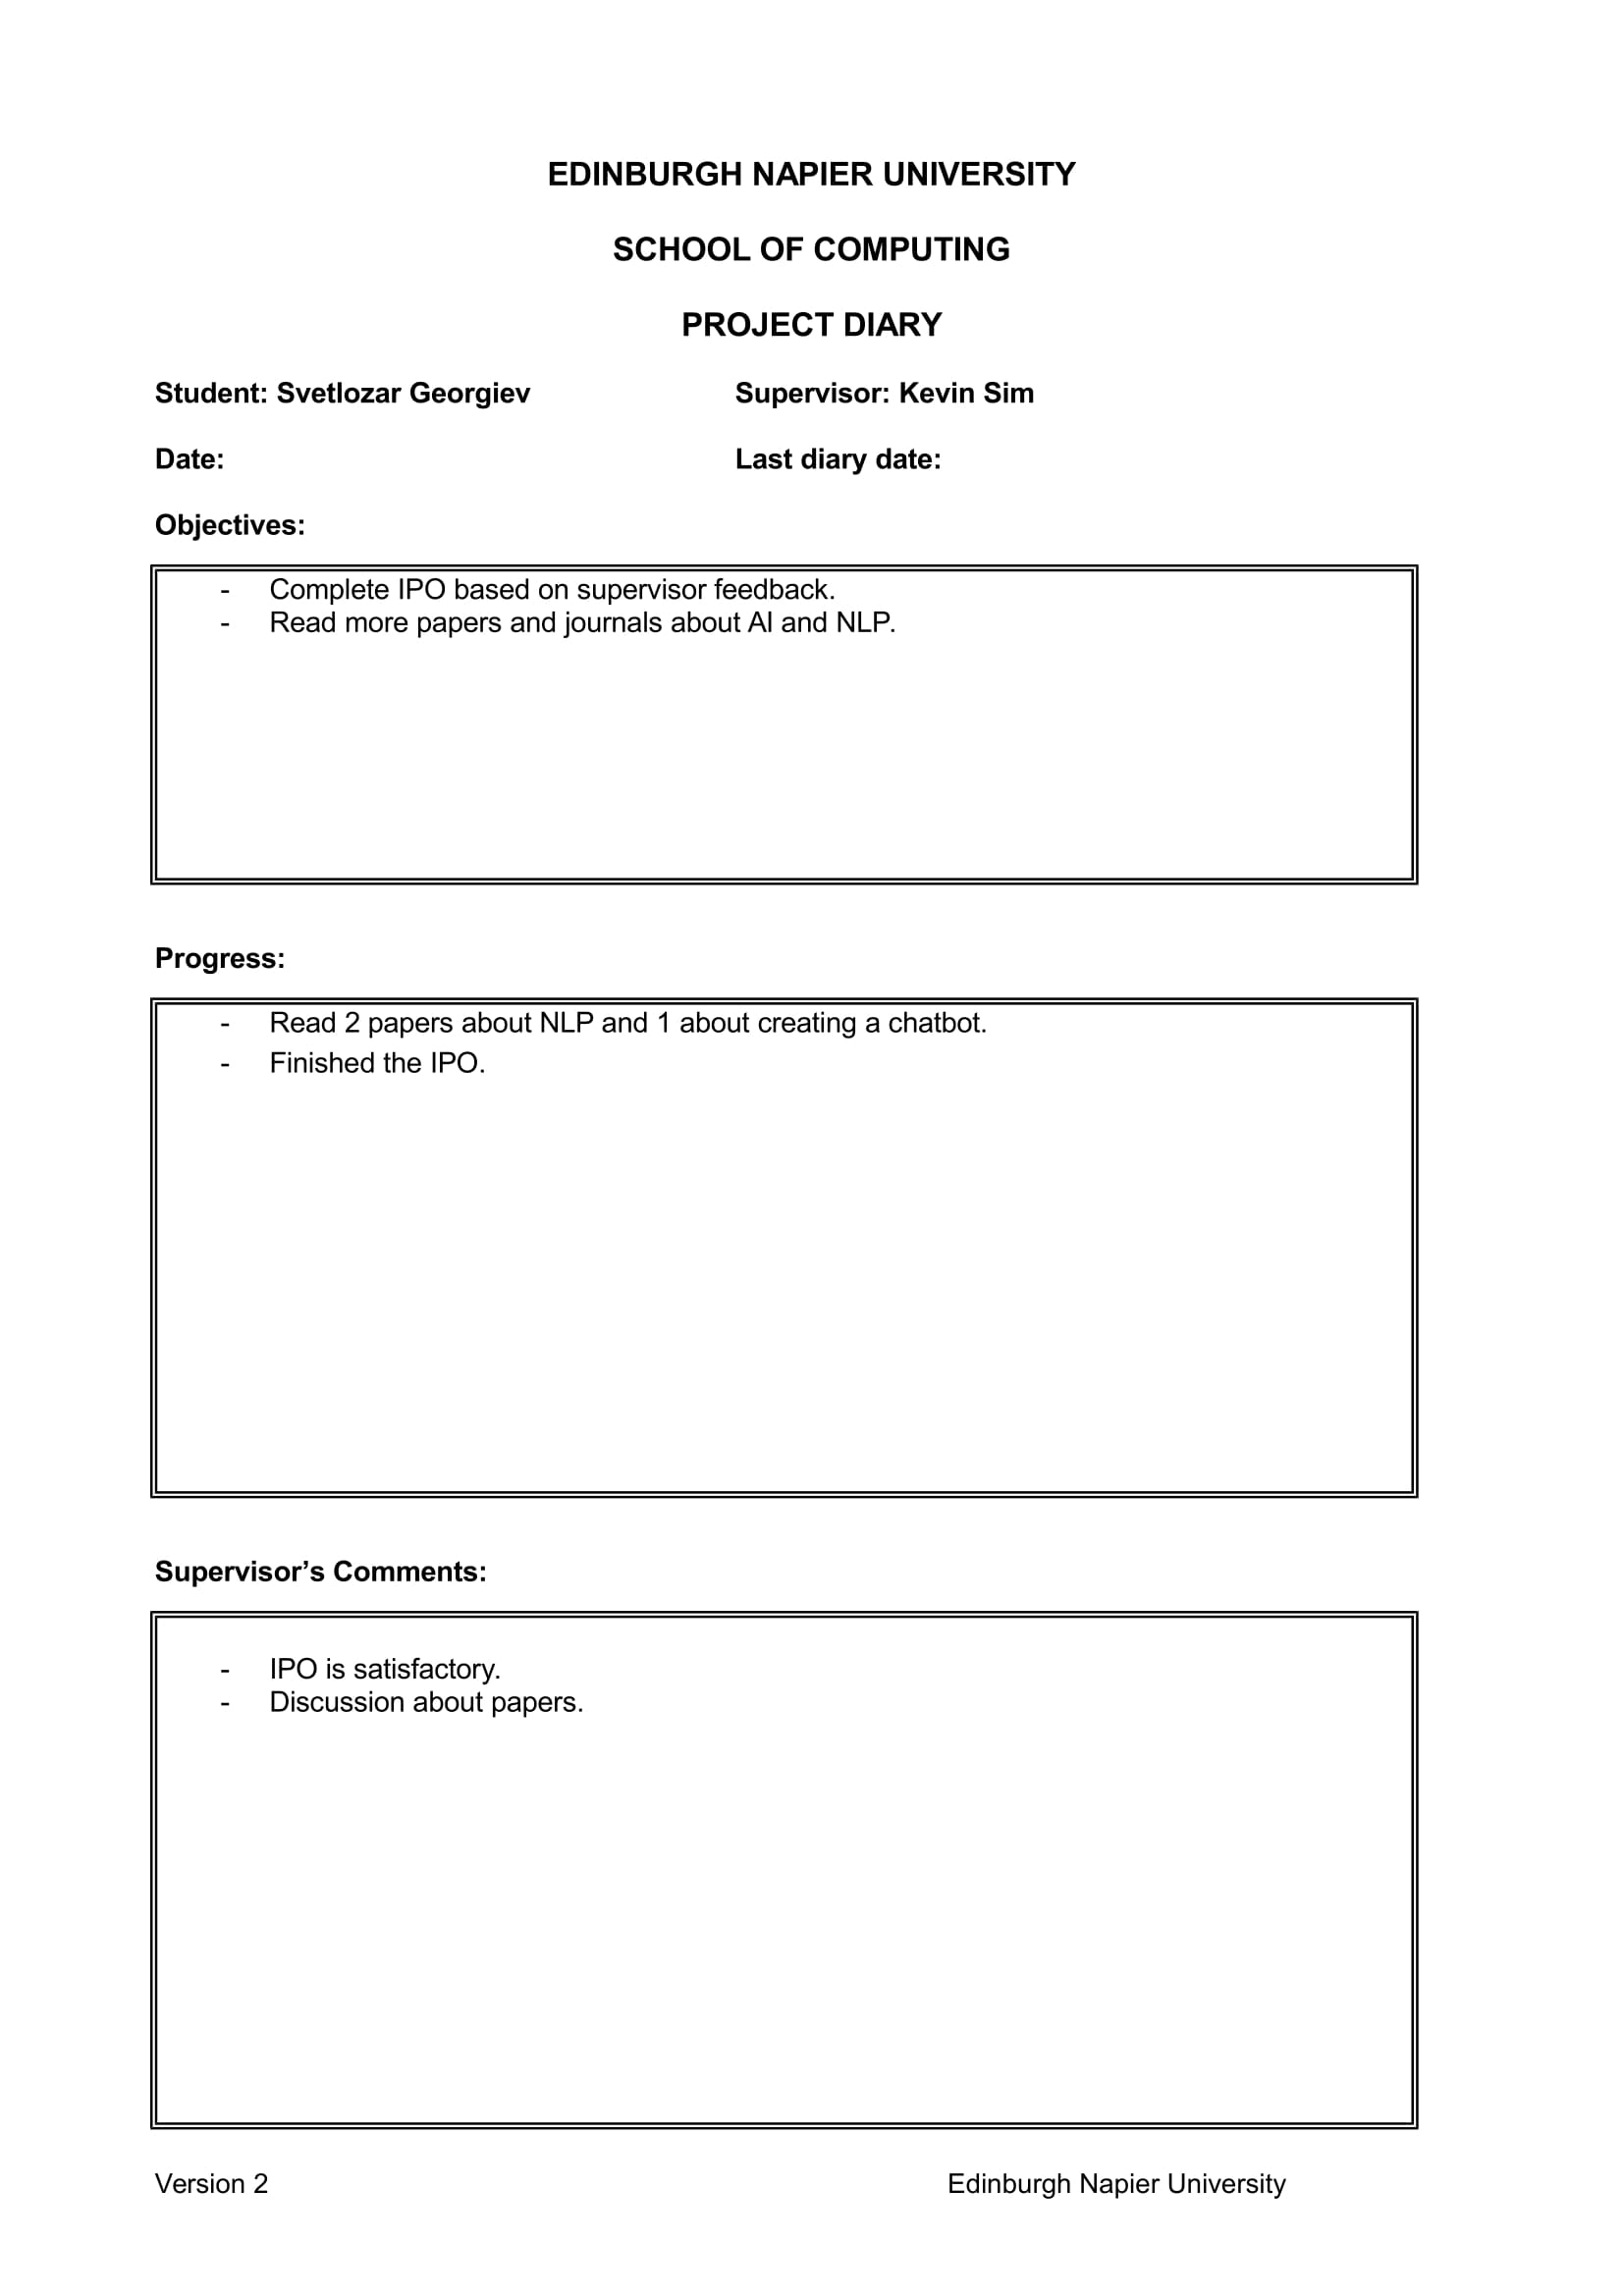
\includegraphics[width=\textwidth,height=\textheight,keepaspectratio]{week3.jpg}
\newpage
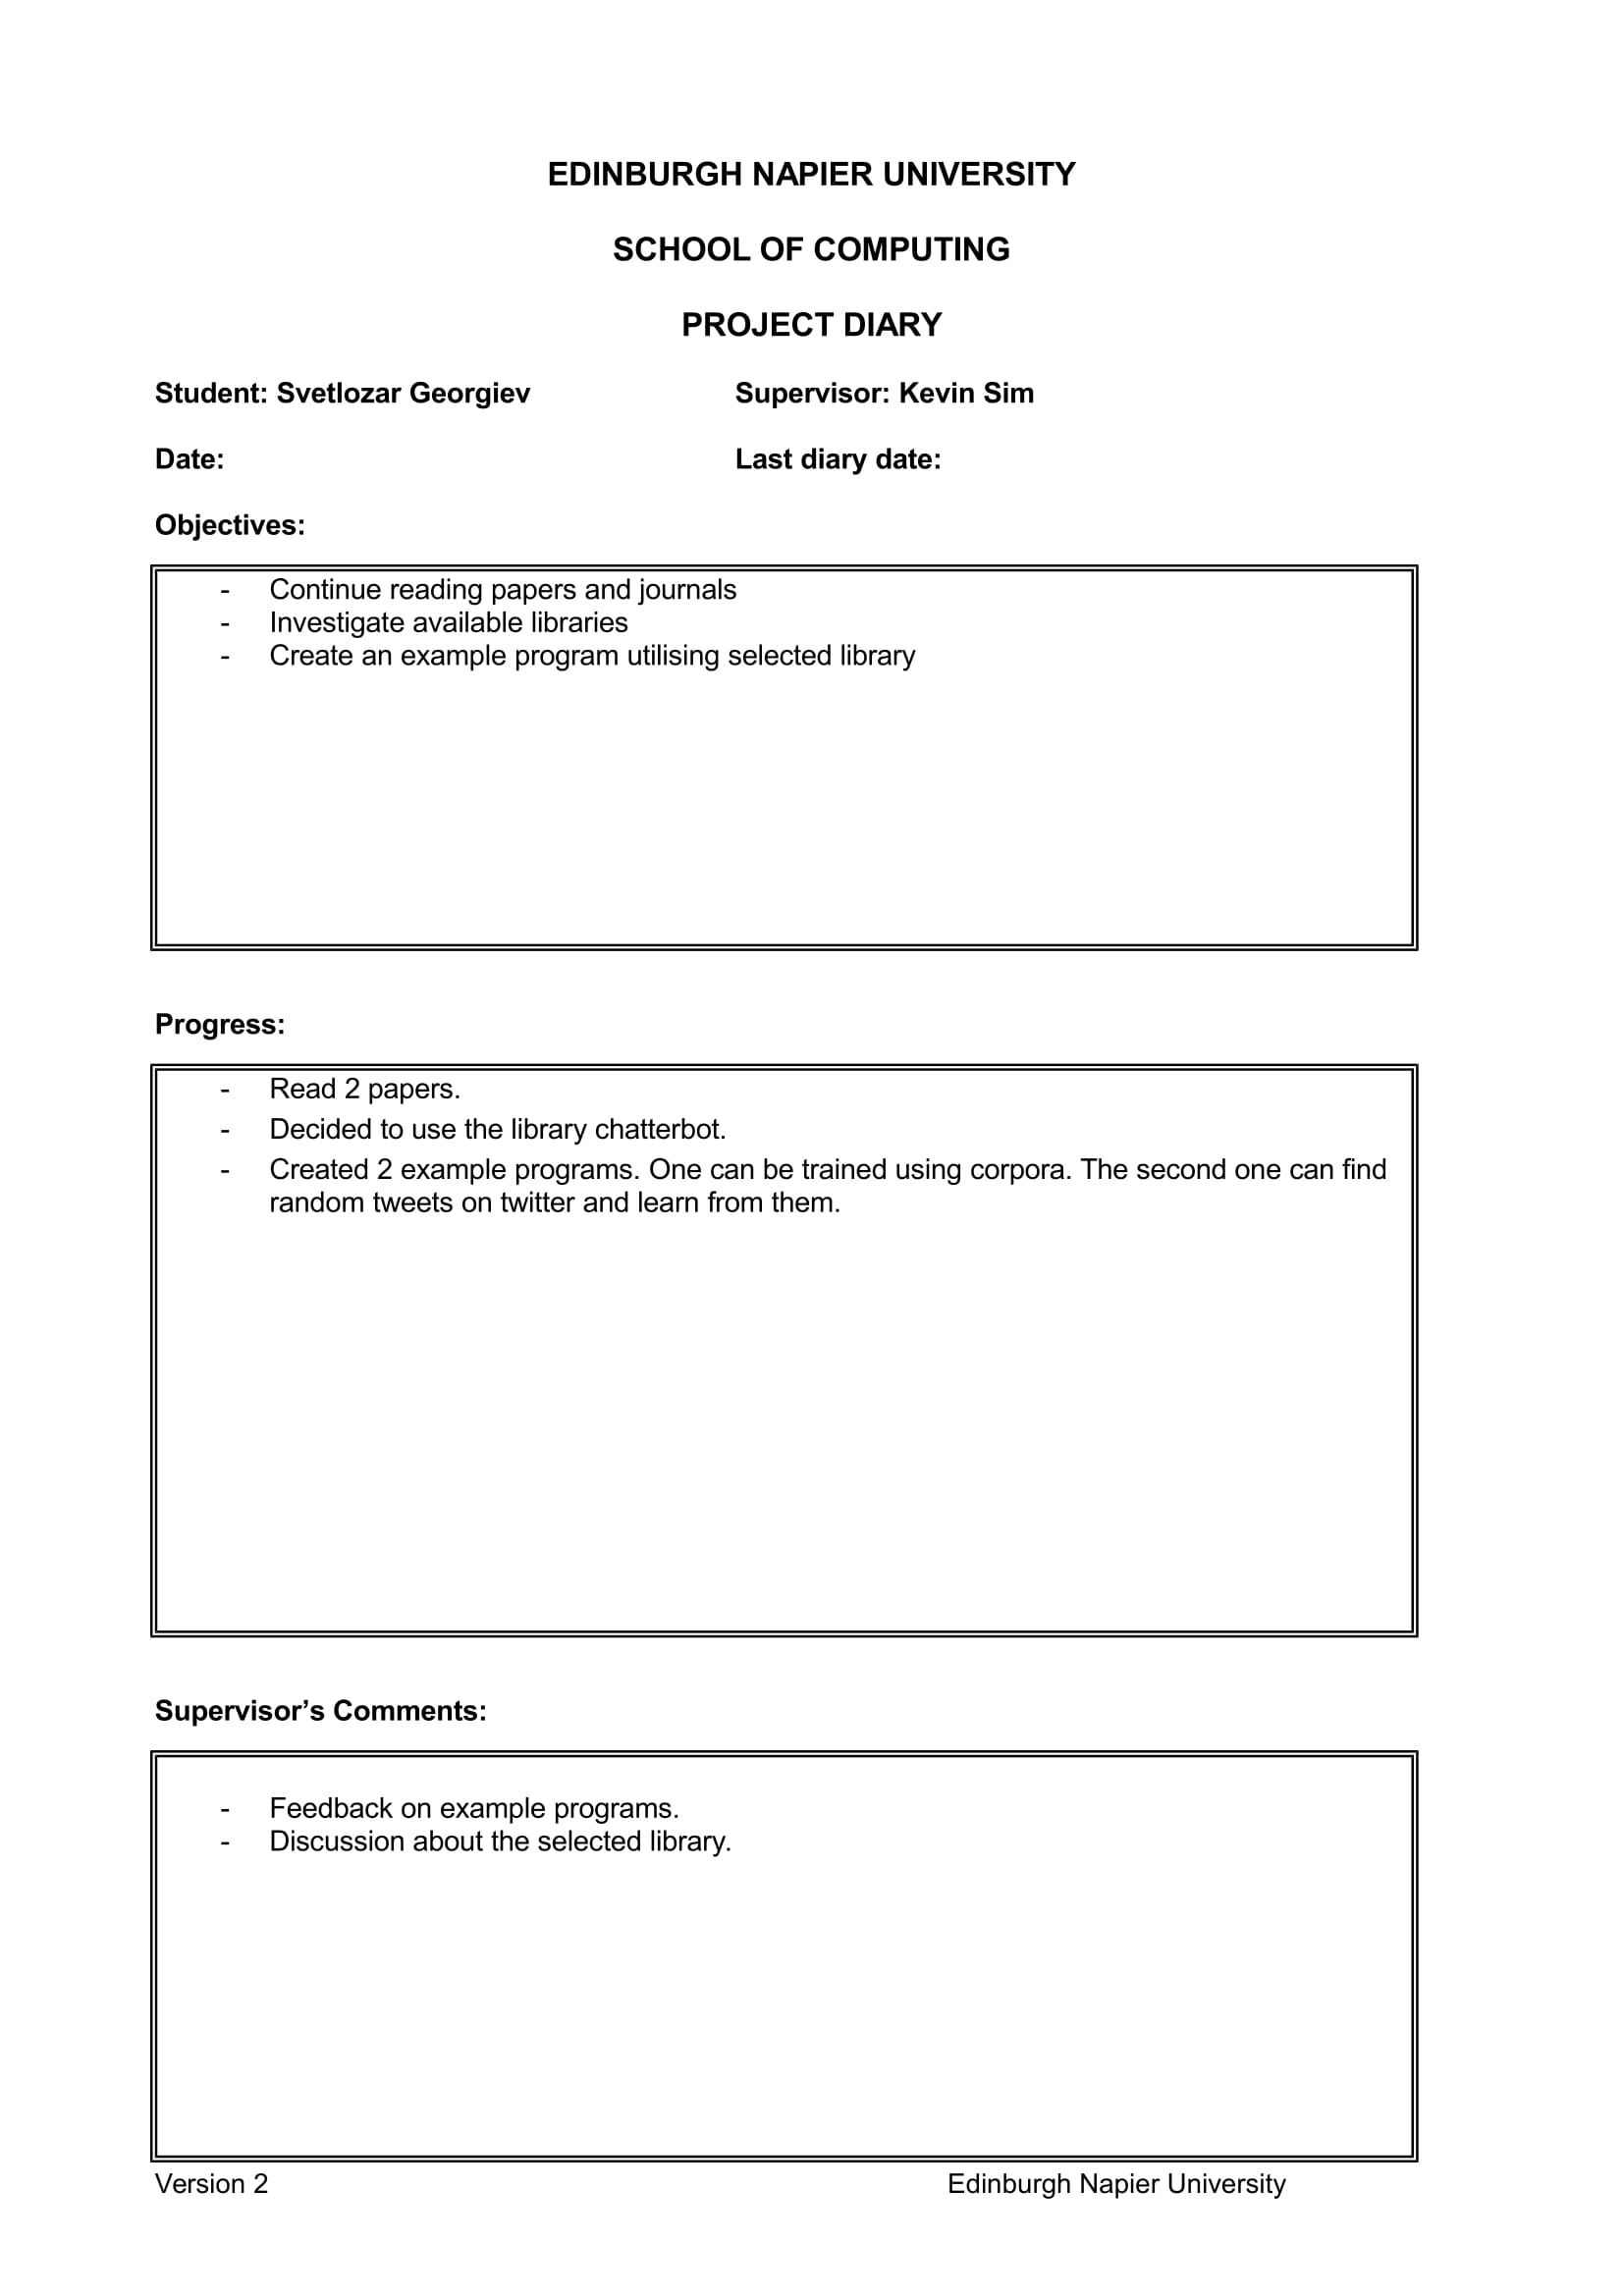
\includegraphics[width=\textwidth,height=\textheight,keepaspectratio]{week4.jpg}
\newpage
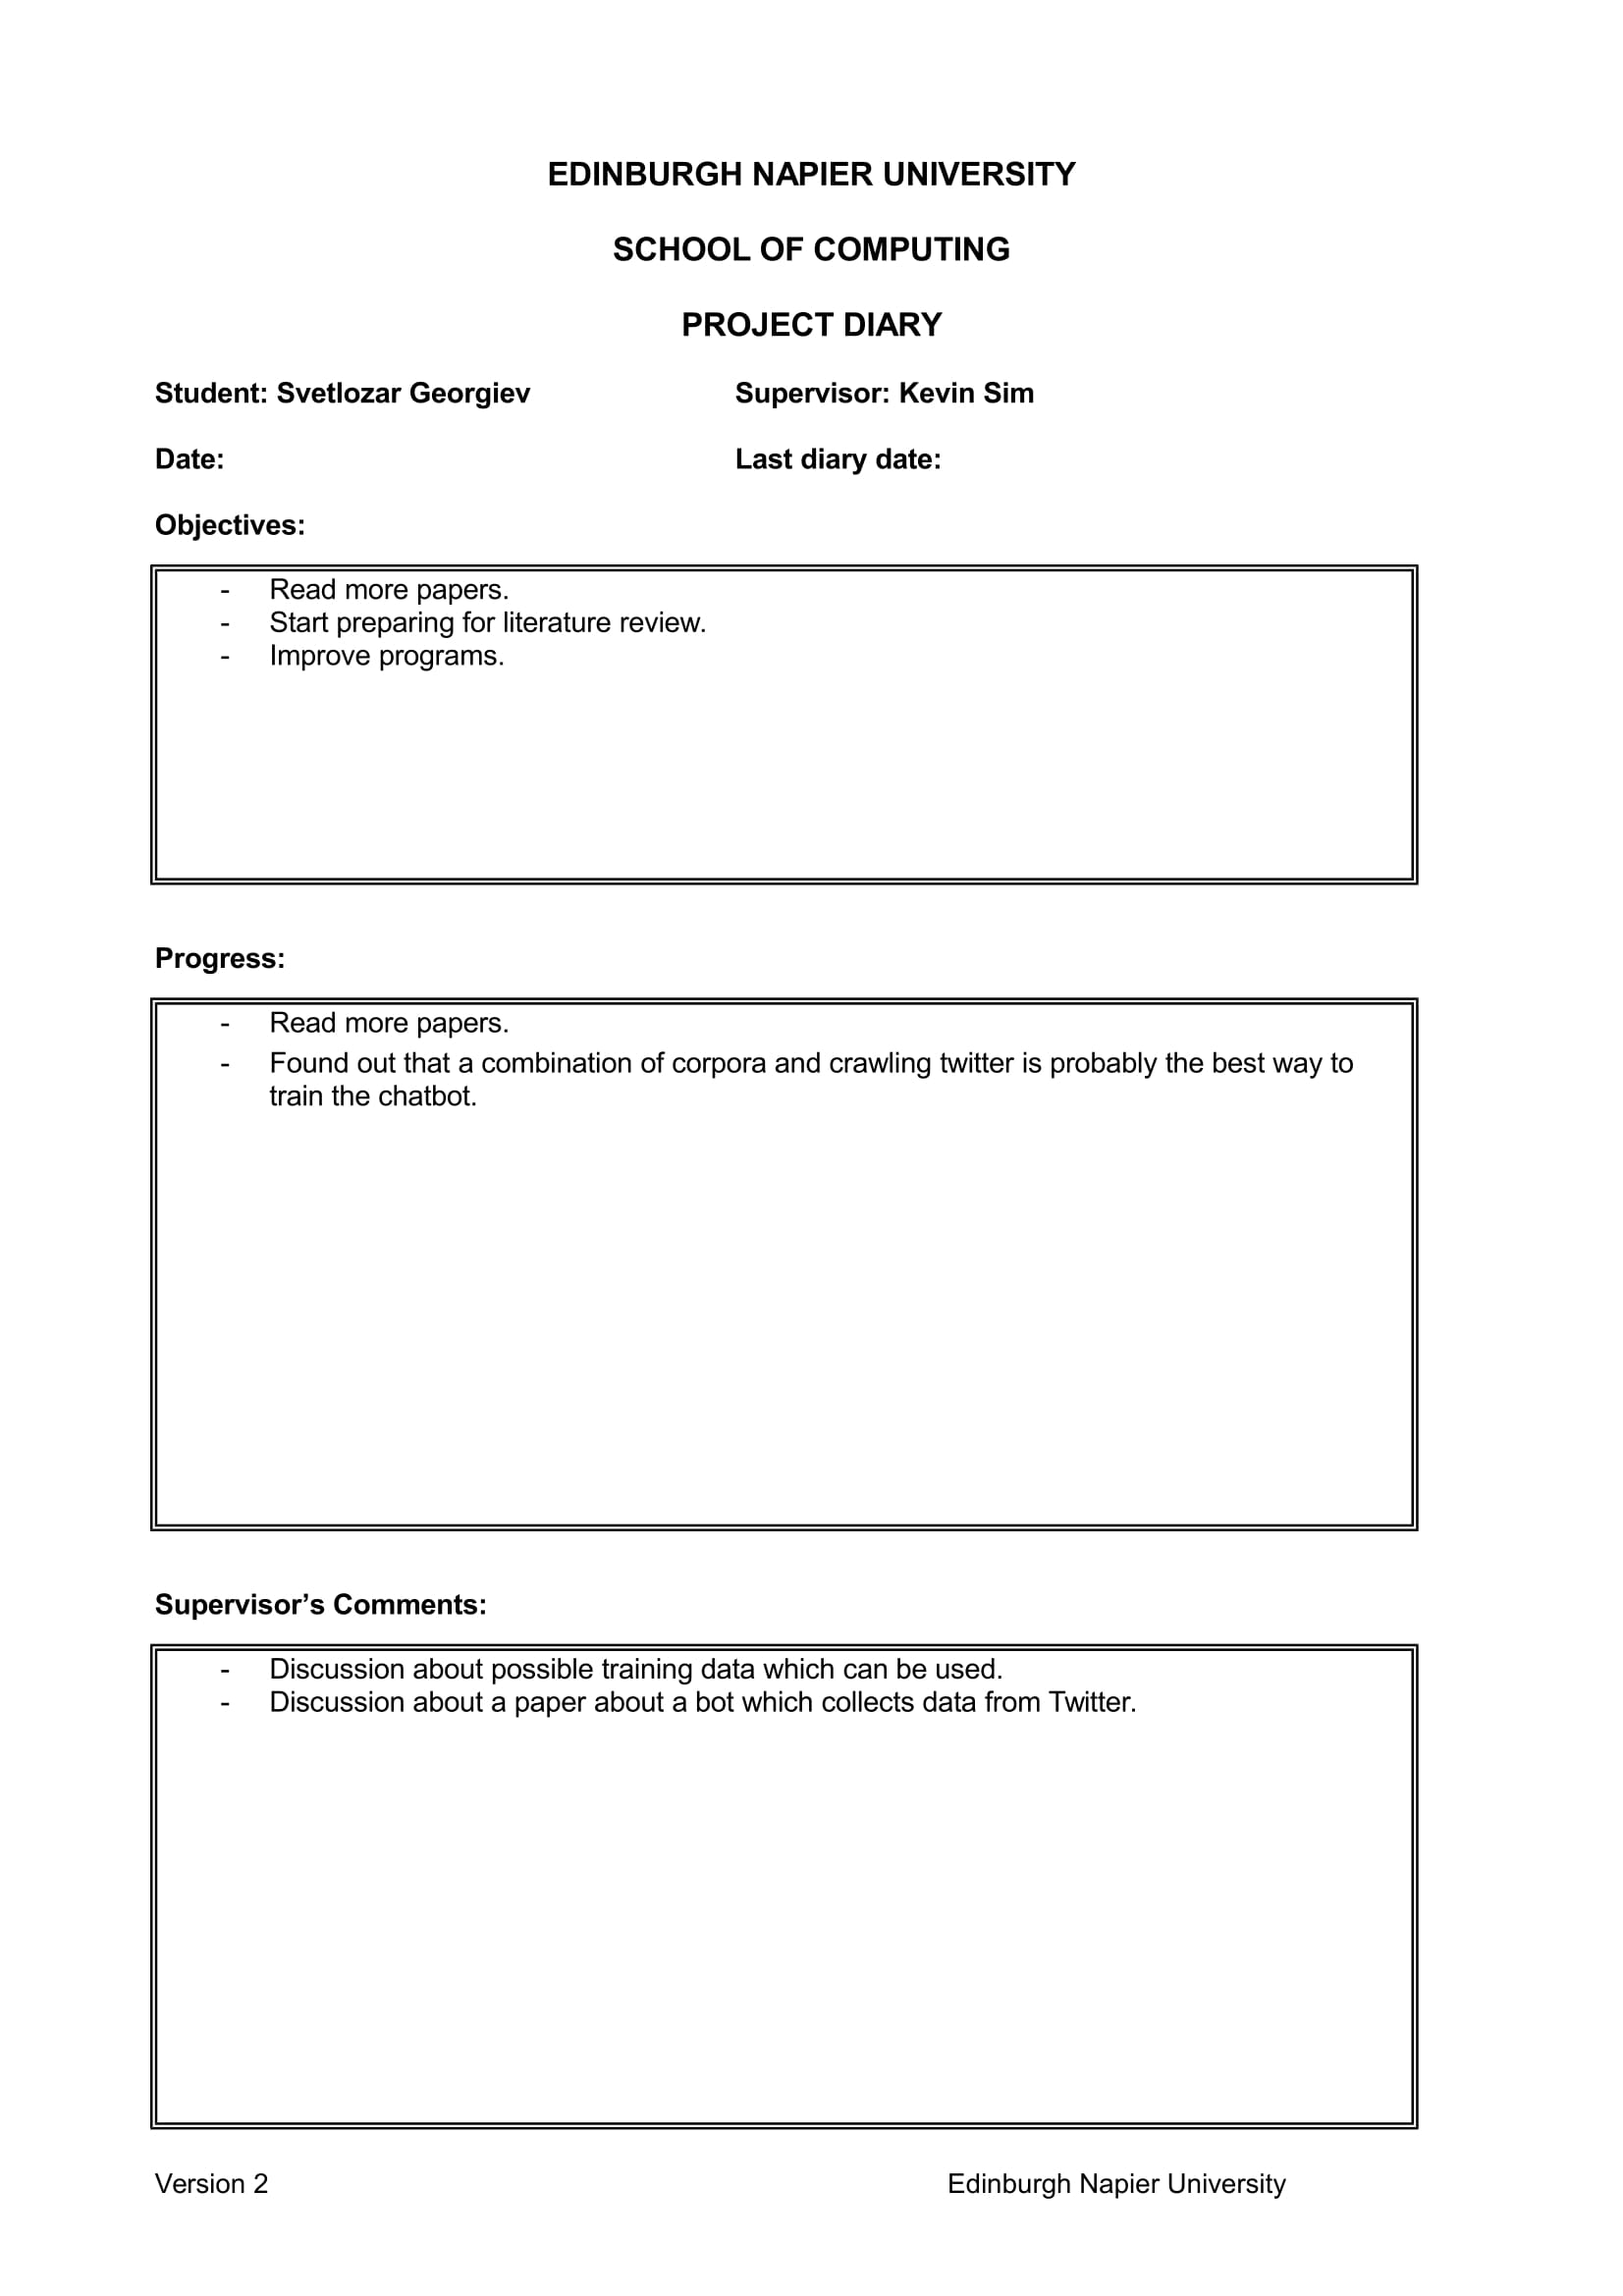
\includegraphics[width=\textwidth,height=\textheight,keepaspectratio]{week5.jpg}
\newpage
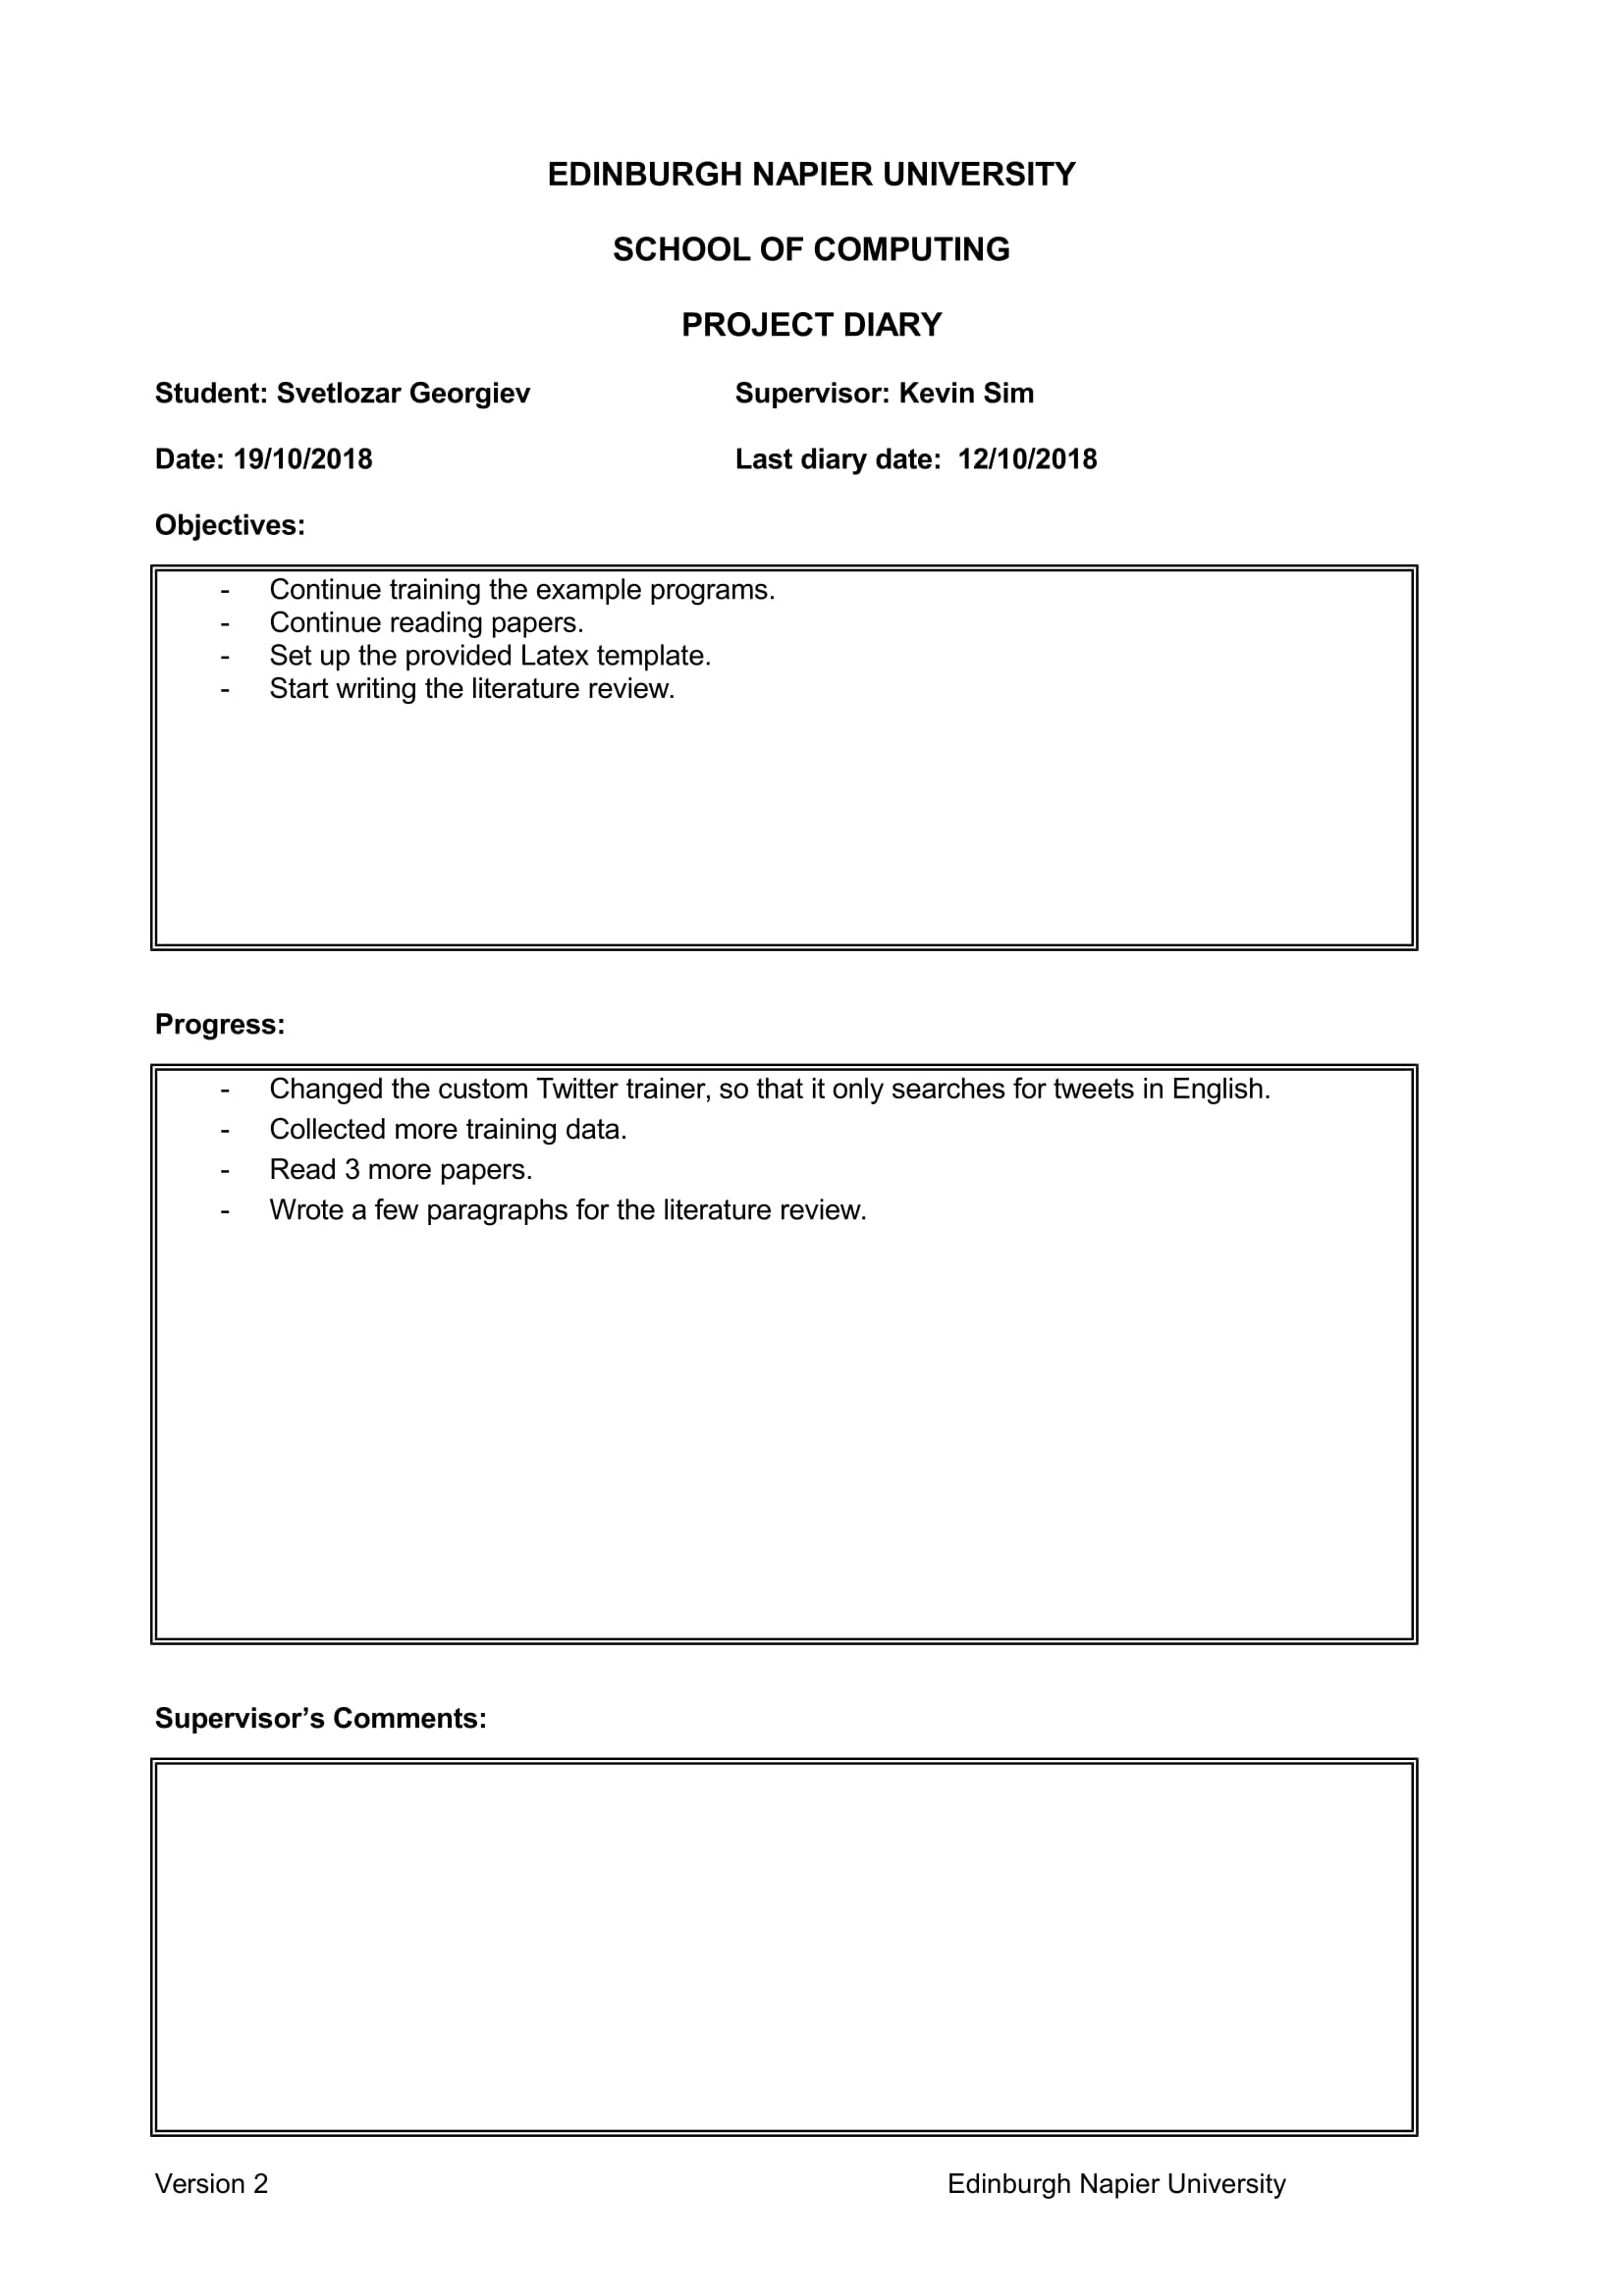
\includegraphics[width=\textwidth,height=\textheight,keepaspectratio]{week6.jpg}
\newpage
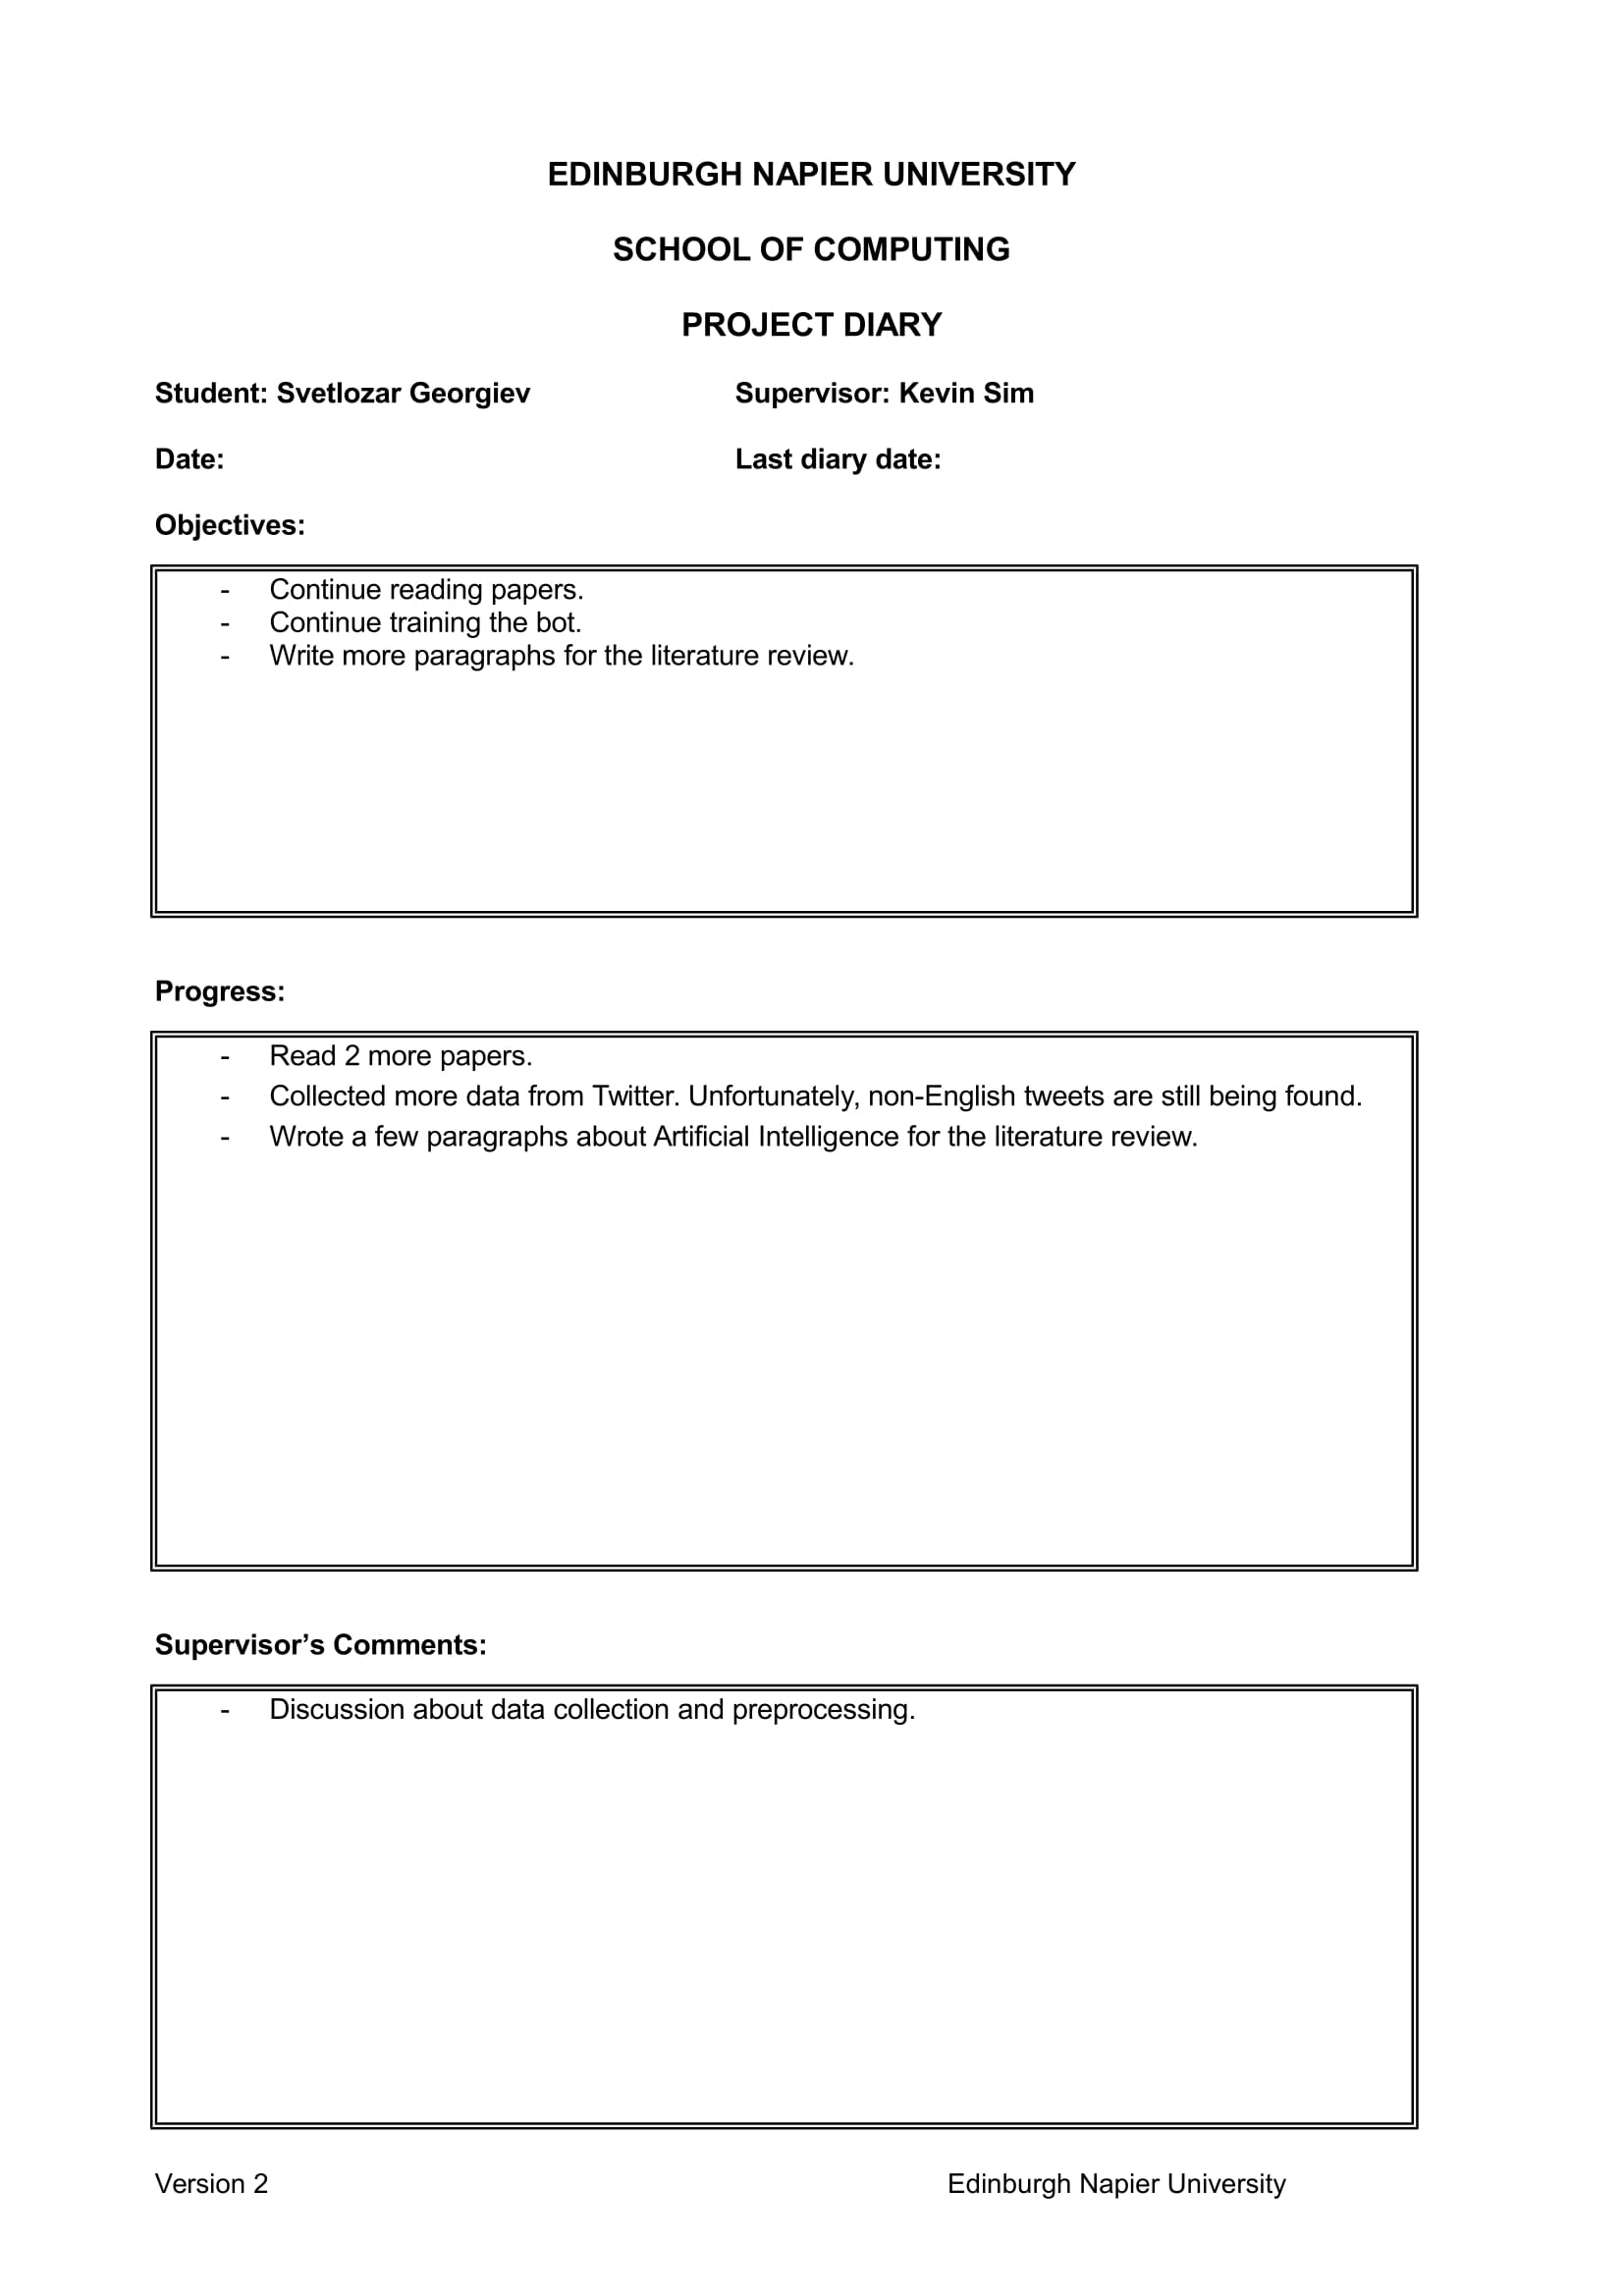
\includegraphics[width=\textwidth,height=\textheight,keepaspectratio]{week7.jpg}
\newpage
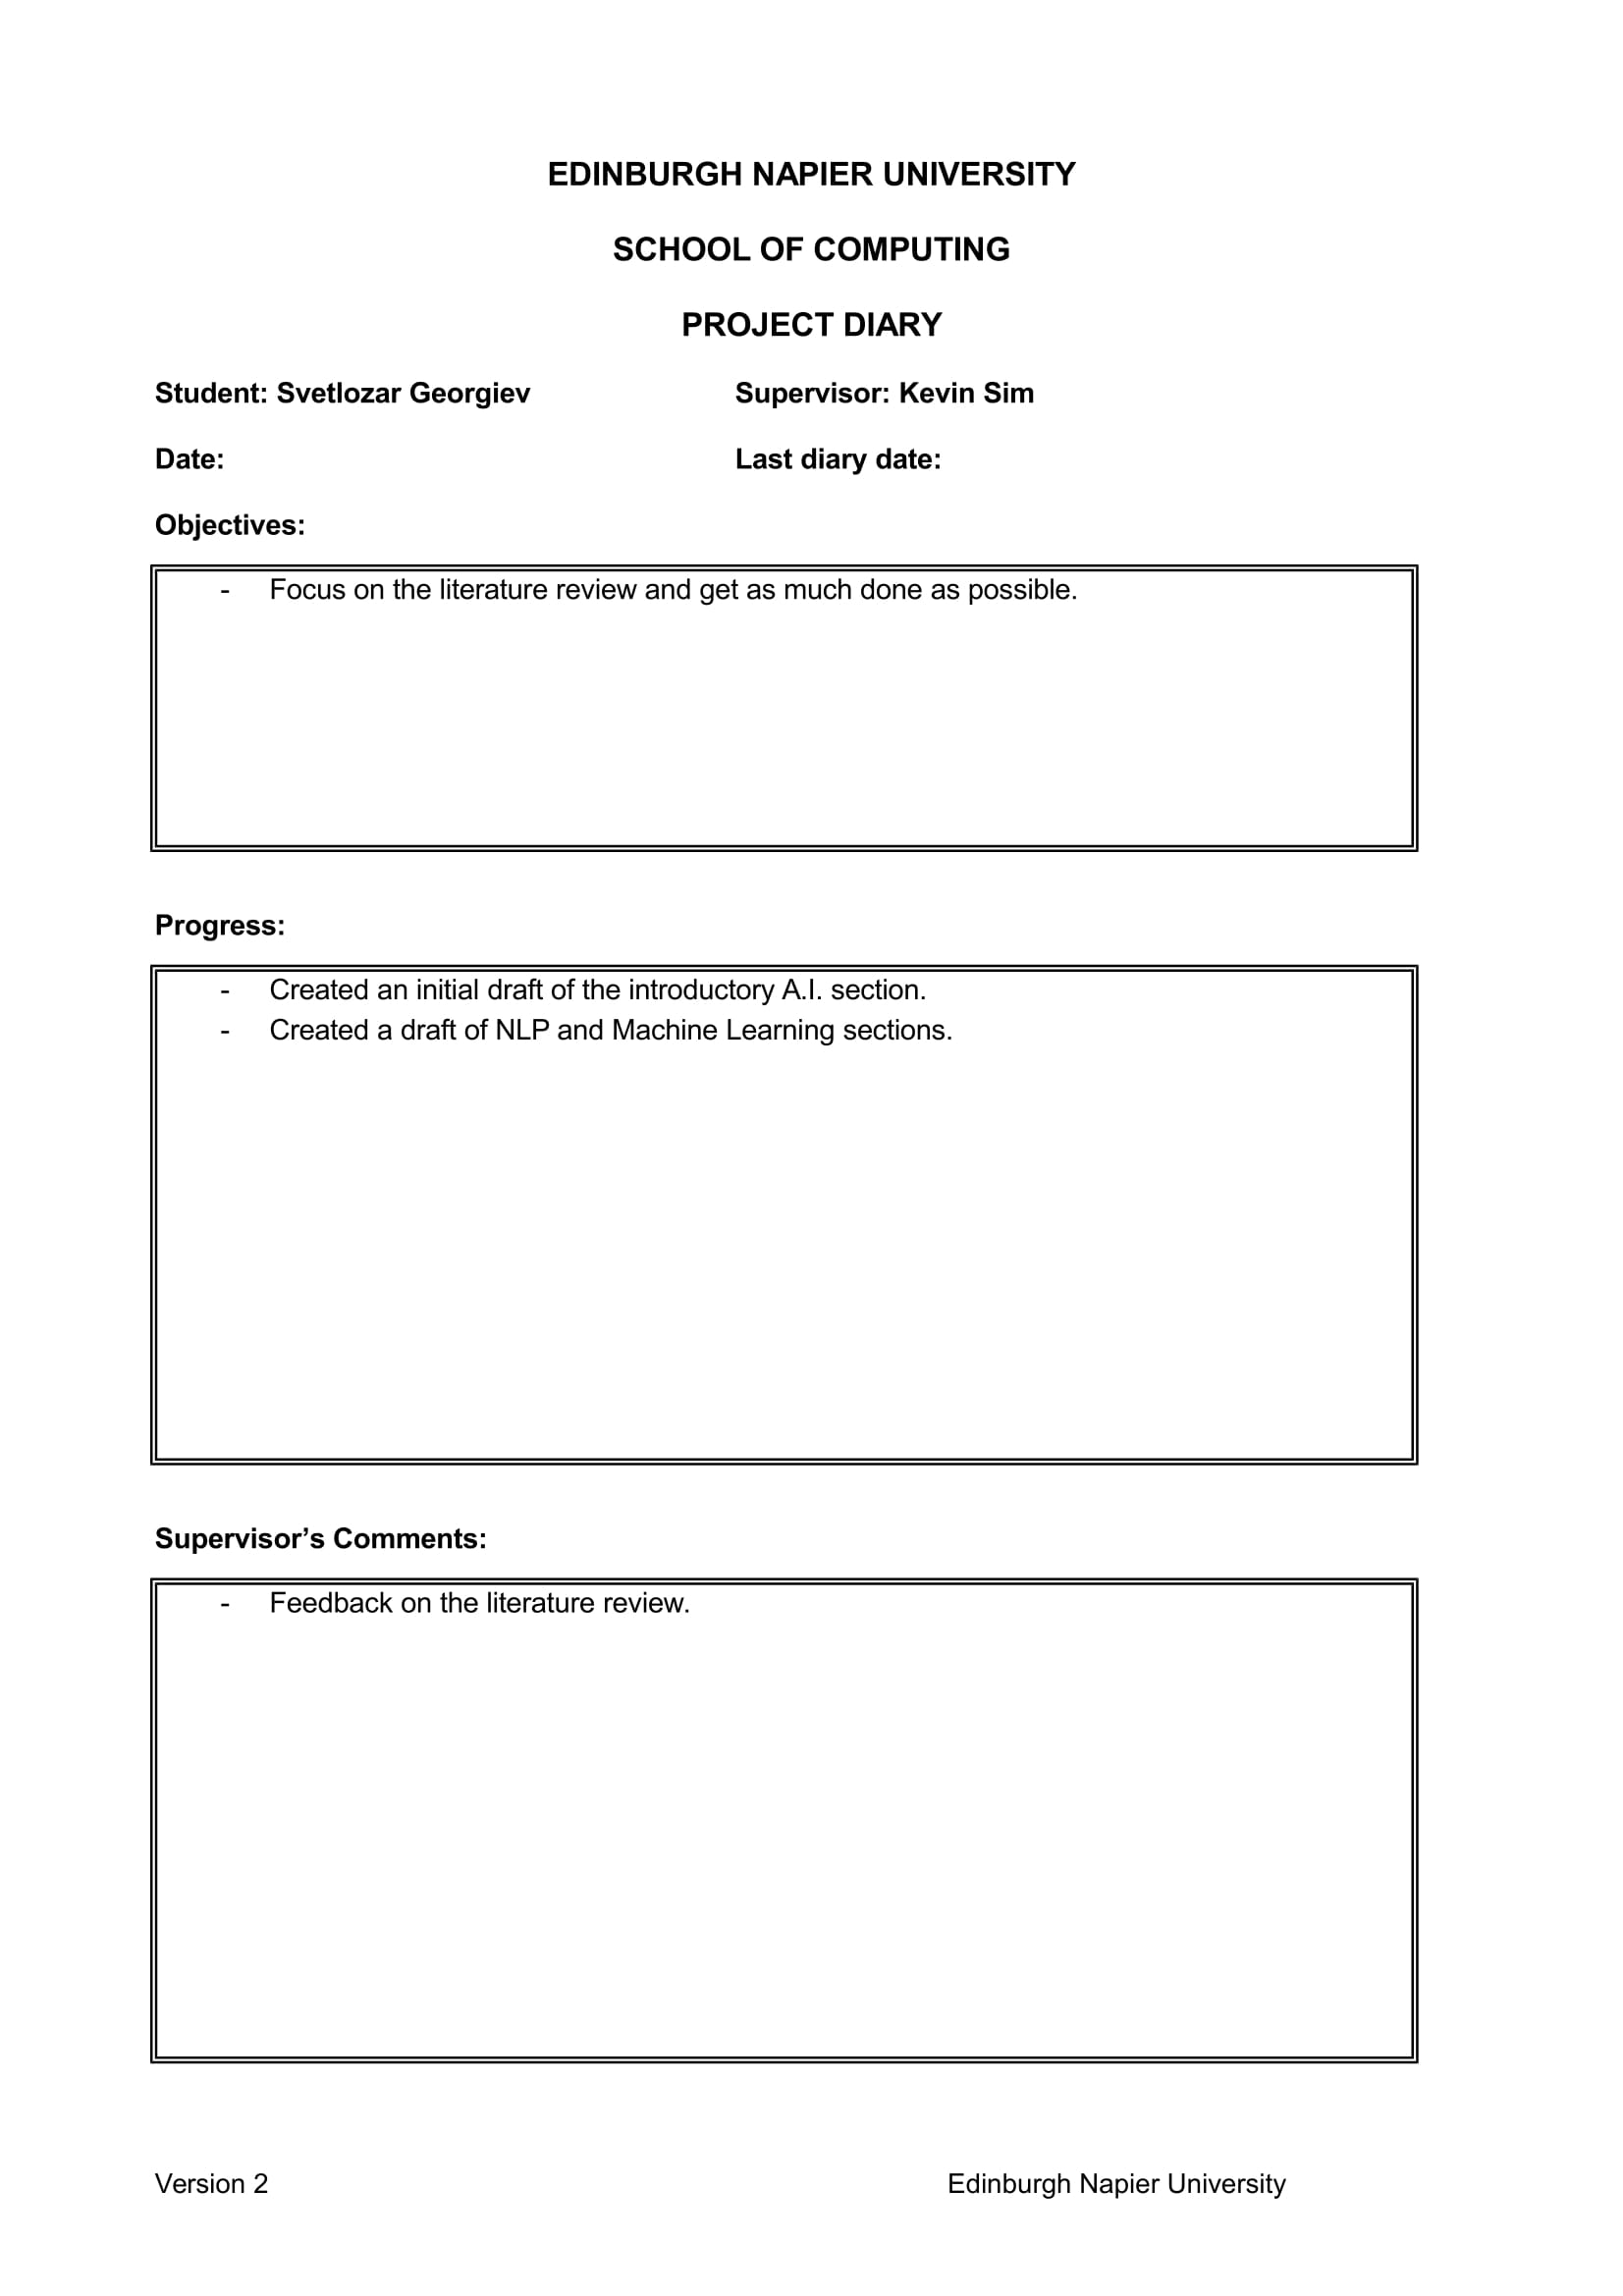
\includegraphics[width=\textwidth,height=\textheight,keepaspectratio]{week8.jpg}
\newpage
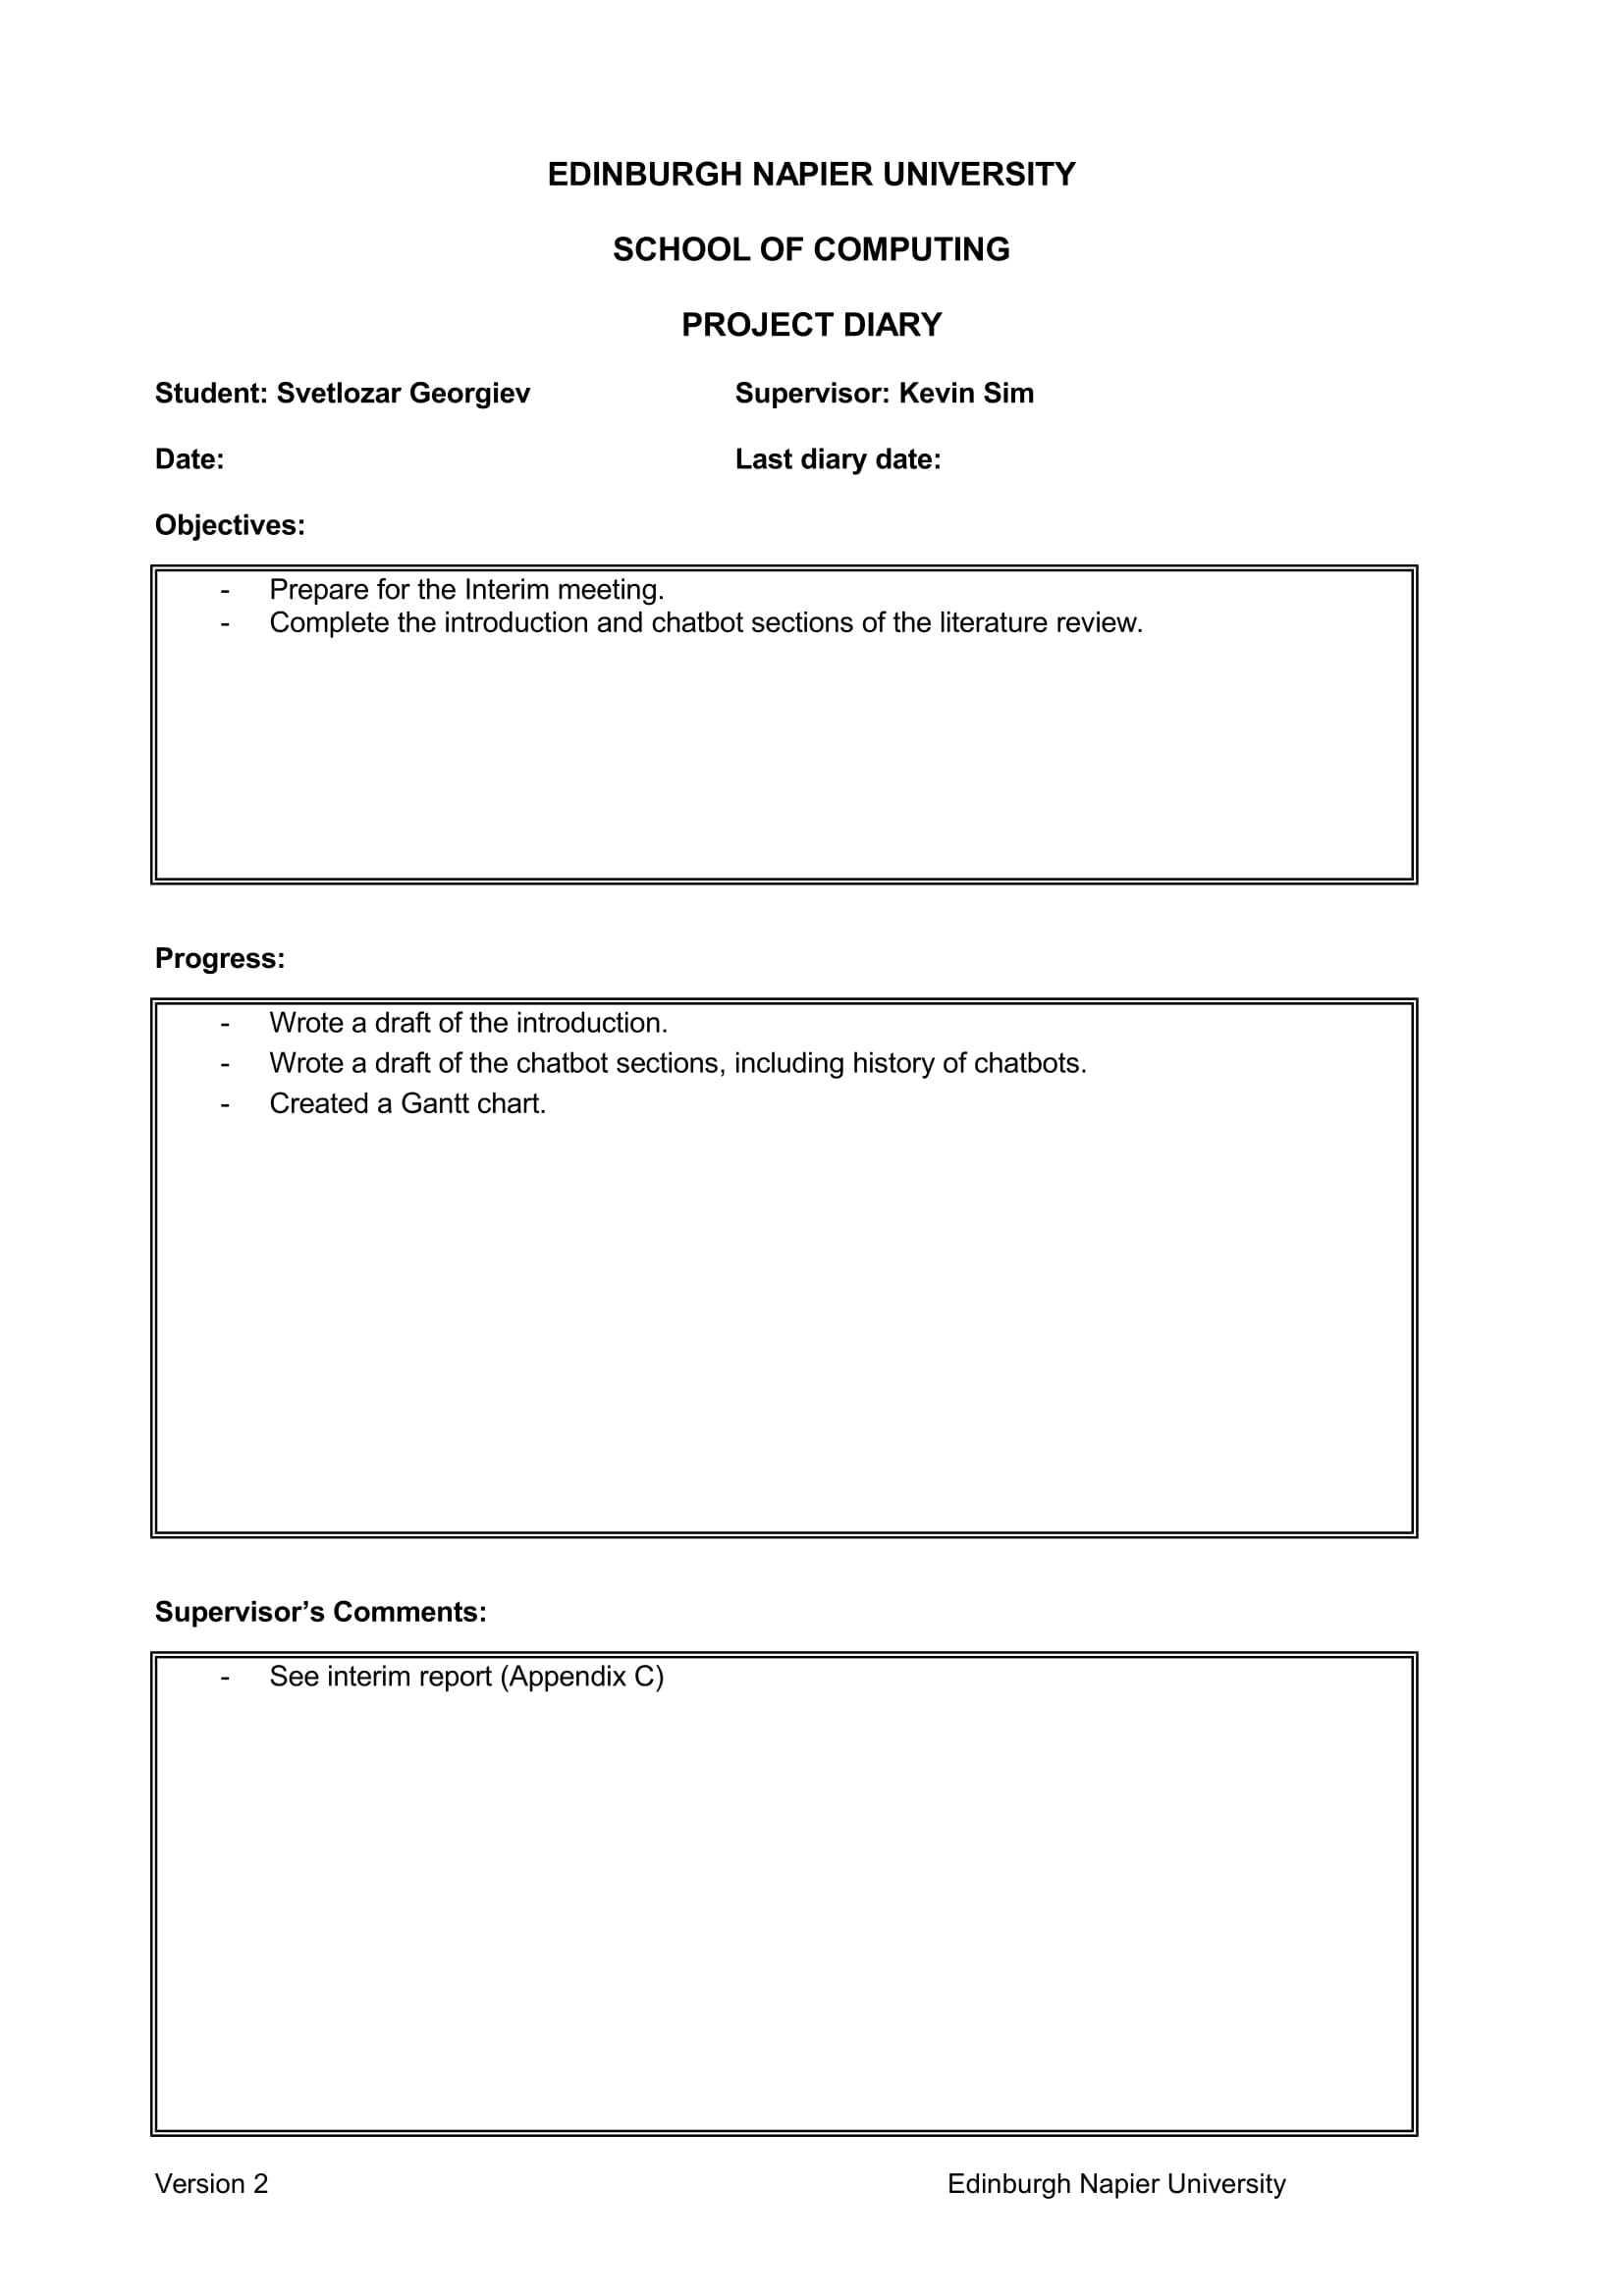
\includegraphics[width=\textwidth,height=\textheight,keepaspectratio]{week9.jpg}
% second semester
% ...
\newpage
\section{Second Formal Review Output}
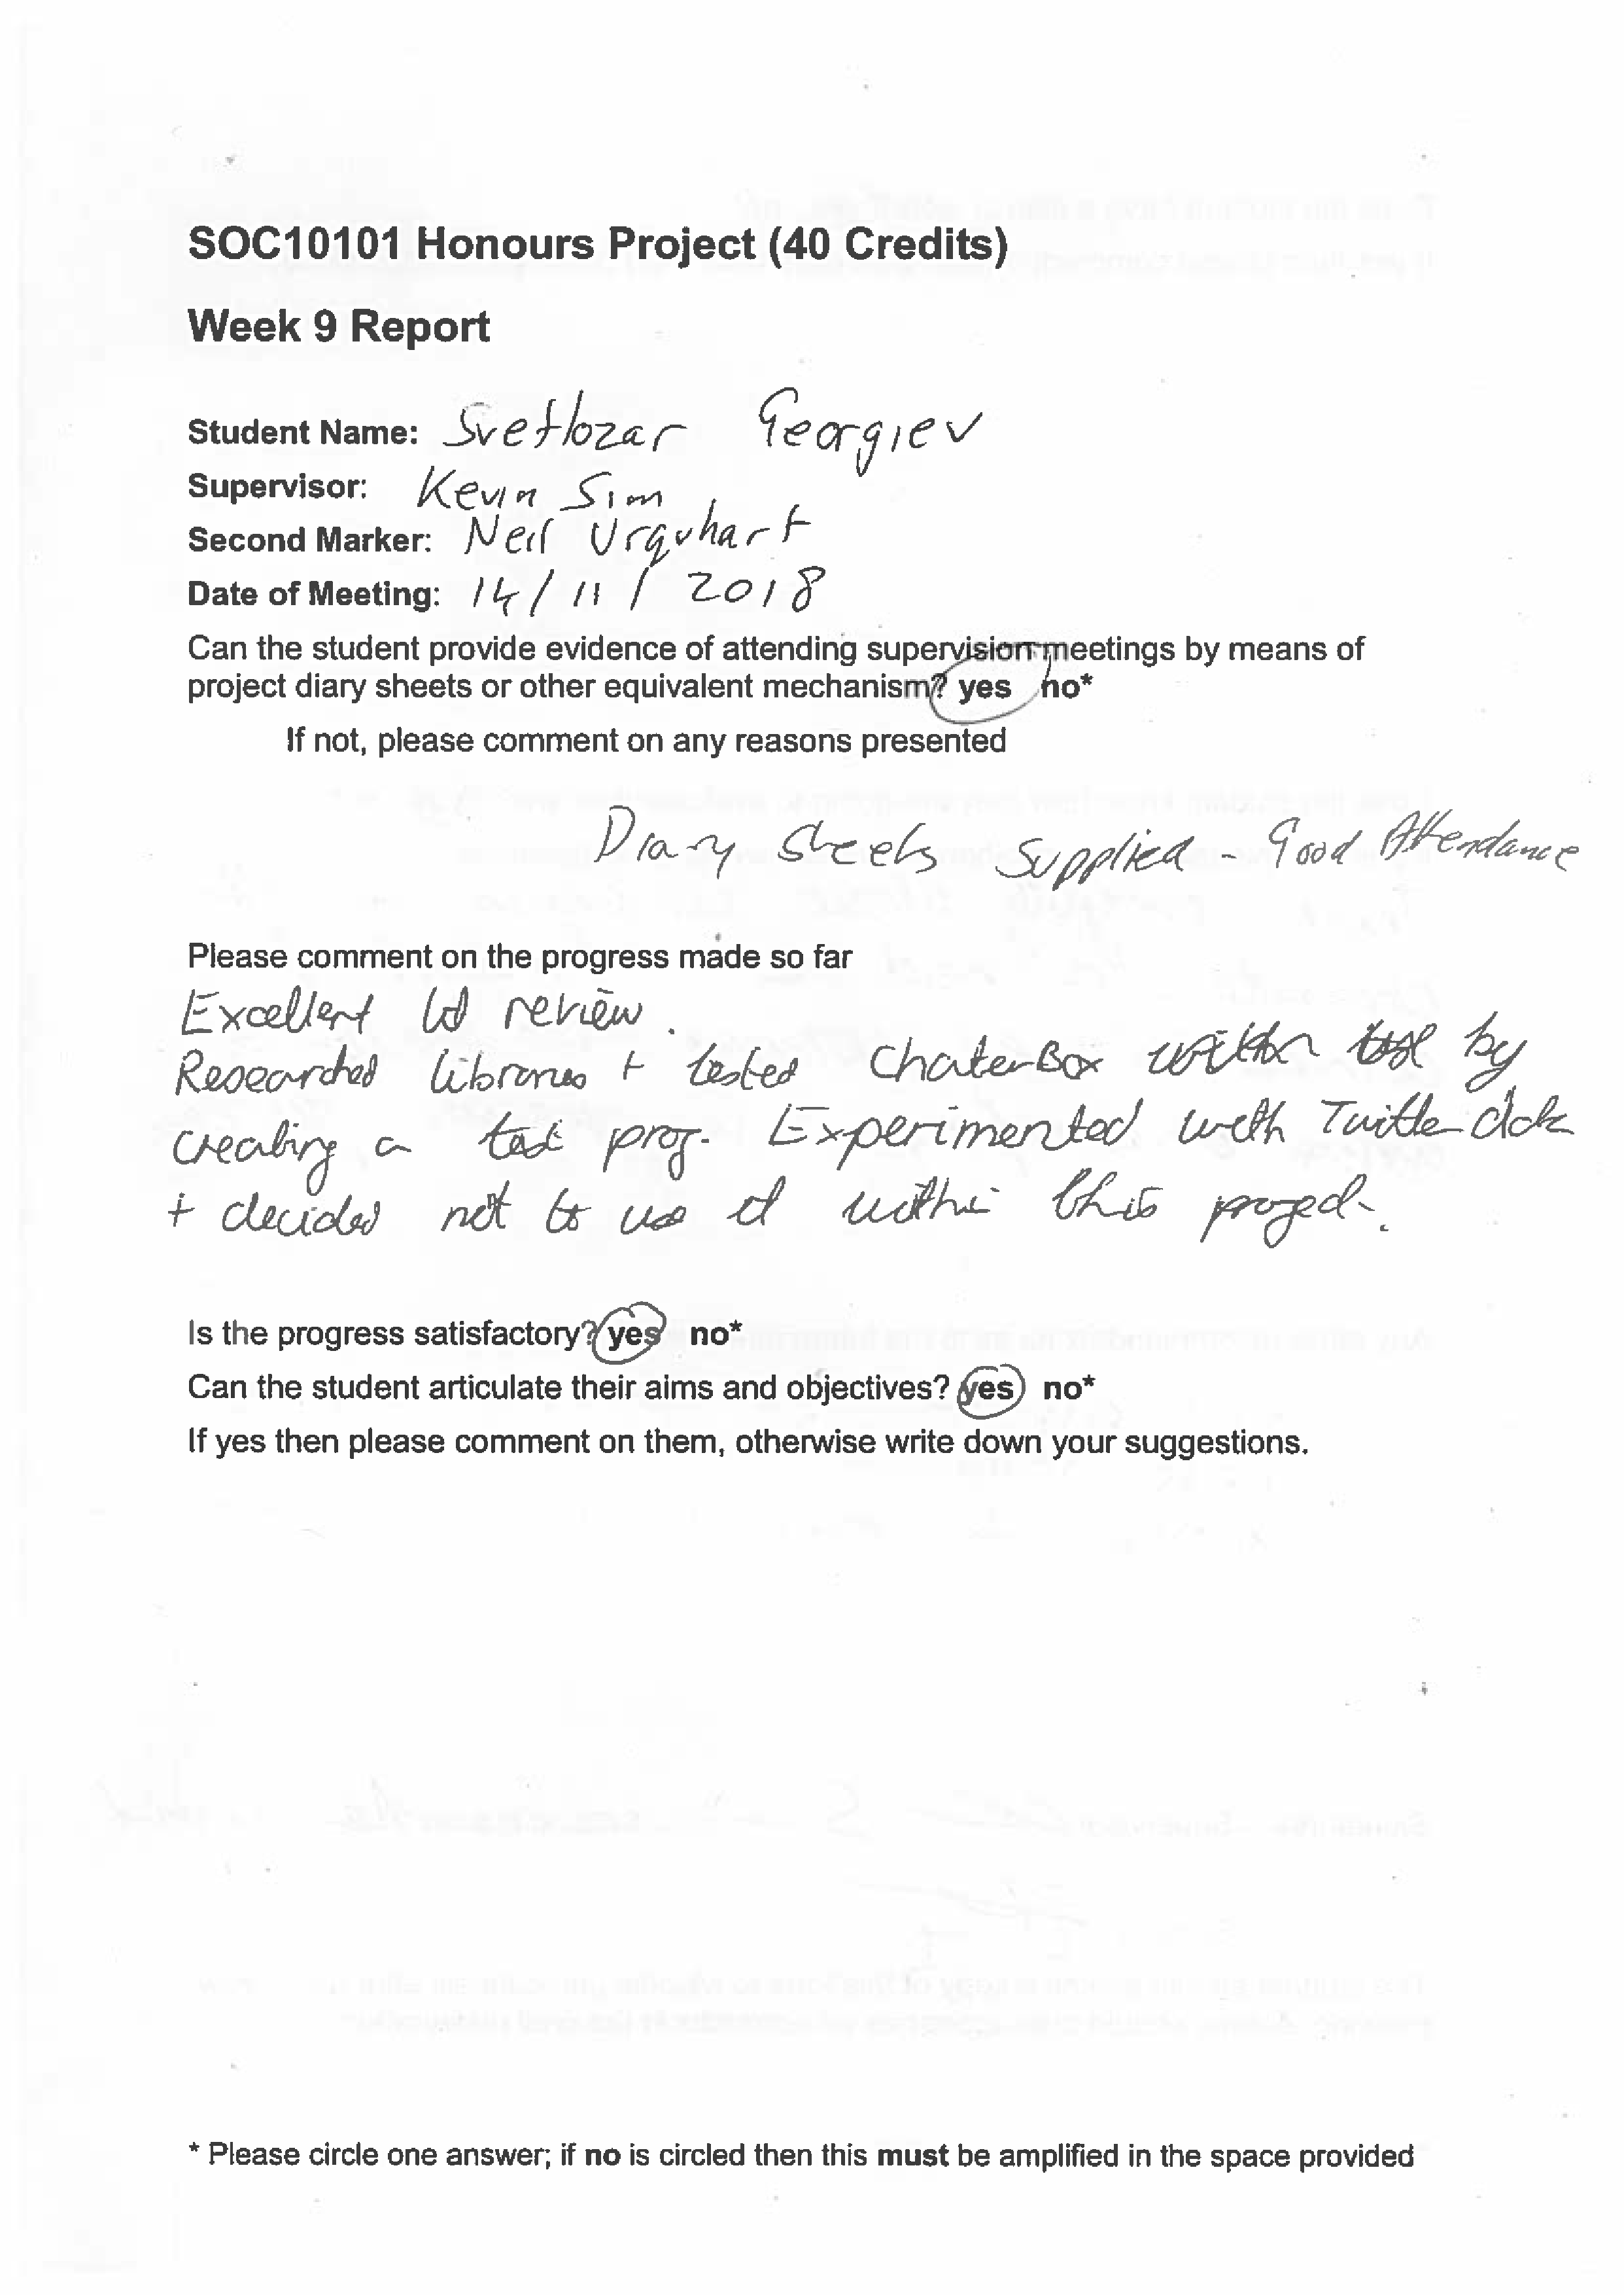
\includegraphics[width=\textwidth,height=\textheight,keepaspectratio]{interim-1.png}
\newpage
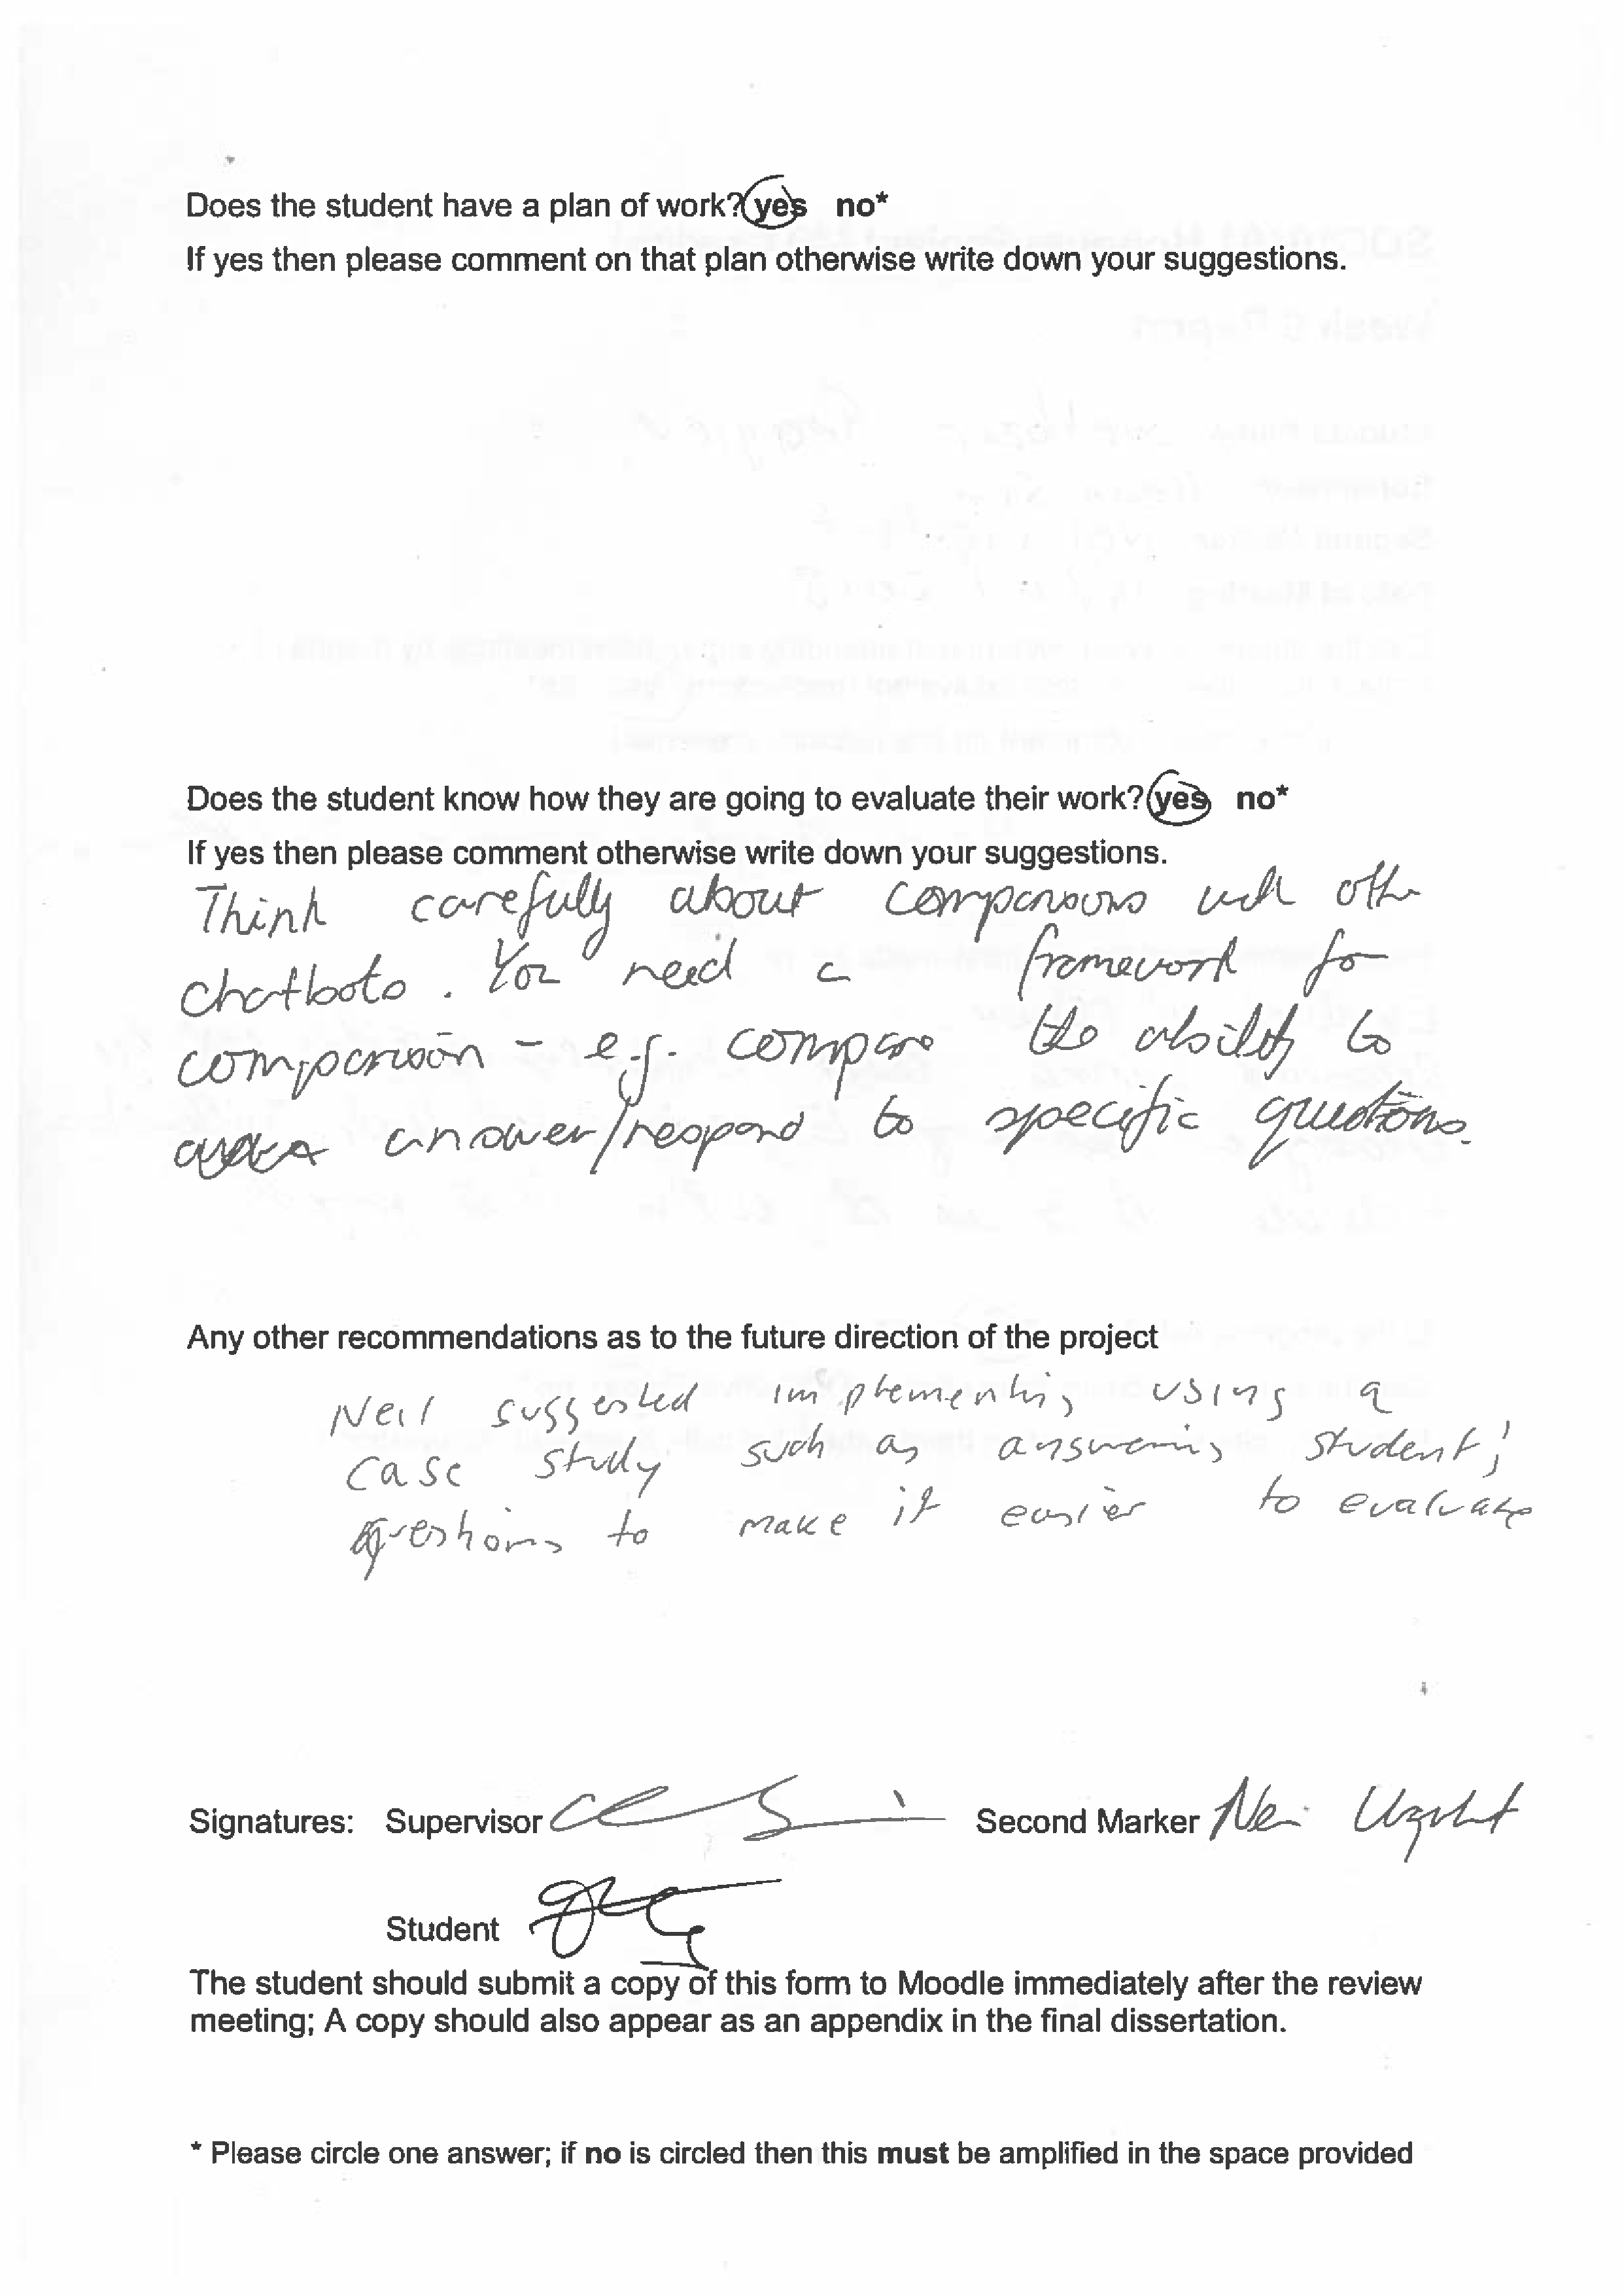
\includegraphics[width=\textwidth,height=\textheight,keepaspectratio]{interim-2.png}

\end{appendices}

\end{document}
